\section{Mesh / xy}
\clearpage\subsection*{Mean request latency}
\begin{center}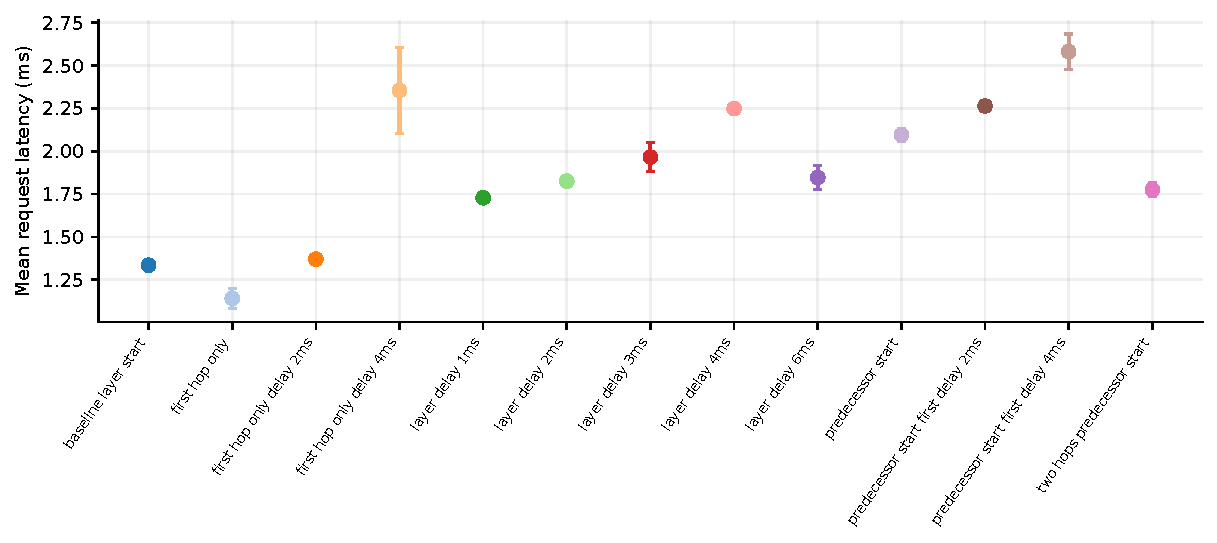
\includegraphics[width=.94\linewidth,height=.31\textheight,keepaspectratio]{figures/variants/mesh_xy_request_latency_mean_ms.pdf}\captionof{figure}{Thirteen Dynamic launch variants, M=4 and C=3; zero-delay structural rules and delay sensitivities are distinguished in the definitions.}\end{center}
\begin{center}{\scriptsize\setlength{\tabcolsep}{3pt}
\begin{tabular}{lrr}
\toprule
Variant & Mean $\pm$ SD & n \\
\midrule
baseline-layer-start & $1.335\pm0.020$ & 2 \\
first-hop-only & $1.141\pm0.058$ & 2 \\
first-hop-only-delay-2ms & $1.371\pm0.004$ & 2 \\
first-hop-only-delay-4ms & $2.354\pm0.252$ & 2 \\
layer-delay-1ms & $1.728\pm0.001$ & 2 \\
layer-delay-2ms & $1.825\pm0.005$ & 2 \\
layer-delay-3ms & $1.966\pm0.086$ & 2 \\
layer-delay-4ms & $2.248\pm0.025$ & 2 \\
layer-delay-6ms & $1.847\pm0.071$ & 2 \\
predecessor-start & $2.096\pm0.039$ & 2 \\
predecessor-start-first-delay-2ms & $2.264\pm0.030$ & 2 \\
predecessor-start-first-delay-4ms & $2.581\pm0.103$ & 2 \\
two-hops-predecessor-start & $1.775\pm0.041$ & 2 \\
\bottomrule\end{tabular}}
\captionof{table}{All thirteen variants; n counts byte-distinct trace/physics runs, not conceptual aliases.}
{\footnotesize\href{https://github.com/sanjeevkrishnaa/Compiler-Driven-ACE/blob/codex/ace-scheduler-correctness/docs/latex/qft96_final/data/variants_mesh_xy_request_latency_mean_ms.csv}{Exact CSV values and sample counts}}
\end{center}
\clearpage\subsection*{Median request latency}
\begin{center}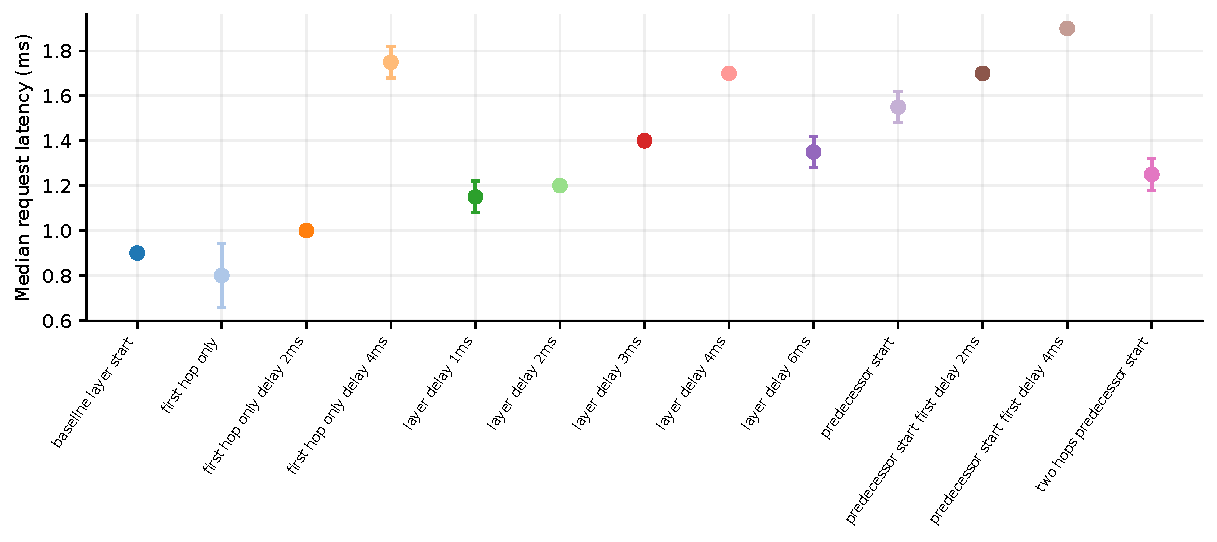
\includegraphics[width=.94\linewidth,height=.31\textheight,keepaspectratio]{figures/variants/mesh_xy_request_latency_median_ms.pdf}\captionof{figure}{Thirteen Dynamic launch variants, M=4 and C=3; zero-delay structural rules and delay sensitivities are distinguished in the definitions.}\end{center}
\begin{center}{\scriptsize\setlength{\tabcolsep}{3pt}
\begin{tabular}{lrr}
\toprule
Variant & Mean $\pm$ SD & n \\
\midrule
baseline-layer-start & $0.9000\pm0.0000$ & 2 \\
first-hop-only & $0.8000\pm0.1414$ & 2 \\
first-hop-only-delay-2ms & $1.000\pm0.000$ & 2 \\
first-hop-only-delay-4ms & $1.750\pm0.071$ & 2 \\
layer-delay-1ms & $1.150\pm0.071$ & 2 \\
layer-delay-2ms & $1.200\pm0.000$ & 2 \\
layer-delay-3ms & $1.400\pm0.000$ & 2 \\
layer-delay-4ms & $1.700\pm0.000$ & 2 \\
layer-delay-6ms & $1.350\pm0.071$ & 2 \\
predecessor-start & $1.550\pm0.071$ & 2 \\
predecessor-start-first-delay-2ms & $1.700\pm0.000$ & 2 \\
predecessor-start-first-delay-4ms & $1.900\pm0.000$ & 2 \\
two-hops-predecessor-start & $1.250\pm0.071$ & 2 \\
\bottomrule\end{tabular}}
\captionof{table}{All thirteen variants; n counts byte-distinct trace/physics runs, not conceptual aliases.}
{\footnotesize\href{https://github.com/sanjeevkrishnaa/Compiler-Driven-ACE/blob/codex/ace-scheduler-correctness/docs/latex/qft96_final/data/variants_mesh_xy_request_latency_median_ms.csv}{Exact CSV values and sample counts}}
\end{center}
\clearpage\subsection*{p95 request latency}
\begin{center}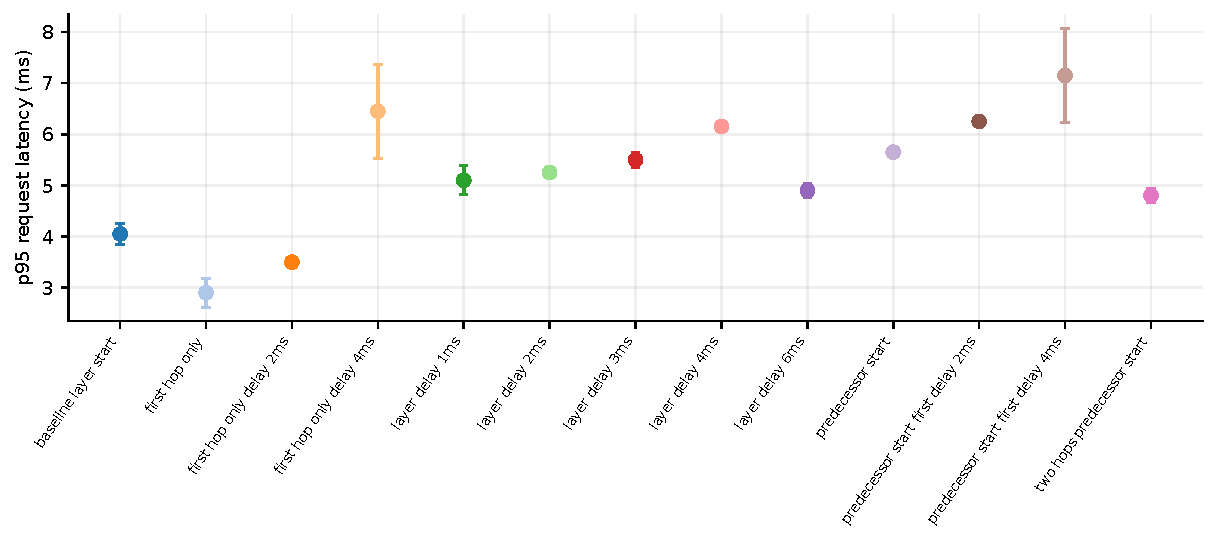
\includegraphics[width=.94\linewidth,height=.31\textheight,keepaspectratio]{figures/variants/mesh_xy_request_latency_p95_ms.pdf}\captionof{figure}{Thirteen Dynamic launch variants, M=4 and C=3; zero-delay structural rules and delay sensitivities are distinguished in the definitions.}\end{center}
\begin{center}{\scriptsize\setlength{\tabcolsep}{3pt}
\begin{tabular}{lrr}
\toprule
Variant & Mean $\pm$ SD & n \\
\midrule
baseline-layer-start & $4.050\pm0.212$ & 2 \\
first-hop-only & $2.900\pm0.283$ & 2 \\
first-hop-only-delay-2ms & $3.500\pm0.000$ & 2 \\
first-hop-only-delay-4ms & $6.450\pm0.919$ & 2 \\
layer-delay-1ms & $5.100\pm0.283$ & 2 \\
layer-delay-2ms & $5.250\pm0.071$ & 2 \\
layer-delay-3ms & $5.500\pm0.141$ & 2 \\
layer-delay-4ms & $6.150\pm0.071$ & 2 \\
layer-delay-6ms & $4.900\pm0.141$ & 2 \\
predecessor-start & $5.650\pm0.071$ & 2 \\
predecessor-start-first-delay-2ms & $6.250\pm0.071$ & 2 \\
predecessor-start-first-delay-4ms & $7.150\pm0.919$ & 2 \\
two-hops-predecessor-start & $4.800\pm0.141$ & 2 \\
\bottomrule\end{tabular}}
\captionof{table}{All thirteen variants; n counts byte-distinct trace/physics runs, not conceptual aliases.}
{\footnotesize\href{https://github.com/sanjeevkrishnaa/Compiler-Driven-ACE/blob/codex/ace-scheduler-correctness/docs/latex/qft96_final/data/variants_mesh_xy_request_latency_p95_ms.csv}{Exact CSV values and sample counts}}
\end{center}
\clearpage\subsection*{Maximum request latency}
\begin{center}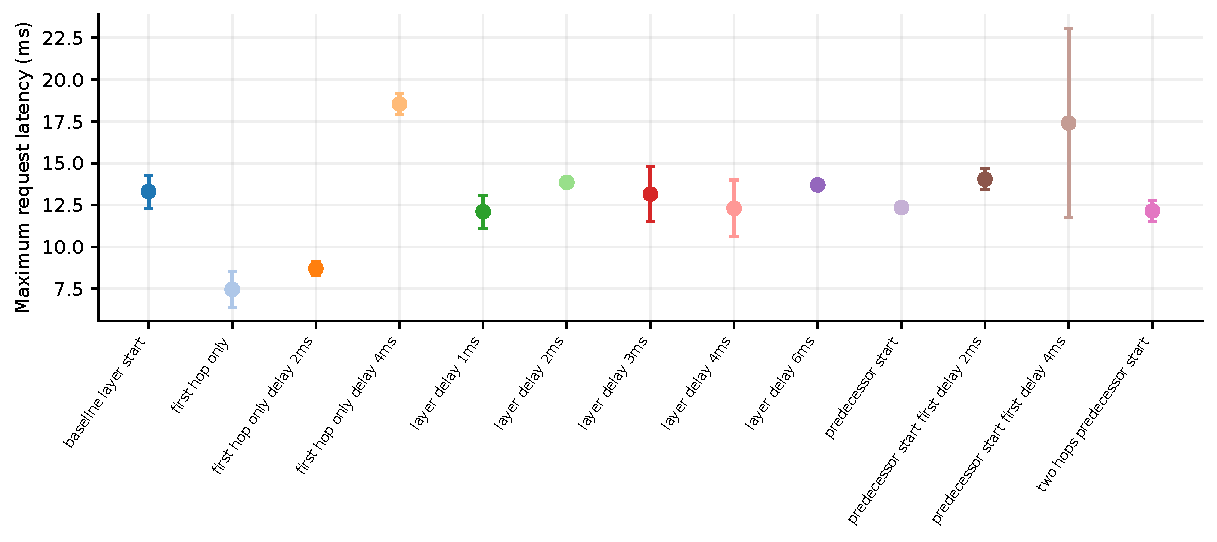
\includegraphics[width=.94\linewidth,height=.31\textheight,keepaspectratio]{figures/variants/mesh_xy_request_latency_max_ms.pdf}\captionof{figure}{Thirteen Dynamic launch variants, M=4 and C=3; zero-delay structural rules and delay sensitivities are distinguished in the definitions.}\end{center}
\begin{center}{\scriptsize\setlength{\tabcolsep}{3pt}
\begin{tabular}{lrr}
\toprule
Variant & Mean $\pm$ SD & n \\
\midrule
baseline-layer-start & $13.300\pm0.990$ & 2 \\
first-hop-only & $7.450\pm1.061$ & 2 \\
first-hop-only-delay-2ms & $8.700\pm0.424$ & 2 \\
first-hop-only-delay-4ms & $18.550\pm0.636$ & 2 \\
layer-delay-1ms & $12.100\pm0.990$ & 2 \\
layer-delay-2ms & $13.850\pm0.071$ & 2 \\
layer-delay-3ms & $13.150\pm1.626$ & 2 \\
layer-delay-4ms & $12.300\pm1.697$ & 2 \\
layer-delay-6ms & $13.700\pm0.141$ & 2 \\
predecessor-start & $12.350\pm0.071$ & 2 \\
predecessor-start-first-delay-2ms & $14.050\pm0.636$ & 2 \\
predecessor-start-first-delay-4ms & $17.400\pm5.657$ & 2 \\
two-hops-predecessor-start & $12.150\pm0.636$ & 2 \\
\bottomrule\end{tabular}}
\captionof{table}{All thirteen variants; n counts byte-distinct trace/physics runs, not conceptual aliases.}
{\footnotesize\href{https://github.com/sanjeevkrishnaa/Compiler-Driven-ACE/blob/codex/ace-scheduler-correctness/docs/latex/qft96_final/data/variants_mesh_xy_request_latency_max_ms.csv}{Exact CSV values and sample counts}}
\end{center}
\clearpage\subsection*{Communication makespan}
\begin{center}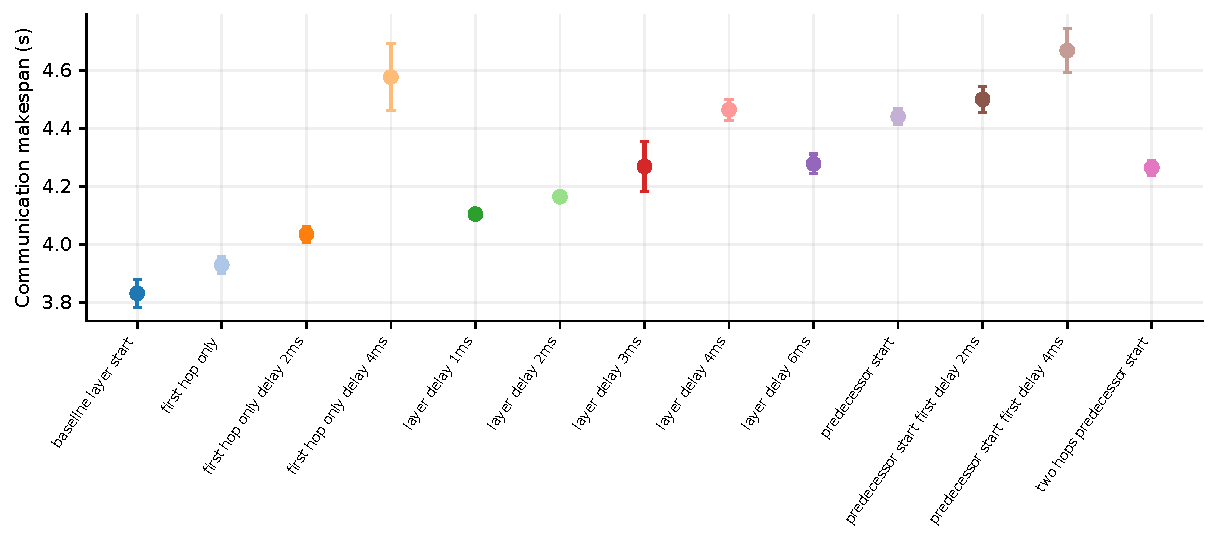
\includegraphics[width=.94\linewidth,height=.31\textheight,keepaspectratio]{figures/variants/mesh_xy_end_to_end_latency_ms.pdf}\captionof{figure}{Thirteen Dynamic launch variants, M=4 and C=3; zero-delay structural rules and delay sensitivities are distinguished in the definitions.}\end{center}
\begin{center}{\scriptsize\setlength{\tabcolsep}{3pt}
\begin{tabular}{lrr}
\toprule
Variant & Mean $\pm$ SD & n \\
\midrule
baseline-layer-start & $3.830\pm0.048$ & 2 \\
first-hop-only & $3.928\pm0.029$ & 2 \\
first-hop-only-delay-2ms & $4.034\pm0.027$ & 2 \\
first-hop-only-delay-4ms & $4.576\pm0.116$ & 2 \\
layer-delay-1ms & $4.104\pm0.006$ & 2 \\
layer-delay-2ms & $4.164\pm0.003$ & 2 \\
layer-delay-3ms & $4.268\pm0.085$ & 2 \\
layer-delay-4ms & $4.463\pm0.036$ & 2 \\
layer-delay-6ms & $4.277\pm0.034$ & 2 \\
predecessor-start & $4.441\pm0.028$ & 2 \\
predecessor-start-first-delay-2ms & $4.499\pm0.045$ & 2 \\
predecessor-start-first-delay-4ms & $4.668\pm0.076$ & 2 \\
two-hops-predecessor-start & $4.264\pm0.026$ & 2 \\
\bottomrule\end{tabular}}
\captionof{table}{All thirteen variants; n counts byte-distinct trace/physics runs, not conceptual aliases.}
{\footnotesize\href{https://github.com/sanjeevkrishnaa/Compiler-Driven-ACE/blob/codex/ace-scheduler-correctness/docs/latex/qft96_final/data/variants_mesh_xy_end_to_end_latency_ms.csv}{Exact CSV values and sample counts}}
\end{center}
\clearpage\subsection*{Mean admission wait}
\begin{center}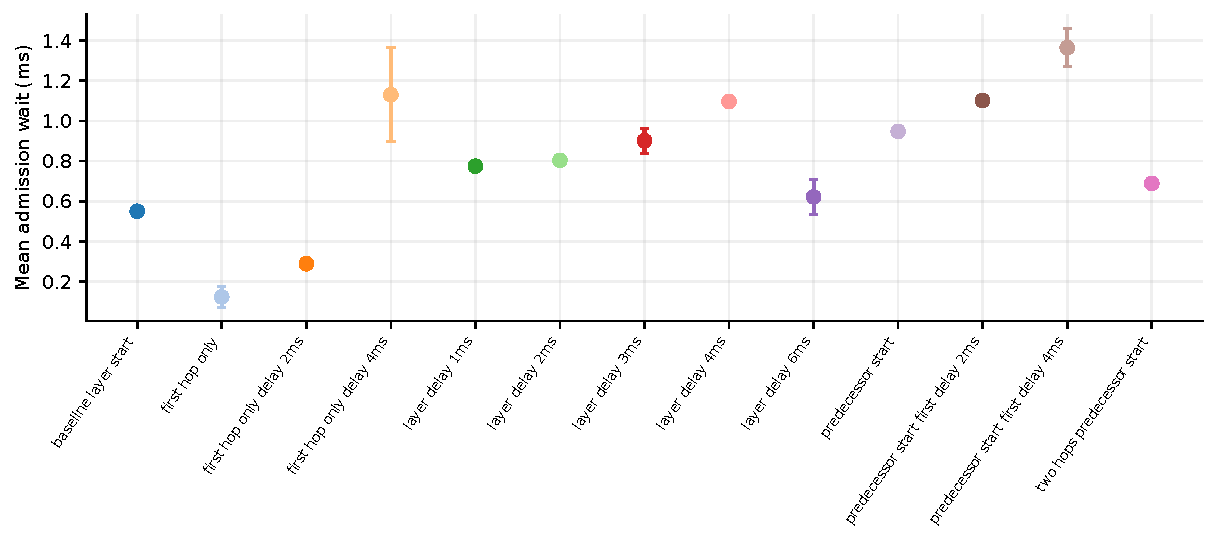
\includegraphics[width=.94\linewidth,height=.31\textheight,keepaspectratio]{figures/variants/mesh_xy_average_admission_wait_ms.pdf}\captionof{figure}{Thirteen Dynamic launch variants, M=4 and C=3; zero-delay structural rules and delay sensitivities are distinguished in the definitions.}\end{center}
\begin{center}{\scriptsize\setlength{\tabcolsep}{3pt}
\begin{tabular}{lrr}
\toprule
Variant & Mean $\pm$ SD & n \\
\midrule
baseline-layer-start & $0.5507\pm0.0249$ & 2 \\
first-hop-only & $0.1248\pm0.0514$ & 2 \\
first-hop-only-delay-2ms & $0.2897\pm0.0040$ & 2 \\
first-hop-only-delay-4ms & $1.130\pm0.234$ & 2 \\
layer-delay-1ms & $0.7748\pm0.0117$ & 2 \\
layer-delay-2ms & $0.8042\pm0.0082$ & 2 \\
layer-delay-3ms & $0.9014\pm0.0624$ & 2 \\
layer-delay-4ms & $1.097\pm0.015$ & 2 \\
layer-delay-6ms & $0.6224\pm0.0862$ & 2 \\
predecessor-start & $0.9482\pm0.0228$ & 2 \\
predecessor-start-first-delay-2ms & $1.102\pm0.019$ & 2 \\
predecessor-start-first-delay-4ms & $1.364\pm0.096$ & 2 \\
two-hops-predecessor-start & $0.6891\pm0.0128$ & 2 \\
\bottomrule\end{tabular}}
\captionof{table}{All thirteen variants; n counts byte-distinct trace/physics runs, not conceptual aliases.}
{\footnotesize\href{https://github.com/sanjeevkrishnaa/Compiler-Driven-ACE/blob/codex/ace-scheduler-correctness/docs/latex/qft96_final/data/variants_mesh_xy_average_admission_wait_ms.csv}{Exact CSV values and sample counts}}
\end{center}
\clearpage\subsection*{Delivered EPR fidelity}
\begin{center}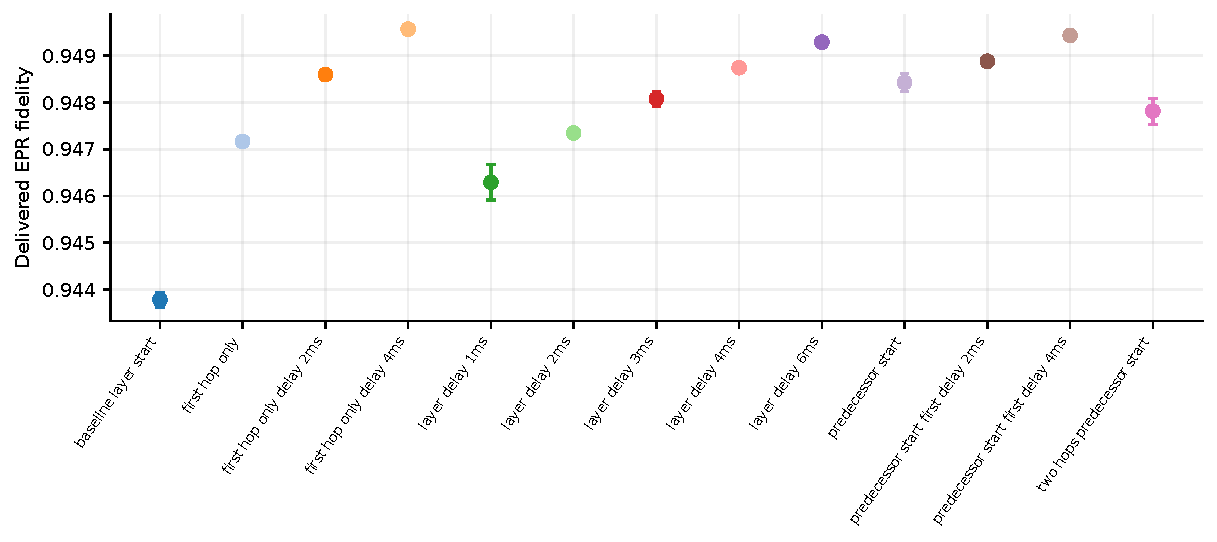
\includegraphics[width=.94\linewidth,height=.31\textheight,keepaspectratio]{figures/variants/mesh_xy_average_delivered_epr_fidelity.pdf}\captionof{figure}{Thirteen Dynamic launch variants, M=4 and C=3; zero-delay structural rules and delay sensitivities are distinguished in the definitions.}\end{center}
\begin{center}{\scriptsize\setlength{\tabcolsep}{3pt}
\begin{tabular}{lrr}
\toprule
Variant & Mean $\pm$ SD & n \\
\midrule
baseline-layer-start & $0.9438\pm0.0002$ & 2 \\
first-hop-only & $0.9472\pm0.0000$ & 2 \\
first-hop-only-delay-2ms & $0.9486\pm0.0001$ & 2 \\
first-hop-only-delay-4ms & $0.9496\pm0.0000$ & 2 \\
layer-delay-1ms & $0.9463\pm0.0004$ & 2 \\
layer-delay-2ms & $0.9473\pm0.0000$ & 2 \\
layer-delay-3ms & $0.9481\pm0.0002$ & 2 \\
layer-delay-4ms & $0.9487\pm0.0000$ & 2 \\
layer-delay-6ms & $0.9493\pm0.0000$ & 2 \\
predecessor-start & $0.9484\pm0.0002$ & 2 \\
predecessor-start-first-delay-2ms & $0.9489\pm0.0001$ & 2 \\
predecessor-start-first-delay-4ms & $0.9494\pm0.0000$ & 2 \\
two-hops-predecessor-start & $0.9478\pm0.0003$ & 2 \\
\bottomrule\end{tabular}}
\captionof{table}{All thirteen variants; n counts byte-distinct trace/physics runs, not conceptual aliases.}
{\footnotesize\href{https://github.com/sanjeevkrishnaa/Compiler-Driven-ACE/blob/codex/ace-scheduler-correctness/docs/latex/qft96_final/data/variants_mesh_xy_average_delivered_epr_fidelity.csv}{Exact CSV values and sample counts}}
\end{center}
\clearpage\subsection*{Compiler readiness fraction}
\begin{center}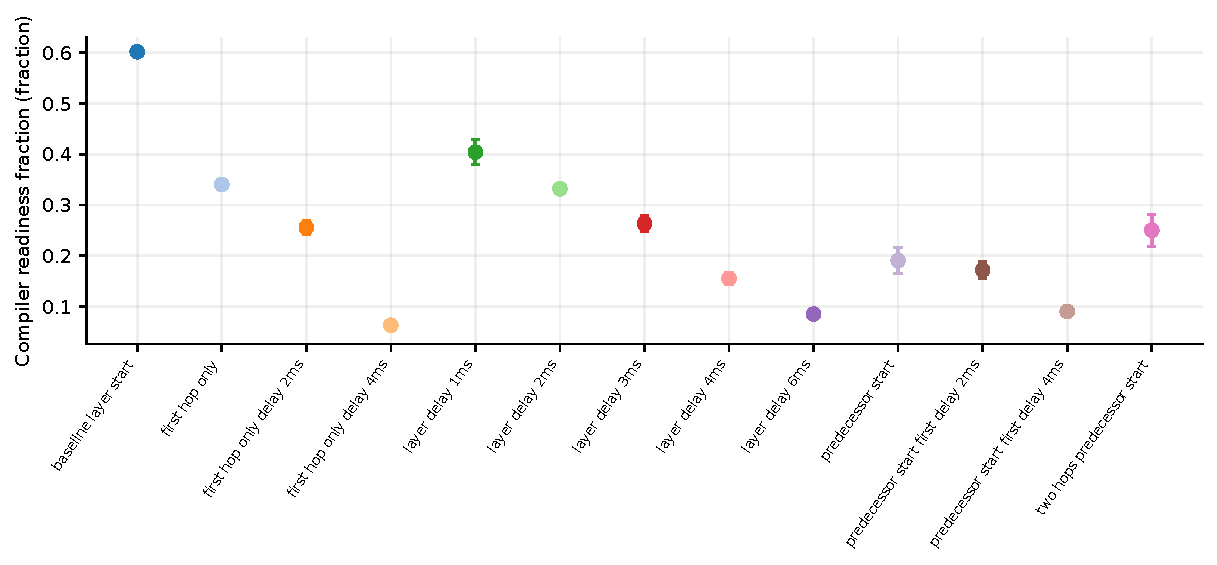
\includegraphics[width=.94\linewidth,height=.31\textheight,keepaspectratio]{figures/variants/mesh_xy_pregenerated_success_rate.pdf}\captionof{figure}{Thirteen Dynamic launch variants, M=4 and C=3; zero-delay structural rules and delay sensitivities are distinguished in the definitions.}\end{center}
\begin{center}{\scriptsize\setlength{\tabcolsep}{3pt}
\begin{tabular}{lrr}
\toprule
Variant & Mean $\pm$ SD & n \\
\midrule
baseline-layer-start & $0.6017\pm0.0007$ & 2 \\
first-hop-only & $0.3403\pm0.0044$ & 2 \\
first-hop-only-delay-2ms & $0.2557\pm0.0128$ & 2 \\
first-hop-only-delay-4ms & $0.0632\pm0.0099$ & 2 \\
layer-delay-1ms & $0.4040\pm0.0244$ & 2 \\
layer-delay-2ms & $0.3318\pm0.0015$ & 2 \\
layer-delay-3ms & $0.2637\pm0.0157$ & 2 \\
layer-delay-4ms & $0.1552\pm0.0119$ & 2 \\
layer-delay-6ms & $0.0851\pm0.0018$ & 2 \\
predecessor-start & $0.1905\pm0.0254$ & 2 \\
predecessor-start-first-delay-2ms & $0.1718\pm0.0168$ & 2 \\
predecessor-start-first-delay-4ms & $0.0904\pm0.0064$ & 2 \\
two-hops-predecessor-start & $0.2504\pm0.0316$ & 2 \\
\bottomrule\end{tabular}}
\captionof{table}{All thirteen variants; n counts byte-distinct trace/physics runs, not conceptual aliases.}
{\footnotesize\href{https://github.com/sanjeevkrishnaa/Compiler-Driven-ACE/blob/codex/ace-scheduler-correctness/docs/latex/qft96_final/data/variants_mesh_xy_pregenerated_success_rate.csv}{Exact CSV values and sample counts}}
\end{center}
\clearpage\subsection*{Intended compiler-hit fraction}
\begin{center}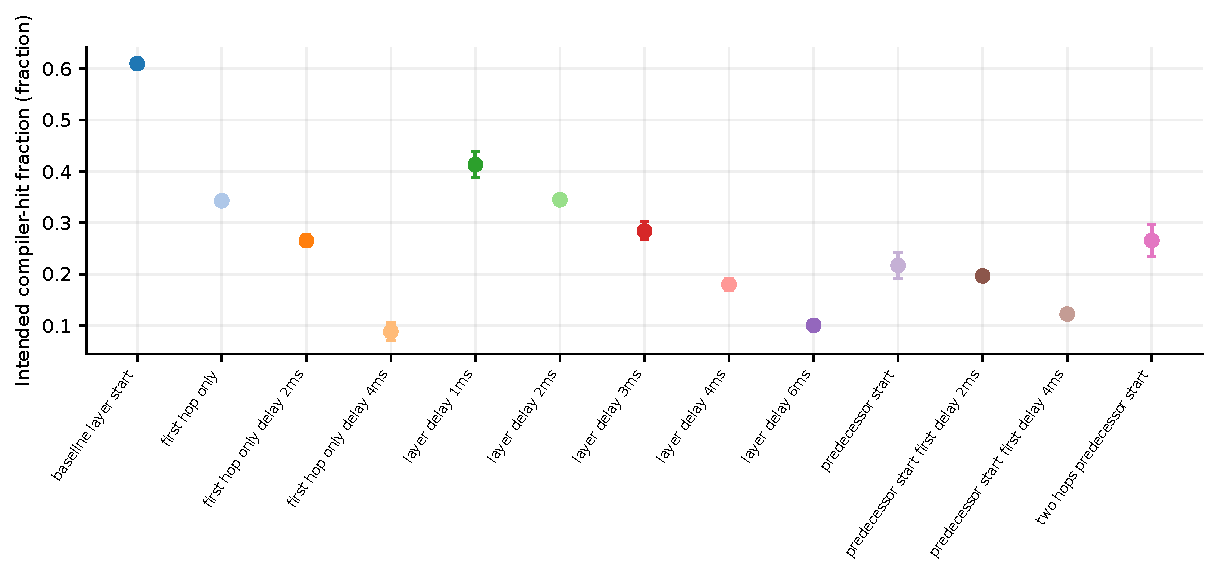
\includegraphics[width=.94\linewidth,height=.31\textheight,keepaspectratio]{figures/variants/mesh_xy_intended_request_hit_rate.pdf}\captionof{figure}{Thirteen Dynamic launch variants, M=4 and C=3; zero-delay structural rules and delay sensitivities are distinguished in the definitions.}\end{center}
\begin{center}{\scriptsize\setlength{\tabcolsep}{3pt}
\begin{tabular}{lrr}
\toprule
Variant & Mean $\pm$ SD & n \\
\midrule
baseline-layer-start & $0.6094\pm0.0044$ & 2 \\
first-hop-only & $0.3429\pm0.0033$ & 2 \\
first-hop-only-delay-2ms & $0.2655\pm0.0120$ & 2 \\
first-hop-only-delay-4ms & $0.0885\pm0.0168$ & 2 \\
layer-delay-1ms & $0.4129\pm0.0250$ & 2 \\
layer-delay-2ms & $0.3448\pm0.0009$ & 2 \\
layer-delay-3ms & $0.2843\pm0.0175$ & 2 \\
layer-delay-4ms & $0.1802\pm0.0115$ & 2 \\
layer-delay-6ms & $0.1007\pm0.0009$ & 2 \\
predecessor-start & $0.2171\pm0.0257$ & 2 \\
predecessor-start-first-delay-2ms & $0.1967\pm0.0104$ & 2 \\
predecessor-start-first-delay-4ms & $0.1225\pm0.0051$ & 2 \\
two-hops-predecessor-start & $0.2656\pm0.0316$ & 2 \\
\bottomrule\end{tabular}}
\captionof{table}{All thirteen variants; n counts byte-distinct trace/physics runs, not conceptual aliases.}
{\footnotesize\href{https://github.com/sanjeevkrishnaa/Compiler-Driven-ACE/blob/codex/ace-scheduler-correctness/docs/latex/qft96_final/data/variants_mesh_xy_intended_request_hit_rate.csv}{Exact CSV values and sample counts}}
\end{center}
\clearpage\subsection*{Compiler fallback fraction}
\begin{center}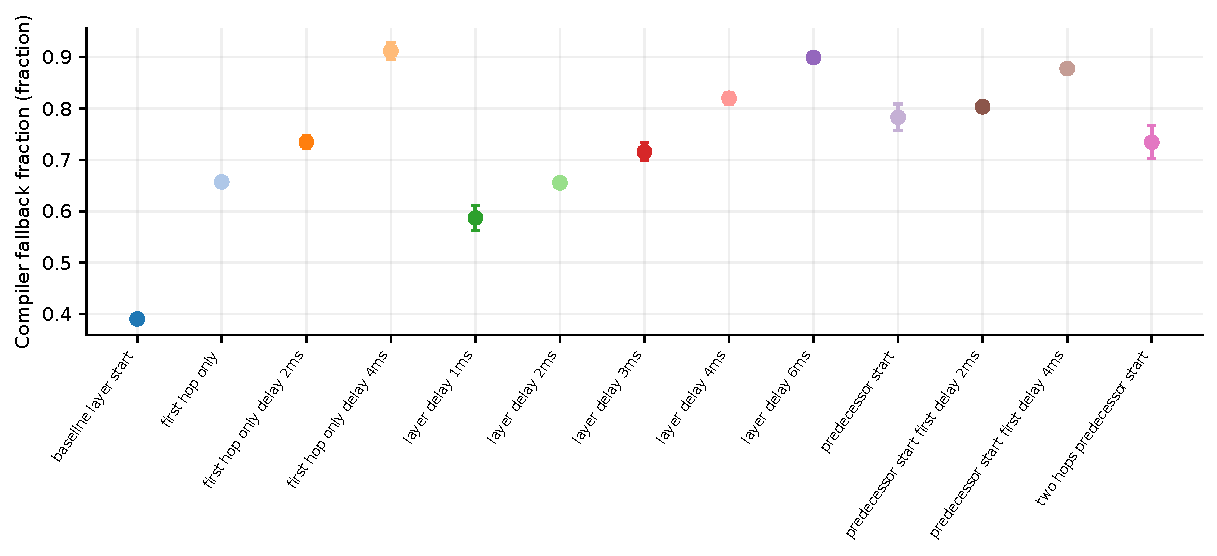
\includegraphics[width=.94\linewidth,height=.31\textheight,keepaspectratio]{figures/variants/mesh_xy_on_demand_fallback_rate.pdf}\captionof{figure}{Thirteen Dynamic launch variants, M=4 and C=3; zero-delay structural rules and delay sensitivities are distinguished in the definitions.}\end{center}
\begin{center}{\scriptsize\setlength{\tabcolsep}{3pt}
\begin{tabular}{lrr}
\toprule
Variant & Mean $\pm$ SD & n \\
\midrule
baseline-layer-start & $0.3906\pm0.0044$ & 2 \\
first-hop-only & $0.6571\pm0.0033$ & 2 \\
first-hop-only-delay-2ms & $0.7345\pm0.0120$ & 2 \\
first-hop-only-delay-4ms & $0.9115\pm0.0168$ & 2 \\
layer-delay-1ms & $0.5871\pm0.0250$ & 2 \\
layer-delay-2ms & $0.6552\pm0.0009$ & 2 \\
layer-delay-3ms & $0.7157\pm0.0175$ & 2 \\
layer-delay-4ms & $0.8198\pm0.0115$ & 2 \\
layer-delay-6ms & $0.8993\pm0.0009$ & 2 \\
predecessor-start & $0.7829\pm0.0257$ & 2 \\
predecessor-start-first-delay-2ms & $0.8033\pm0.0104$ & 2 \\
predecessor-start-first-delay-4ms & $0.8775\pm0.0051$ & 2 \\
two-hops-predecessor-start & $0.7344\pm0.0316$ & 2 \\
\bottomrule\end{tabular}}
\captionof{table}{All thirteen variants; n counts byte-distinct trace/physics runs, not conceptual aliases.}
{\footnotesize\href{https://github.com/sanjeevkrishnaa/Compiler-Driven-ACE/blob/codex/ace-scheduler-correctness/docs/latex/qft96_final/data/variants_mesh_xy_on_demand_fallback_rate.csv}{Exact CSV values and sample counts}}
\end{center}
\clearpage\subsection*{Compiler-cache waste}
\begin{center}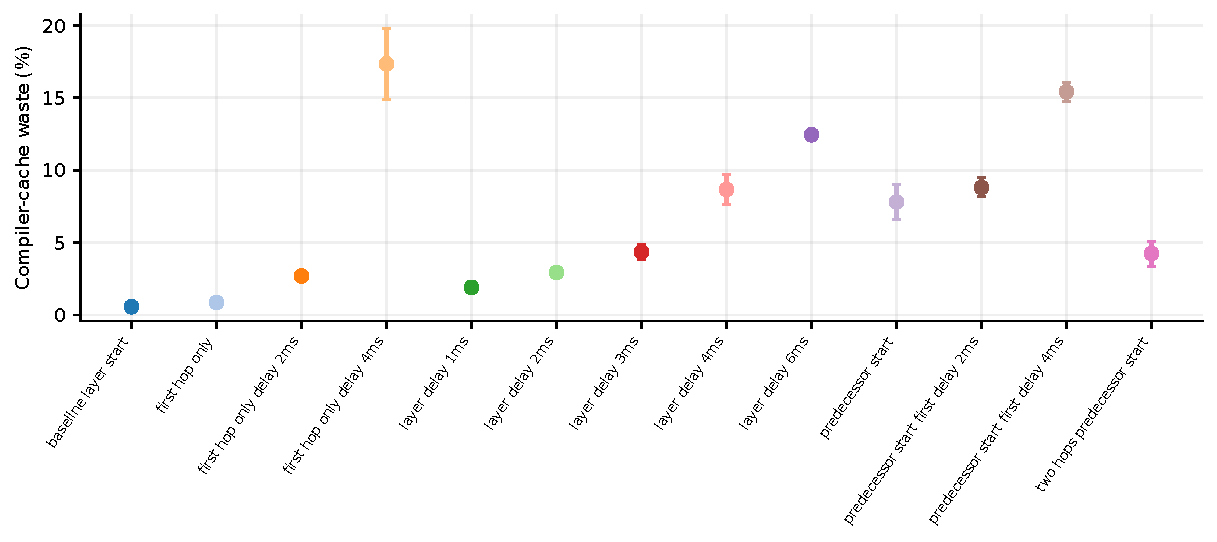
\includegraphics[width=.94\linewidth,height=.31\textheight,keepaspectratio]{figures/variants/mesh_xy_compiler_waste_percentage.pdf}\captionof{figure}{Thirteen Dynamic launch variants, M=4 and C=3; zero-delay structural rules and delay sensitivities are distinguished in the definitions.}\end{center}
\begin{center}{\scriptsize\setlength{\tabcolsep}{3pt}
\begin{tabular}{lrr}
\toprule
Variant & Mean $\pm$ SD & n \\
\midrule
baseline-layer-start & $0.5684\pm0.0337$ & 2 \\
first-hop-only & $0.8582\pm0.0604$ & 2 \\
first-hop-only-delay-2ms & $2.696\pm0.054$ & 2 \\
first-hop-only-delay-4ms & $17.346\pm2.443$ & 2 \\
layer-delay-1ms & $1.911\pm0.369$ & 2 \\
layer-delay-2ms & $2.941\pm0.142$ & 2 \\
layer-delay-3ms & $4.354\pm0.491$ & 2 \\
layer-delay-4ms & $8.660\pm1.012$ & 2 \\
layer-delay-6ms & $12.444\pm0.040$ & 2 \\
predecessor-start & $7.794\pm1.210$ & 2 \\
predecessor-start-first-delay-2ms & $8.807\pm0.656$ & 2 \\
predecessor-start-first-delay-4ms & $15.416\pm0.650$ & 2 \\
two-hops-predecessor-start & $4.235\pm0.860$ & 2 \\
\bottomrule\end{tabular}}
\captionof{table}{All thirteen variants; n counts byte-distinct trace/physics runs, not conceptual aliases.}
{\footnotesize\href{https://github.com/sanjeevkrishnaa/Compiler-Driven-ACE/blob/codex/ace-scheduler-correctness/docs/latex/qft96_final/data/variants_mesh_xy_compiler_waste_percentage.csv}{Exact CSV values and sample counts}}
\end{center}
\clearpage\subsection*{Native-protocol waste}
\begin{center}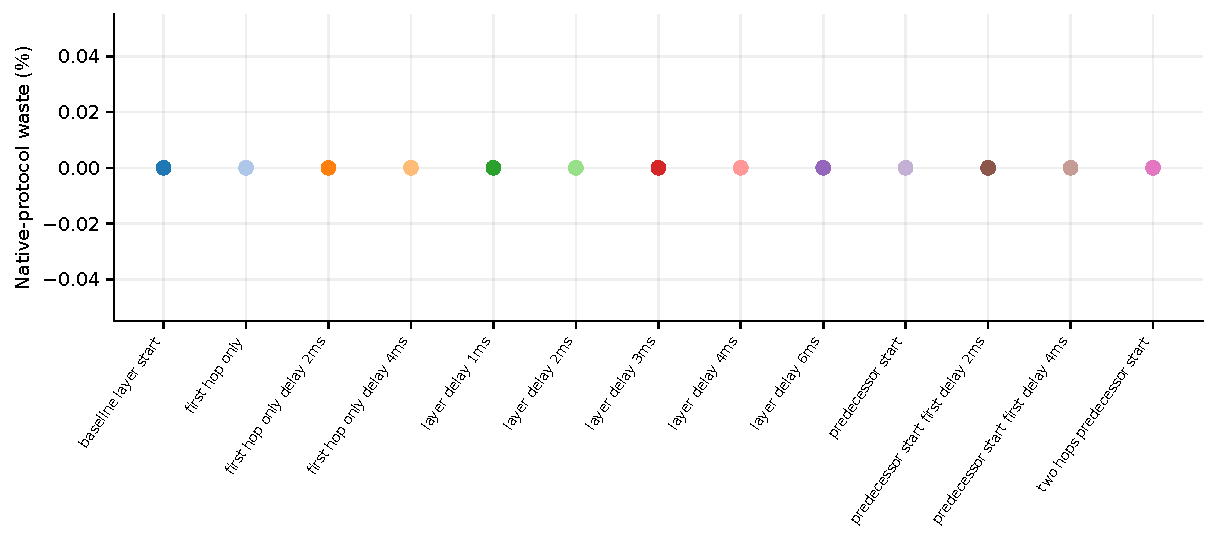
\includegraphics[width=.94\linewidth,height=.31\textheight,keepaspectratio]{figures/variants/mesh_xy_protocol_waste_percentage.pdf}\captionof{figure}{Thirteen Dynamic launch variants, M=4 and C=3; zero-delay structural rules and delay sensitivities are distinguished in the definitions.}\end{center}
\begin{center}{\scriptsize\setlength{\tabcolsep}{3pt}
\begin{tabular}{lrr}
\toprule
Variant & Mean $\pm$ SD & n \\
\midrule
baseline-layer-start & $0.0000\pm0.0000$ & 2 \\
first-hop-only & $0.0000\pm0.0000$ & 2 \\
first-hop-only-delay-2ms & $0.0000\pm0.0000$ & 2 \\
first-hop-only-delay-4ms & $0.0000\pm0.0000$ & 2 \\
layer-delay-1ms & $0.0000\pm0.0000$ & 2 \\
layer-delay-2ms & $0.0000\pm0.0000$ & 2 \\
layer-delay-3ms & $0.0000\pm0.0000$ & 2 \\
layer-delay-4ms & $0.0000\pm0.0000$ & 2 \\
layer-delay-6ms & $0.0000\pm0.0000$ & 2 \\
predecessor-start & $0.0000\pm0.0000$ & 2 \\
predecessor-start-first-delay-2ms & $0.0000\pm0.0000$ & 2 \\
predecessor-start-first-delay-4ms & $0.0000\pm0.0000$ & 2 \\
two-hops-predecessor-start & $0.0000\pm0.0000$ & 2 \\
\bottomrule\end{tabular}}
\captionof{table}{All thirteen variants; n counts byte-distinct trace/physics runs, not conceptual aliases.}
{\footnotesize\href{https://github.com/sanjeevkrishnaa/Compiler-Driven-ACE/blob/codex/ace-scheduler-correctness/docs/latex/qft96_final/data/variants_mesh_xy_protocol_waste_percentage.csv}{Exact CSV values and sample counts}}
\end{center}
\clearpage\subsection*{Compiler-pair expiry}
\begin{center}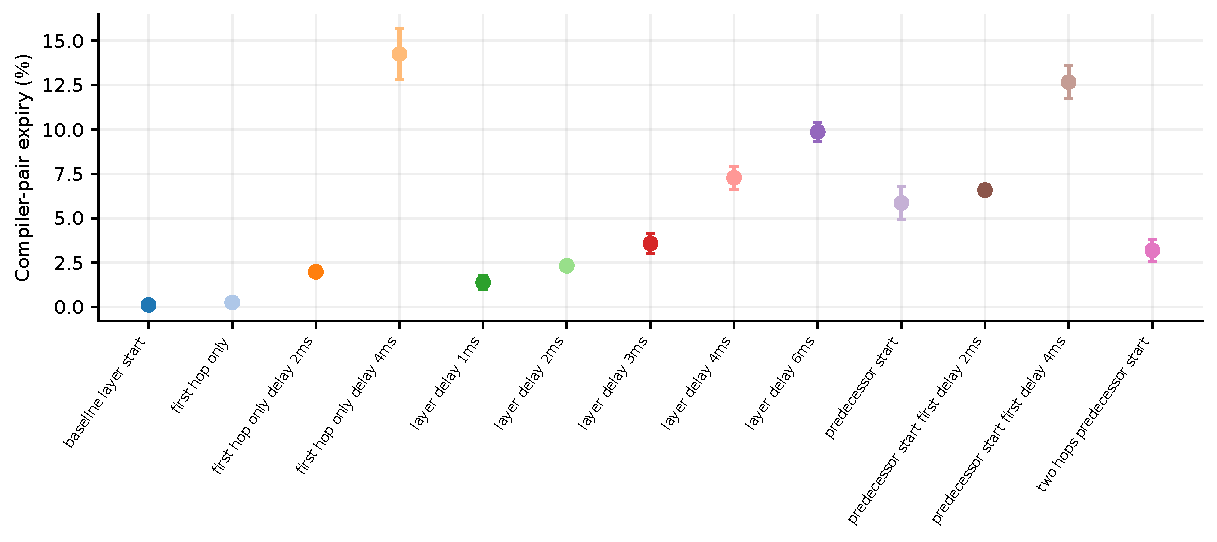
\includegraphics[width=.94\linewidth,height=.31\textheight,keepaspectratio]{figures/variants/mesh_xy_compiler_expiry_percentage.pdf}\captionof{figure}{Thirteen Dynamic launch variants, M=4 and C=3; zero-delay structural rules and delay sensitivities are distinguished in the definitions.}\end{center}
\begin{center}{\scriptsize\setlength{\tabcolsep}{3pt}
\begin{tabular}{lrr}
\toprule
Variant & Mean $\pm$ SD & n \\
\midrule
baseline-layer-start & $0.1263\pm0.0009$ & 2 \\
first-hop-only & $0.2623\pm0.2661$ & 2 \\
first-hop-only-delay-2ms & $1.988\pm0.089$ & 2 \\
first-hop-only-delay-4ms & $14.245\pm1.433$ & 2 \\
layer-delay-1ms & $1.390\pm0.382$ & 2 \\
layer-delay-2ms & $2.324\pm0.112$ & 2 \\
layer-delay-3ms & $3.575\pm0.570$ & 2 \\
layer-delay-4ms & $7.277\pm0.661$ & 2 \\
layer-delay-6ms & $9.863\pm0.540$ & 2 \\
predecessor-start & $5.860\pm0.928$ & 2 \\
predecessor-start-first-delay-2ms & $6.586\pm0.301$ & 2 \\
predecessor-start-first-delay-4ms & $12.661\pm0.934$ & 2 \\
two-hops-predecessor-start & $3.198\pm0.615$ & 2 \\
\bottomrule\end{tabular}}
\captionof{table}{All thirteen variants; n counts byte-distinct trace/physics runs, not conceptual aliases.}
{\footnotesize\href{https://github.com/sanjeevkrishnaa/Compiler-Driven-ACE/blob/codex/ace-scheduler-correctness/docs/latex/qft96_final/data/variants_mesh_xy_compiler_expiry_percentage.csv}{Exact CSV values and sample counts}}
\end{center}
\clearpage\subsection*{Used compiler-pair storage time}
\begin{center}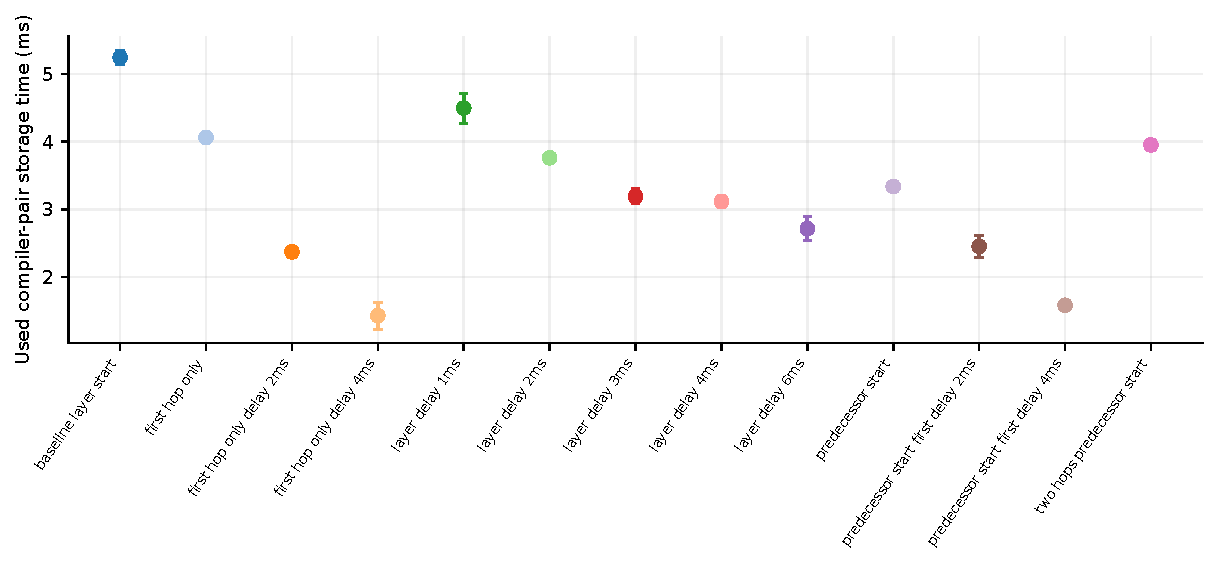
\includegraphics[width=.94\linewidth,height=.31\textheight,keepaspectratio]{figures/variants/mesh_xy_average_storage_time_ms.pdf}\captionof{figure}{Thirteen Dynamic launch variants, M=4 and C=3; zero-delay structural rules and delay sensitivities are distinguished in the definitions.}\end{center}
\begin{center}{\scriptsize\setlength{\tabcolsep}{3pt}
\begin{tabular}{lrr}
\toprule
Variant & Mean $\pm$ SD & n \\
\midrule
baseline-layer-start & $5.247\pm0.103$ & 2 \\
first-hop-only & $4.063\pm0.041$ & 2 \\
first-hop-only-delay-2ms & $2.371\pm0.078$ & 2 \\
first-hop-only-delay-4ms & $1.426\pm0.200$ & 2 \\
layer-delay-1ms & $4.497\pm0.221$ & 2 \\
layer-delay-2ms & $3.761\pm0.056$ & 2 \\
layer-delay-3ms & $3.191\pm0.110$ & 2 \\
layer-delay-4ms & $3.116\pm0.084$ & 2 \\
layer-delay-6ms & $2.714\pm0.177$ & 2 \\
predecessor-start & $3.338\pm0.078$ & 2 \\
predecessor-start-first-delay-2ms & $2.452\pm0.161$ & 2 \\
predecessor-start-first-delay-4ms & $1.580\pm0.021$ & 2 \\
two-hops-predecessor-start & $3.952\pm0.083$ & 2 \\
\bottomrule\end{tabular}}
\captionof{table}{All thirteen variants; n counts byte-distinct trace/physics runs, not conceptual aliases.}
{\footnotesize\href{https://github.com/sanjeevkrishnaa/Compiler-Driven-ACE/blob/codex/ace-scheduler-correctness/docs/latex/qft96_final/data/variants_mesh_xy_average_storage_time_ms.csv}{Exact CSV values and sample counts}}
\end{center}
\clearpage\subsection*{Delivered-hop throughput}
\begin{center}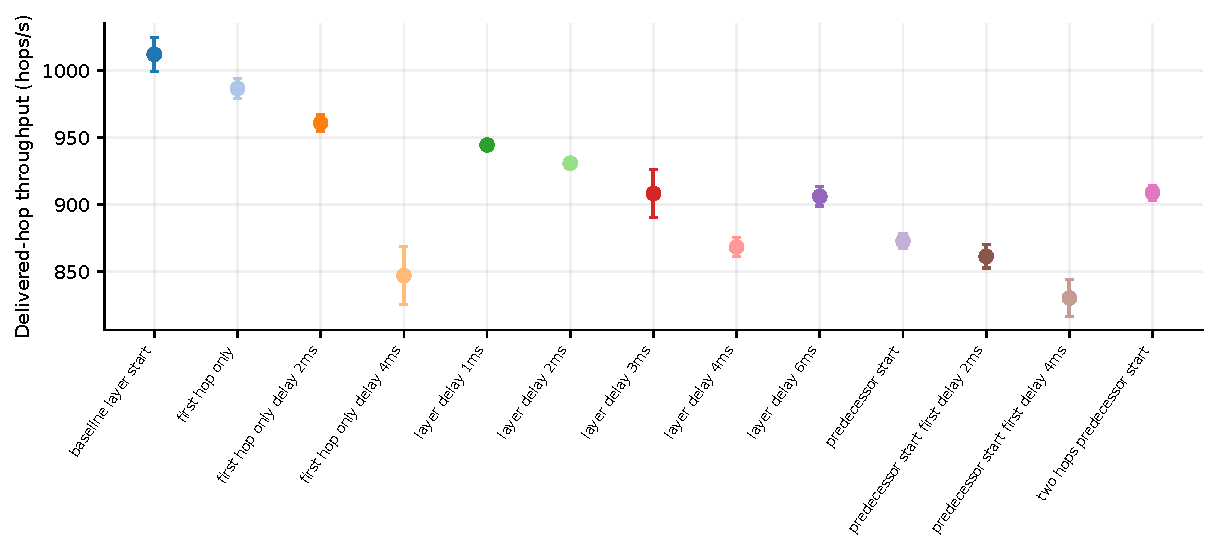
\includegraphics[width=.94\linewidth,height=.31\textheight,keepaspectratio]{figures/variants/mesh_xy_hop_throughput_s.pdf}\captionof{figure}{Thirteen Dynamic launch variants, M=4 and C=3; zero-delay structural rules and delay sensitivities are distinguished in the definitions.}\end{center}
\begin{center}{\scriptsize\setlength{\tabcolsep}{3pt}
\begin{tabular}{lrr}
\toprule
Variant & Mean $\pm$ SD & n \\
\midrule
baseline-layer-start & $1012.03\pm12.59$ & 2 \\
first-hop-only & $986.67\pm7.33$ & 2 \\
first-hop-only-delay-2ms & $960.87\pm6.54$ & 2 \\
first-hop-only-delay-4ms & $847.21\pm21.46$ & 2 \\
layer-delay-1ms & $944.48\pm1.37$ & 2 \\
layer-delay-2ms & $930.93\pm0.77$ & 2 \\
layer-delay-3ms & $908.35\pm18.06$ & 2 \\
layer-delay-4ms & $868.44\pm7.04$ & 2 \\
layer-delay-6ms & $906.18\pm7.13$ & 2 \\
predecessor-start & $872.87\pm5.55$ & 2 \\
predecessor-start-first-delay-2ms & $861.47\pm8.63$ & 2 \\
predecessor-start-first-delay-4ms & $830.45\pm13.55$ & 2 \\
two-hops-predecessor-start & $908.96\pm5.44$ & 2 \\
\bottomrule\end{tabular}}
\captionof{table}{All thirteen variants; n counts byte-distinct trace/physics runs, not conceptual aliases.}
{\footnotesize\href{https://github.com/sanjeevkrishnaa/Compiler-Driven-ACE/blob/codex/ace-scheduler-correctness/docs/latex/qft96_final/data/variants_mesh_xy_hop_throughput_s.csv}{Exact CSV values and sample counts}}
\end{center}
\clearpage\subsection*{Completion fraction}
\begin{center}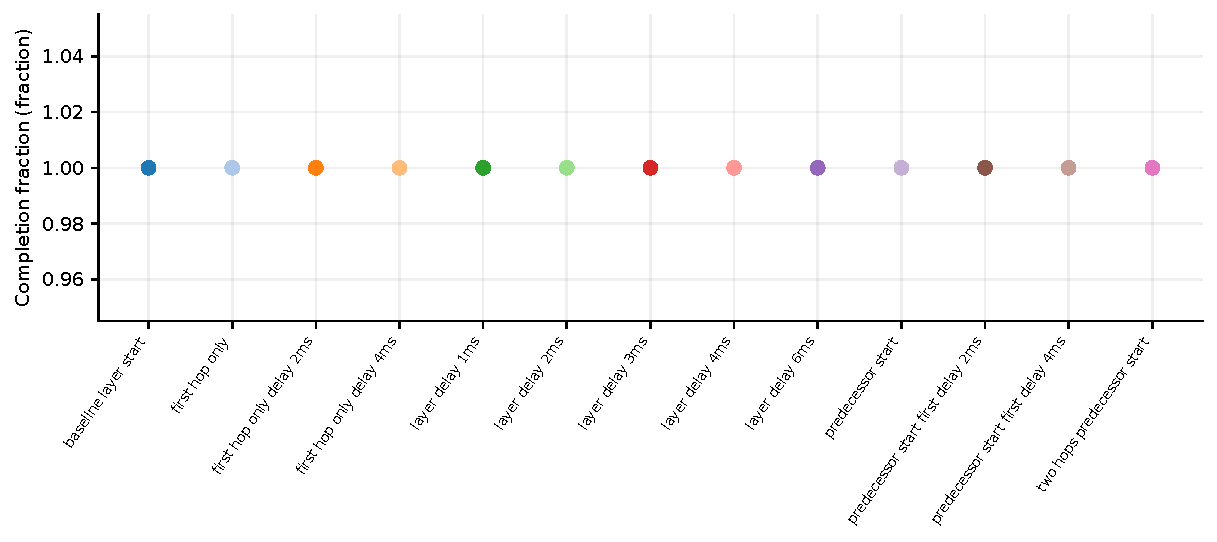
\includegraphics[width=.94\linewidth,height=.31\textheight,keepaspectratio]{figures/variants/mesh_xy_completion_rate.pdf}\captionof{figure}{Thirteen Dynamic launch variants, M=4 and C=3; zero-delay structural rules and delay sensitivities are distinguished in the definitions.}\end{center}
\begin{center}{\scriptsize\setlength{\tabcolsep}{3pt}
\begin{tabular}{lrr}
\toprule
Variant & Mean $\pm$ SD & n \\
\midrule
baseline-layer-start & $1.000\pm0.000$ & 2 \\
first-hop-only & $1.000\pm0.000$ & 2 \\
first-hop-only-delay-2ms & $1.000\pm0.000$ & 2 \\
first-hop-only-delay-4ms & $1.000\pm0.000$ & 2 \\
layer-delay-1ms & $1.000\pm0.000$ & 2 \\
layer-delay-2ms & $1.000\pm0.000$ & 2 \\
layer-delay-3ms & $1.000\pm0.000$ & 2 \\
layer-delay-4ms & $1.000\pm0.000$ & 2 \\
layer-delay-6ms & $1.000\pm0.000$ & 2 \\
predecessor-start & $1.000\pm0.000$ & 2 \\
predecessor-start-first-delay-2ms & $1.000\pm0.000$ & 2 \\
predecessor-start-first-delay-4ms & $1.000\pm0.000$ & 2 \\
two-hops-predecessor-start & $1.000\pm0.000$ & 2 \\
\bottomrule\end{tabular}}
\captionof{table}{All thirteen variants; n counts byte-distinct trace/physics runs, not conceptual aliases.}
{\footnotesize\href{https://github.com/sanjeevkrishnaa/Compiler-Driven-ACE/blob/codex/ace-scheduler-correctness/docs/latex/qft96_final/data/variants_mesh_xy_completion_rate.csv}{Exact CSV values and sample counts}}
\end{center}
\section{Mesh / yx}
\clearpage\subsection*{Mean request latency}
\begin{center}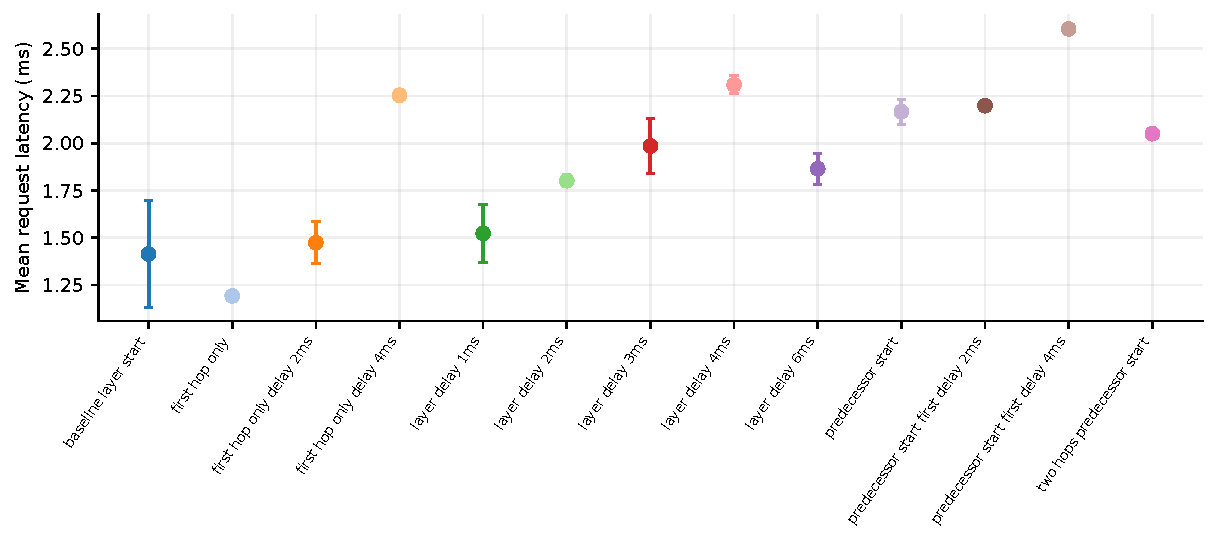
\includegraphics[width=.94\linewidth,height=.31\textheight,keepaspectratio]{figures/variants/mesh_yx_request_latency_mean_ms.pdf}\captionof{figure}{Thirteen Dynamic launch variants, M=4 and C=3; zero-delay structural rules and delay sensitivities are distinguished in the definitions.}\end{center}
\begin{center}{\scriptsize\setlength{\tabcolsep}{3pt}
\begin{tabular}{lrr}
\toprule
Variant & Mean $\pm$ SD & n \\
\midrule
baseline-layer-start & $1.414\pm0.282$ & 2 \\
first-hop-only & $1.192\pm0.025$ & 2 \\
first-hop-only-delay-2ms & $1.474\pm0.110$ & 2 \\
first-hop-only-delay-4ms & $2.254\pm0.016$ & 2 \\
layer-delay-1ms & $1.523\pm0.153$ & 2 \\
layer-delay-2ms & $1.801\pm0.033$ & 2 \\
layer-delay-3ms & $1.985\pm0.146$ & 2 \\
layer-delay-4ms & $2.309\pm0.048$ & 2 \\
layer-delay-6ms & $1.864\pm0.081$ & 2 \\
predecessor-start & $2.166\pm0.066$ & 2 \\
predecessor-start-first-delay-2ms & $2.198\pm0.011$ & 2 \\
predecessor-start-first-delay-4ms & $2.604\pm0.003$ & 2 \\
two-hops-predecessor-start & $2.050\pm0.002$ & 2 \\
\bottomrule\end{tabular}}
\captionof{table}{All thirteen variants; n counts byte-distinct trace/physics runs, not conceptual aliases.}
{\footnotesize\href{https://github.com/sanjeevkrishnaa/Compiler-Driven-ACE/blob/codex/ace-scheduler-correctness/docs/latex/qft96_final/data/variants_mesh_yx_request_latency_mean_ms.csv}{Exact CSV values and sample counts}}
\end{center}
\clearpage\subsection*{Median request latency}
\begin{center}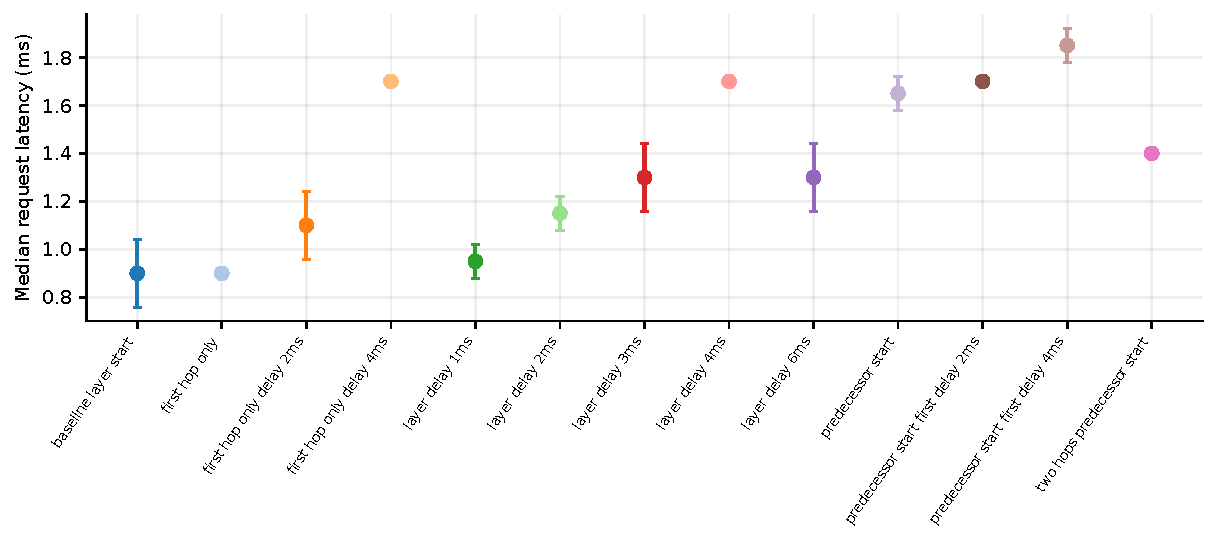
\includegraphics[width=.94\linewidth,height=.31\textheight,keepaspectratio]{figures/variants/mesh_yx_request_latency_median_ms.pdf}\captionof{figure}{Thirteen Dynamic launch variants, M=4 and C=3; zero-delay structural rules and delay sensitivities are distinguished in the definitions.}\end{center}
\begin{center}{\scriptsize\setlength{\tabcolsep}{3pt}
\begin{tabular}{lrr}
\toprule
Variant & Mean $\pm$ SD & n \\
\midrule
baseline-layer-start & $0.9000\pm0.1414$ & 2 \\
first-hop-only & $0.9000\pm0.0000$ & 2 \\
first-hop-only-delay-2ms & $1.100\pm0.141$ & 2 \\
first-hop-only-delay-4ms & $1.700\pm0.000$ & 2 \\
layer-delay-1ms & $0.9500\pm0.0707$ & 2 \\
layer-delay-2ms & $1.150\pm0.071$ & 2 \\
layer-delay-3ms & $1.300\pm0.141$ & 2 \\
layer-delay-4ms & $1.700\pm0.000$ & 2 \\
layer-delay-6ms & $1.300\pm0.141$ & 2 \\
predecessor-start & $1.650\pm0.071$ & 2 \\
predecessor-start-first-delay-2ms & $1.700\pm0.000$ & 2 \\
predecessor-start-first-delay-4ms & $1.850\pm0.071$ & 2 \\
two-hops-predecessor-start & $1.400\pm0.000$ & 2 \\
\bottomrule\end{tabular}}
\captionof{table}{All thirteen variants; n counts byte-distinct trace/physics runs, not conceptual aliases.}
{\footnotesize\href{https://github.com/sanjeevkrishnaa/Compiler-Driven-ACE/blob/codex/ace-scheduler-correctness/docs/latex/qft96_final/data/variants_mesh_yx_request_latency_median_ms.csv}{Exact CSV values and sample counts}}
\end{center}
\clearpage\subsection*{p95 request latency}
\begin{center}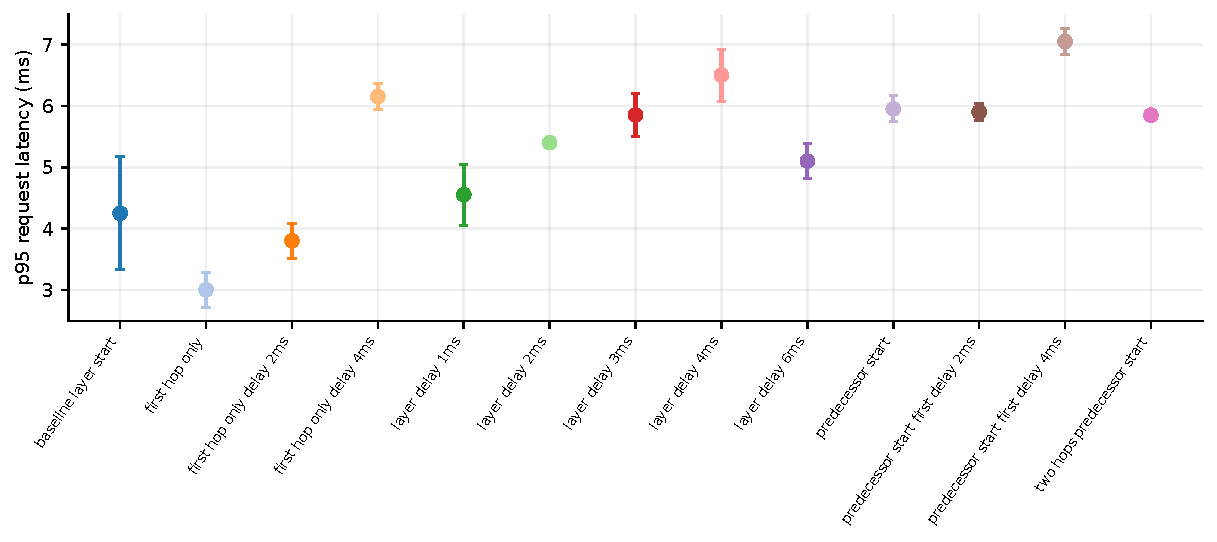
\includegraphics[width=.94\linewidth,height=.31\textheight,keepaspectratio]{figures/variants/mesh_yx_request_latency_p95_ms.pdf}\captionof{figure}{Thirteen Dynamic launch variants, M=4 and C=3; zero-delay structural rules and delay sensitivities are distinguished in the definitions.}\end{center}
\begin{center}{\scriptsize\setlength{\tabcolsep}{3pt}
\begin{tabular}{lrr}
\toprule
Variant & Mean $\pm$ SD & n \\
\midrule
baseline-layer-start & $4.250\pm0.919$ & 2 \\
first-hop-only & $3.000\pm0.283$ & 2 \\
first-hop-only-delay-2ms & $3.800\pm0.283$ & 2 \\
first-hop-only-delay-4ms & $6.150\pm0.212$ & 2 \\
layer-delay-1ms & $4.550\pm0.495$ & 2 \\
layer-delay-2ms & $5.400\pm0.000$ & 2 \\
layer-delay-3ms & $5.850\pm0.354$ & 2 \\
layer-delay-4ms & $6.500\pm0.424$ & 2 \\
layer-delay-6ms & $5.100\pm0.283$ & 2 \\
predecessor-start & $5.950\pm0.212$ & 2 \\
predecessor-start-first-delay-2ms & $5.900\pm0.141$ & 2 \\
predecessor-start-first-delay-4ms & $7.050\pm0.212$ & 2 \\
two-hops-predecessor-start & $5.850\pm0.071$ & 2 \\
\bottomrule\end{tabular}}
\captionof{table}{All thirteen variants; n counts byte-distinct trace/physics runs, not conceptual aliases.}
{\footnotesize\href{https://github.com/sanjeevkrishnaa/Compiler-Driven-ACE/blob/codex/ace-scheduler-correctness/docs/latex/qft96_final/data/variants_mesh_yx_request_latency_p95_ms.csv}{Exact CSV values and sample counts}}
\end{center}
\clearpage\subsection*{Maximum request latency}
\begin{center}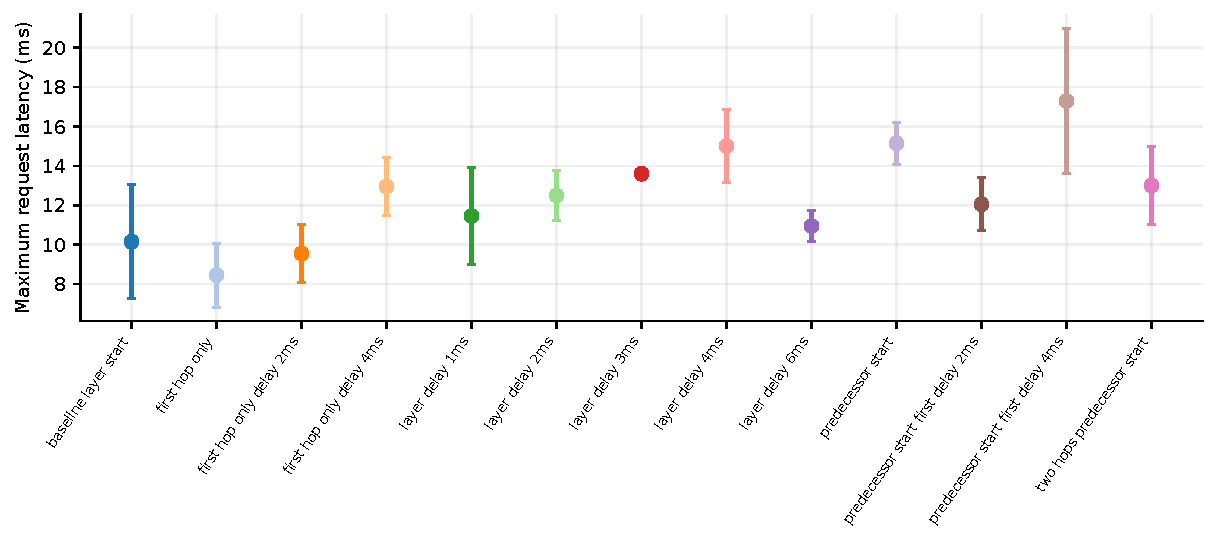
\includegraphics[width=.94\linewidth,height=.31\textheight,keepaspectratio]{figures/variants/mesh_yx_request_latency_max_ms.pdf}\captionof{figure}{Thirteen Dynamic launch variants, M=4 and C=3; zero-delay structural rules and delay sensitivities are distinguished in the definitions.}\end{center}
\begin{center}{\scriptsize\setlength{\tabcolsep}{3pt}
\begin{tabular}{lrr}
\toprule
Variant & Mean $\pm$ SD & n \\
\midrule
baseline-layer-start & $10.150\pm2.899$ & 2 \\
first-hop-only & $8.450\pm1.626$ & 2 \\
first-hop-only-delay-2ms & $9.550\pm1.485$ & 2 \\
first-hop-only-delay-4ms & $12.950\pm1.485$ & 2 \\
layer-delay-1ms & $11.450\pm2.475$ & 2 \\
layer-delay-2ms & $12.500\pm1.273$ & 2 \\
layer-delay-3ms & $13.600\pm0.283$ & 2 \\
layer-delay-4ms & $15.000\pm1.839$ & 2 \\
layer-delay-6ms & $10.950\pm0.778$ & 2 \\
predecessor-start & $15.150\pm1.061$ & 2 \\
predecessor-start-first-delay-2ms & $12.050\pm1.344$ & 2 \\
predecessor-start-first-delay-4ms & $17.300\pm3.677$ & 2 \\
two-hops-predecessor-start & $13.000\pm1.980$ & 2 \\
\bottomrule\end{tabular}}
\captionof{table}{All thirteen variants; n counts byte-distinct trace/physics runs, not conceptual aliases.}
{\footnotesize\href{https://github.com/sanjeevkrishnaa/Compiler-Driven-ACE/blob/codex/ace-scheduler-correctness/docs/latex/qft96_final/data/variants_mesh_yx_request_latency_max_ms.csv}{Exact CSV values and sample counts}}
\end{center}
\clearpage\subsection*{Communication makespan}
\begin{center}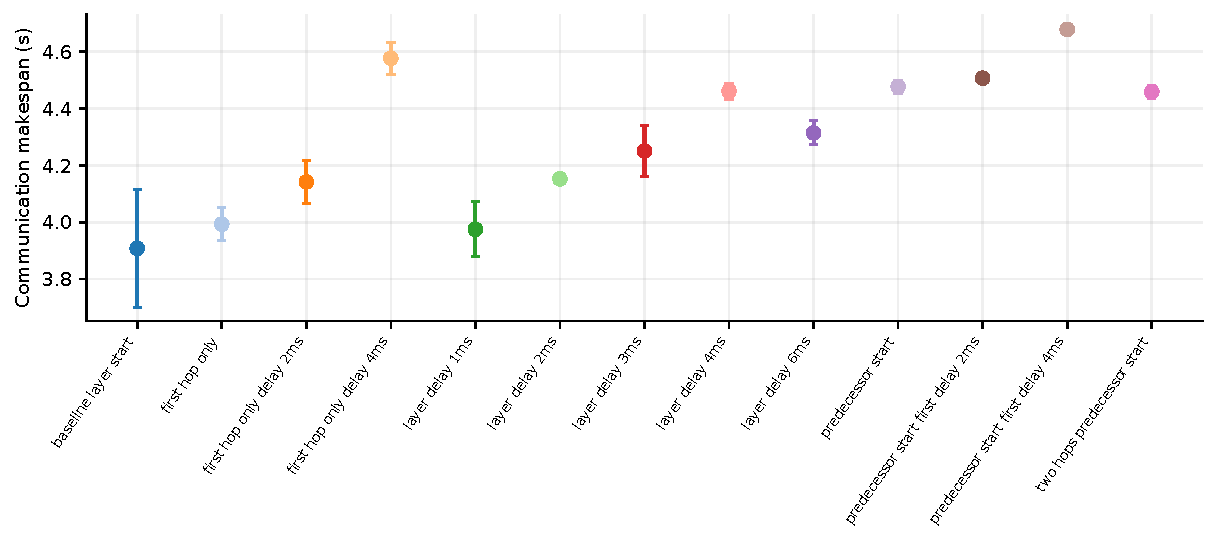
\includegraphics[width=.94\linewidth,height=.31\textheight,keepaspectratio]{figures/variants/mesh_yx_end_to_end_latency_ms.pdf}\captionof{figure}{Thirteen Dynamic launch variants, M=4 and C=3; zero-delay structural rules and delay sensitivities are distinguished in the definitions.}\end{center}
\begin{center}{\scriptsize\setlength{\tabcolsep}{3pt}
\begin{tabular}{lrr}
\toprule
Variant & Mean $\pm$ SD & n \\
\midrule
baseline-layer-start & $3.908\pm0.207$ & 2 \\
first-hop-only & $3.993\pm0.058$ & 2 \\
first-hop-only-delay-2ms & $4.142\pm0.074$ & 2 \\
first-hop-only-delay-4ms & $4.577\pm0.057$ & 2 \\
layer-delay-1ms & $3.975\pm0.097$ & 2 \\
layer-delay-2ms & $4.153\pm0.014$ & 2 \\
layer-delay-3ms & $4.251\pm0.091$ & 2 \\
layer-delay-4ms & $4.462\pm0.028$ & 2 \\
layer-delay-6ms & $4.314\pm0.042$ & 2 \\
predecessor-start & $4.477\pm0.022$ & 2 \\
predecessor-start-first-delay-2ms & $4.507\pm0.003$ & 2 \\
predecessor-start-first-delay-4ms & $4.678\pm0.004$ & 2 \\
two-hops-predecessor-start & $4.459\pm0.022$ & 2 \\
\bottomrule\end{tabular}}
\captionof{table}{All thirteen variants; n counts byte-distinct trace/physics runs, not conceptual aliases.}
{\footnotesize\href{https://github.com/sanjeevkrishnaa/Compiler-Driven-ACE/blob/codex/ace-scheduler-correctness/docs/latex/qft96_final/data/variants_mesh_yx_end_to_end_latency_ms.csv}{Exact CSV values and sample counts}}
\end{center}
\clearpage\subsection*{Mean admission wait}
\begin{center}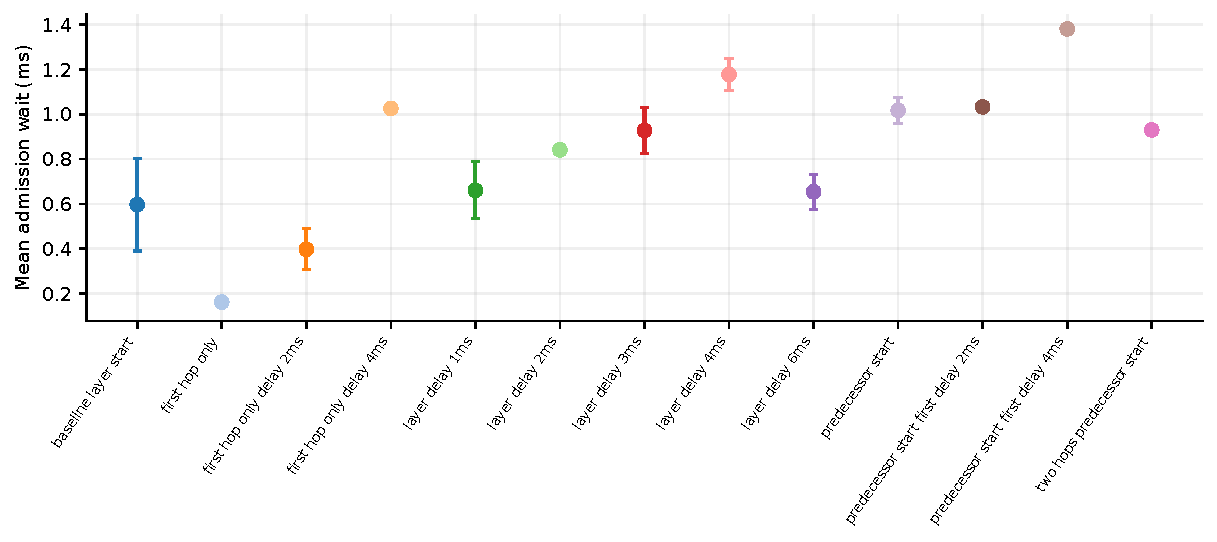
\includegraphics[width=.94\linewidth,height=.31\textheight,keepaspectratio]{figures/variants/mesh_yx_average_admission_wait_ms.pdf}\captionof{figure}{Thirteen Dynamic launch variants, M=4 and C=3; zero-delay structural rules and delay sensitivities are distinguished in the definitions.}\end{center}
\begin{center}{\scriptsize\setlength{\tabcolsep}{3pt}
\begin{tabular}{lrr}
\toprule
Variant & Mean $\pm$ SD & n \\
\midrule
baseline-layer-start & $0.5966\pm0.2069$ & 2 \\
first-hop-only & $0.1613\pm0.0227$ & 2 \\
first-hop-only-delay-2ms & $0.3974\pm0.0908$ & 2 \\
first-hop-only-delay-4ms & $1.026\pm0.022$ & 2 \\
layer-delay-1ms & $0.6602\pm0.1273$ & 2 \\
layer-delay-2ms & $0.8408\pm0.0101$ & 2 \\
layer-delay-3ms & $0.9272\pm0.1035$ & 2 \\
layer-delay-4ms & $1.178\pm0.071$ & 2 \\
layer-delay-6ms & $0.6539\pm0.0788$ & 2 \\
predecessor-start & $1.017\pm0.058$ & 2 \\
predecessor-start-first-delay-2ms & $1.033\pm0.009$ & 2 \\
predecessor-start-first-delay-4ms & $1.381\pm0.002$ & 2 \\
two-hops-predecessor-start & $0.9298\pm0.0019$ & 2 \\
\bottomrule\end{tabular}}
\captionof{table}{All thirteen variants; n counts byte-distinct trace/physics runs, not conceptual aliases.}
{\footnotesize\href{https://github.com/sanjeevkrishnaa/Compiler-Driven-ACE/blob/codex/ace-scheduler-correctness/docs/latex/qft96_final/data/variants_mesh_yx_average_admission_wait_ms.csv}{Exact CSV values and sample counts}}
\end{center}
\clearpage\subsection*{Delivered EPR fidelity}
\begin{center}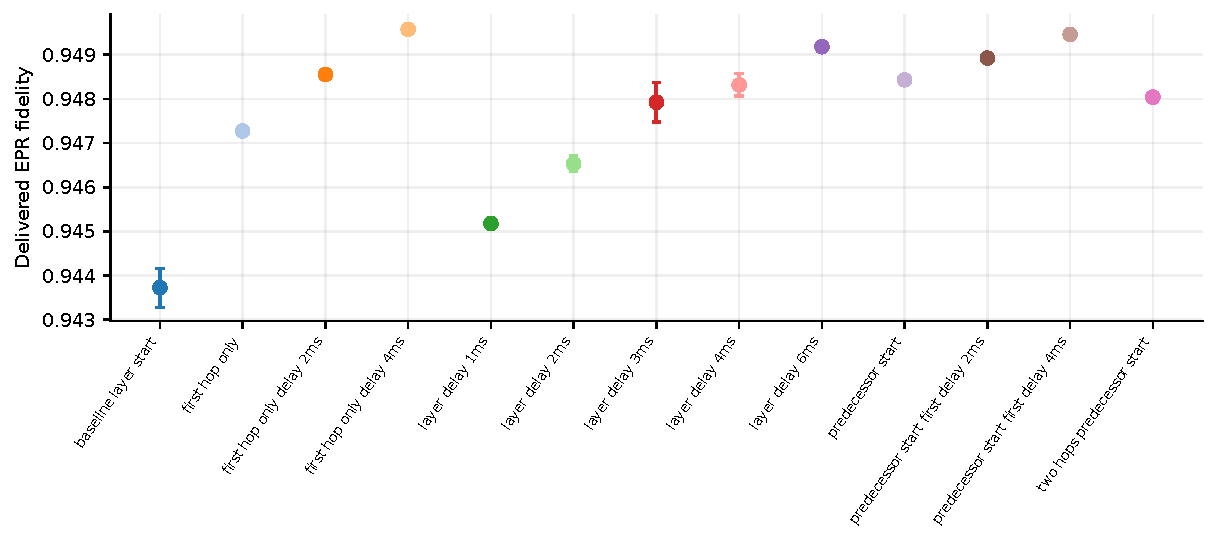
\includegraphics[width=.94\linewidth,height=.31\textheight,keepaspectratio]{figures/variants/mesh_yx_average_delivered_epr_fidelity.pdf}\captionof{figure}{Thirteen Dynamic launch variants, M=4 and C=3; zero-delay structural rules and delay sensitivities are distinguished in the definitions.}\end{center}
\begin{center}{\scriptsize\setlength{\tabcolsep}{3pt}
\begin{tabular}{lrr}
\toprule
Variant & Mean $\pm$ SD & n \\
\midrule
baseline-layer-start & $0.9437\pm0.0004$ & 2 \\
first-hop-only & $0.9473\pm0.0000$ & 2 \\
first-hop-only-delay-2ms & $0.9486\pm0.0001$ & 2 \\
first-hop-only-delay-4ms & $0.9496\pm0.0000$ & 2 \\
layer-delay-1ms & $0.9452\pm0.0000$ & 2 \\
layer-delay-2ms & $0.9465\pm0.0002$ & 2 \\
layer-delay-3ms & $0.9479\pm0.0004$ & 2 \\
layer-delay-4ms & $0.9483\pm0.0003$ & 2 \\
layer-delay-6ms & $0.9492\pm0.0000$ & 2 \\
predecessor-start & $0.9484\pm0.0000$ & 2 \\
predecessor-start-first-delay-2ms & $0.9489\pm0.0000$ & 2 \\
predecessor-start-first-delay-4ms & $0.9495\pm0.0000$ & 2 \\
two-hops-predecessor-start & $0.9480\pm0.0000$ & 2 \\
\bottomrule\end{tabular}}
\captionof{table}{All thirteen variants; n counts byte-distinct trace/physics runs, not conceptual aliases.}
{\footnotesize\href{https://github.com/sanjeevkrishnaa/Compiler-Driven-ACE/blob/codex/ace-scheduler-correctness/docs/latex/qft96_final/data/variants_mesh_yx_average_delivered_epr_fidelity.csv}{Exact CSV values and sample counts}}
\end{center}
\clearpage\subsection*{Compiler readiness fraction}
\begin{center}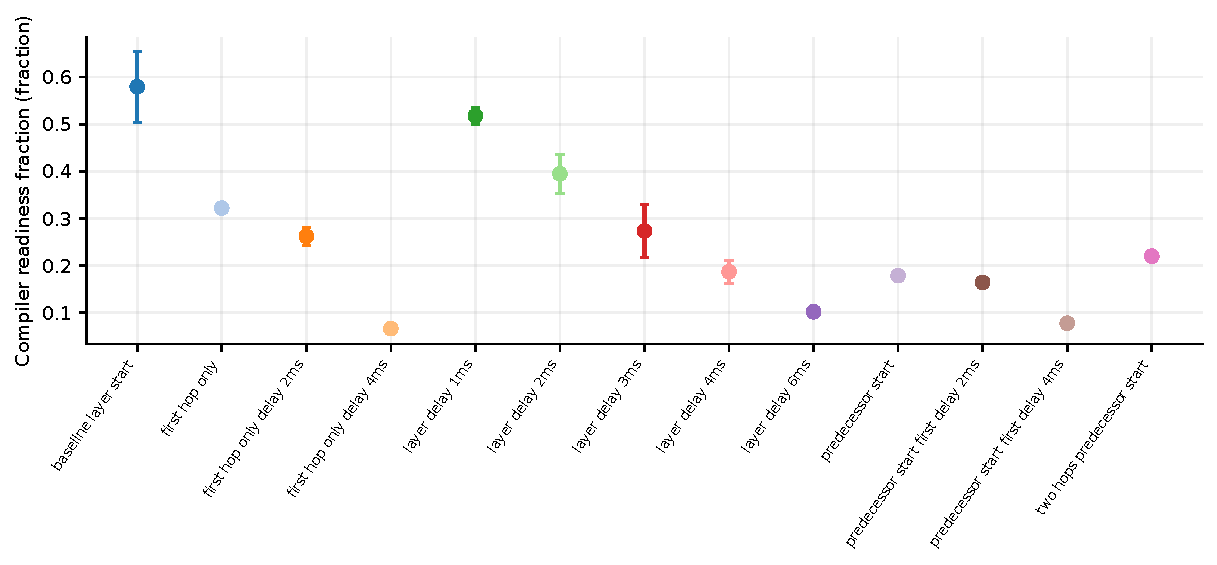
\includegraphics[width=.94\linewidth,height=.31\textheight,keepaspectratio]{figures/variants/mesh_yx_pregenerated_success_rate.pdf}\captionof{figure}{Thirteen Dynamic launch variants, M=4 and C=3; zero-delay structural rules and delay sensitivities are distinguished in the definitions.}\end{center}
\begin{center}{\scriptsize\setlength{\tabcolsep}{3pt}
\begin{tabular}{lrr}
\toprule
Variant & Mean $\pm$ SD & n \\
\midrule
baseline-layer-start & $0.5795\pm0.0752$ & 2 \\
first-hop-only & $0.3219\pm0.0020$ & 2 \\
first-hop-only-delay-2ms & $0.2619\pm0.0193$ & 2 \\
first-hop-only-delay-4ms & $0.0659\pm0.0035$ & 2 \\
layer-delay-1ms & $0.5177\pm0.0173$ & 2 \\
layer-delay-2ms & $0.3945\pm0.0416$ & 2 \\
layer-delay-3ms & $0.2732\pm0.0562$ & 2 \\
layer-delay-4ms & $0.1864\pm0.0243$ & 2 \\
layer-delay-6ms & $0.1017\pm0.0044$ & 2 \\
predecessor-start & $0.1783\pm0.0036$ & 2 \\
predecessor-start-first-delay-2ms & $0.1640\pm0.0016$ & 2 \\
predecessor-start-first-delay-4ms & $0.0773\pm0.0009$ & 2 \\
two-hops-predecessor-start & $0.2198\pm0.0102$ & 2 \\
\bottomrule\end{tabular}}
\captionof{table}{All thirteen variants; n counts byte-distinct trace/physics runs, not conceptual aliases.}
{\footnotesize\href{https://github.com/sanjeevkrishnaa/Compiler-Driven-ACE/blob/codex/ace-scheduler-correctness/docs/latex/qft96_final/data/variants_mesh_yx_pregenerated_success_rate.csv}{Exact CSV values and sample counts}}
\end{center}
\clearpage\subsection*{Intended compiler-hit fraction}
\begin{center}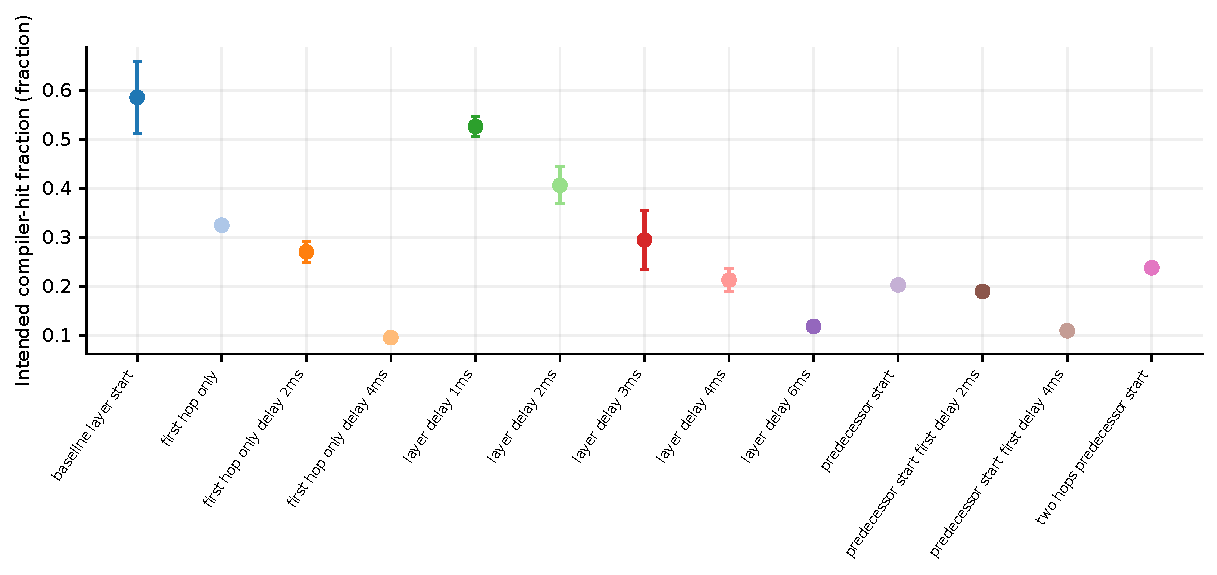
\includegraphics[width=.94\linewidth,height=.31\textheight,keepaspectratio]{figures/variants/mesh_yx_intended_request_hit_rate.pdf}\captionof{figure}{Thirteen Dynamic launch variants, M=4 and C=3; zero-delay structural rules and delay sensitivities are distinguished in the definitions.}\end{center}
\begin{center}{\scriptsize\setlength{\tabcolsep}{3pt}
\begin{tabular}{lrr}
\toprule
Variant & Mean $\pm$ SD & n \\
\midrule
baseline-layer-start & $0.5857\pm0.0733$ & 2 \\
first-hop-only & $0.3246\pm0.0007$ & 2 \\
first-hop-only-delay-2ms & $0.2703\pm0.0213$ & 2 \\
first-hop-only-delay-4ms & $0.0951\pm0.0053$ & 2 \\
layer-delay-1ms & $0.5262\pm0.0195$ & 2 \\
layer-delay-2ms & $0.4062\pm0.0374$ & 2 \\
layer-delay-3ms & $0.2948\pm0.0600$ & 2 \\
layer-delay-4ms & $0.2127\pm0.0243$ & 2 \\
layer-delay-6ms & $0.1182\pm0.0029$ & 2 \\
predecessor-start & $0.2027\pm0.0057$ & 2 \\
predecessor-start-first-delay-2ms & $0.1894\pm0.0000$ & 2 \\
predecessor-start-first-delay-4ms & $0.1090\pm0.0024$ & 2 \\
two-hops-predecessor-start & $0.2376\pm0.0095$ & 2 \\
\bottomrule\end{tabular}}
\captionof{table}{All thirteen variants; n counts byte-distinct trace/physics runs, not conceptual aliases.}
{\footnotesize\href{https://github.com/sanjeevkrishnaa/Compiler-Driven-ACE/blob/codex/ace-scheduler-correctness/docs/latex/qft96_final/data/variants_mesh_yx_intended_request_hit_rate.csv}{Exact CSV values and sample counts}}
\end{center}
\clearpage\subsection*{Compiler fallback fraction}
\begin{center}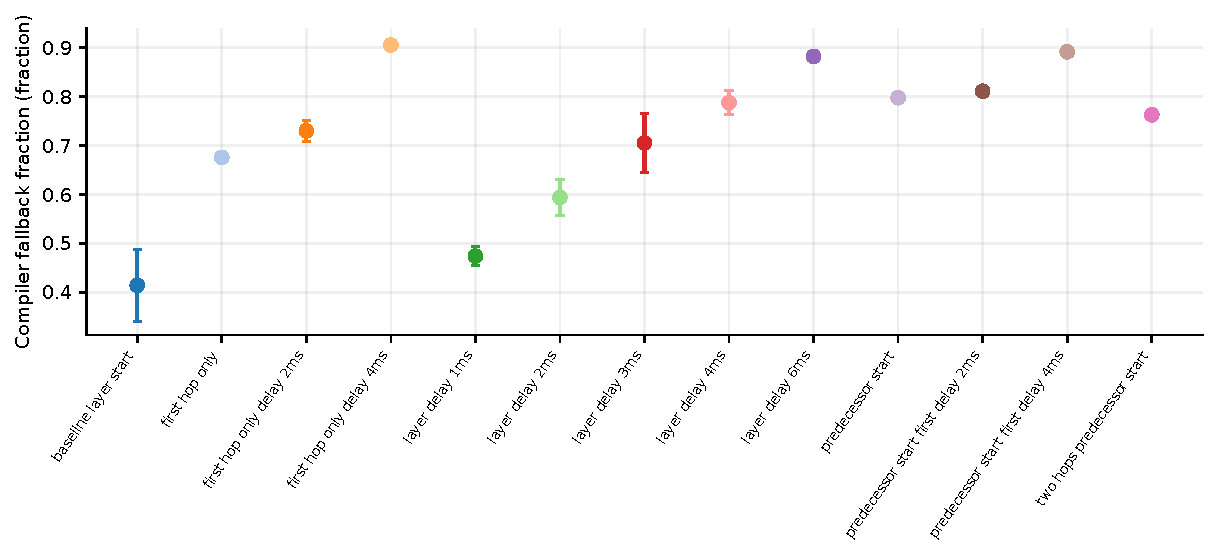
\includegraphics[width=.94\linewidth,height=.31\textheight,keepaspectratio]{figures/variants/mesh_yx_on_demand_fallback_rate.pdf}\captionof{figure}{Thirteen Dynamic launch variants, M=4 and C=3; zero-delay structural rules and delay sensitivities are distinguished in the definitions.}\end{center}
\begin{center}{\scriptsize\setlength{\tabcolsep}{3pt}
\begin{tabular}{lrr}
\toprule
Variant & Mean $\pm$ SD & n \\
\midrule
baseline-layer-start & $0.4143\pm0.0733$ & 2 \\
first-hop-only & $0.6754\pm0.0007$ & 2 \\
first-hop-only-delay-2ms & $0.7297\pm0.0213$ & 2 \\
first-hop-only-delay-4ms & $0.9049\pm0.0053$ & 2 \\
layer-delay-1ms & $0.4738\pm0.0195$ & 2 \\
layer-delay-2ms & $0.5938\pm0.0374$ & 2 \\
layer-delay-3ms & $0.7052\pm0.0600$ & 2 \\
layer-delay-4ms & $0.7873\pm0.0243$ & 2 \\
layer-delay-6ms & $0.8818\pm0.0029$ & 2 \\
predecessor-start & $0.7973\pm0.0057$ & 2 \\
predecessor-start-first-delay-2ms & $0.8106\pm0.0000$ & 2 \\
predecessor-start-first-delay-4ms & $0.8910\pm0.0024$ & 2 \\
two-hops-predecessor-start & $0.7624\pm0.0095$ & 2 \\
\bottomrule\end{tabular}}
\captionof{table}{All thirteen variants; n counts byte-distinct trace/physics runs, not conceptual aliases.}
{\footnotesize\href{https://github.com/sanjeevkrishnaa/Compiler-Driven-ACE/blob/codex/ace-scheduler-correctness/docs/latex/qft96_final/data/variants_mesh_yx_on_demand_fallback_rate.csv}{Exact CSV values and sample counts}}
\end{center}
\clearpage\subsection*{Compiler-cache waste}
\begin{center}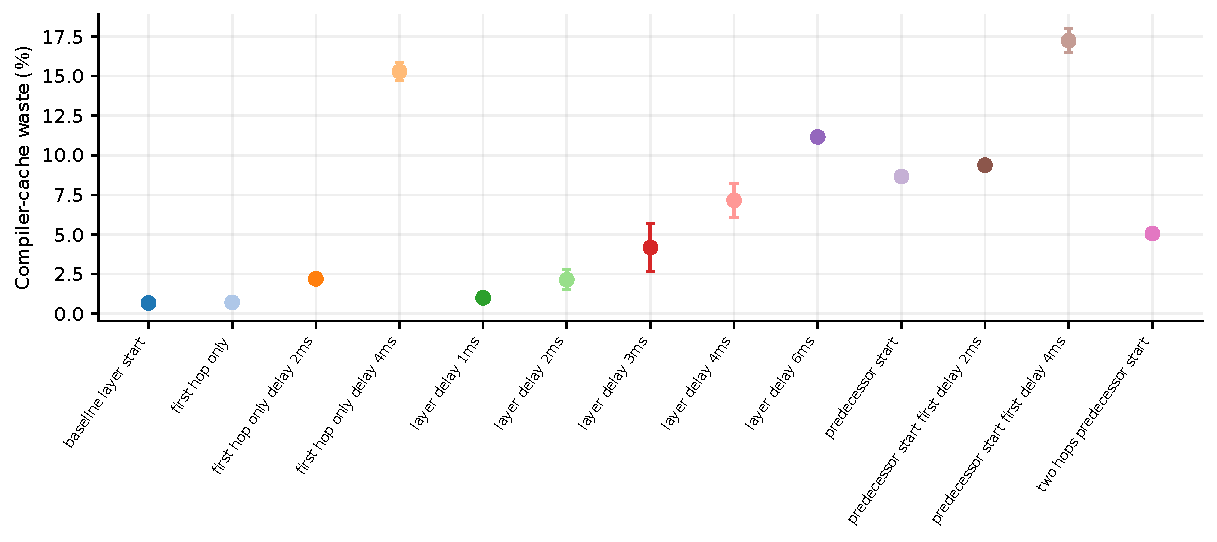
\includegraphics[width=.94\linewidth,height=.31\textheight,keepaspectratio]{figures/variants/mesh_yx_compiler_waste_percentage.pdf}\captionof{figure}{Thirteen Dynamic launch variants, M=4 and C=3; zero-delay structural rules and delay sensitivities are distinguished in the definitions.}\end{center}
\begin{center}{\scriptsize\setlength{\tabcolsep}{3pt}
\begin{tabular}{lrr}
\toprule
Variant & Mean $\pm$ SD & n \\
\midrule
baseline-layer-start & $0.6729\pm0.2681$ & 2 \\
first-hop-only & $0.7103\pm0.0016$ & 2 \\
first-hop-only-delay-2ms & $2.198\pm0.105$ & 2 \\
first-hop-only-delay-4ms & $15.302\pm0.584$ & 2 \\
layer-delay-1ms & $0.9976\pm0.1386$ & 2 \\
layer-delay-2ms & $2.140\pm0.623$ & 2 \\
layer-delay-3ms & $4.173\pm1.498$ & 2 \\
layer-delay-4ms & $7.153\pm1.054$ & 2 \\
layer-delay-6ms & $11.158\pm0.367$ & 2 \\
predecessor-start & $8.666\pm0.296$ & 2 \\
predecessor-start-first-delay-2ms & $9.382\pm0.316$ & 2 \\
predecessor-start-first-delay-4ms & $17.243\pm0.769$ & 2 \\
two-hops-predecessor-start & $5.058\pm0.330$ & 2 \\
\bottomrule\end{tabular}}
\captionof{table}{All thirteen variants; n counts byte-distinct trace/physics runs, not conceptual aliases.}
{\footnotesize\href{https://github.com/sanjeevkrishnaa/Compiler-Driven-ACE/blob/codex/ace-scheduler-correctness/docs/latex/qft96_final/data/variants_mesh_yx_compiler_waste_percentage.csv}{Exact CSV values and sample counts}}
\end{center}
\clearpage\subsection*{Native-protocol waste}
\begin{center}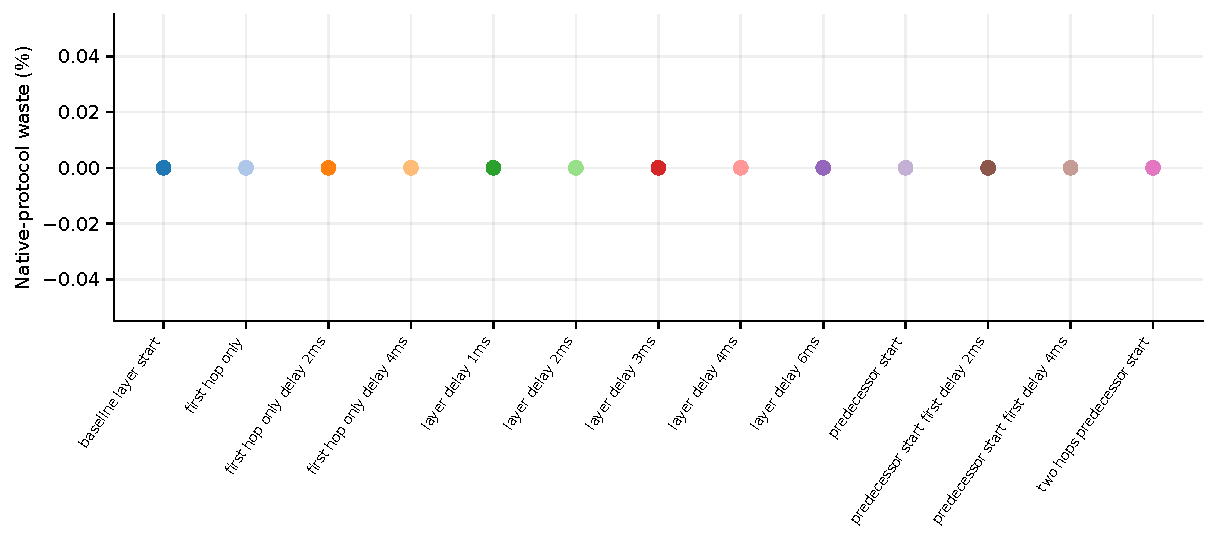
\includegraphics[width=.94\linewidth,height=.31\textheight,keepaspectratio]{figures/variants/mesh_yx_protocol_waste_percentage.pdf}\captionof{figure}{Thirteen Dynamic launch variants, M=4 and C=3; zero-delay structural rules and delay sensitivities are distinguished in the definitions.}\end{center}
\begin{center}{\scriptsize\setlength{\tabcolsep}{3pt}
\begin{tabular}{lrr}
\toprule
Variant & Mean $\pm$ SD & n \\
\midrule
baseline-layer-start & $0.0000\pm0.0000$ & 2 \\
first-hop-only & $0.0000\pm0.0000$ & 2 \\
first-hop-only-delay-2ms & $0.0000\pm0.0000$ & 2 \\
first-hop-only-delay-4ms & $0.0000\pm0.0000$ & 2 \\
layer-delay-1ms & $0.0000\pm0.0000$ & 2 \\
layer-delay-2ms & $0.0000\pm0.0000$ & 2 \\
layer-delay-3ms & $0.0000\pm0.0000$ & 2 \\
layer-delay-4ms & $0.0000\pm0.0000$ & 2 \\
layer-delay-6ms & $0.0000\pm0.0000$ & 2 \\
predecessor-start & $0.0000\pm0.0000$ & 2 \\
predecessor-start-first-delay-2ms & $0.0000\pm0.0000$ & 2 \\
predecessor-start-first-delay-4ms & $0.0000\pm0.0000$ & 2 \\
two-hops-predecessor-start & $0.0000\pm0.0000$ & 2 \\
\bottomrule\end{tabular}}
\captionof{table}{All thirteen variants; n counts byte-distinct trace/physics runs, not conceptual aliases.}
{\footnotesize\href{https://github.com/sanjeevkrishnaa/Compiler-Driven-ACE/blob/codex/ace-scheduler-correctness/docs/latex/qft96_final/data/variants_mesh_yx_protocol_waste_percentage.csv}{Exact CSV values and sample counts}}
\end{center}
\clearpage\subsection*{Compiler-pair expiry}
\begin{center}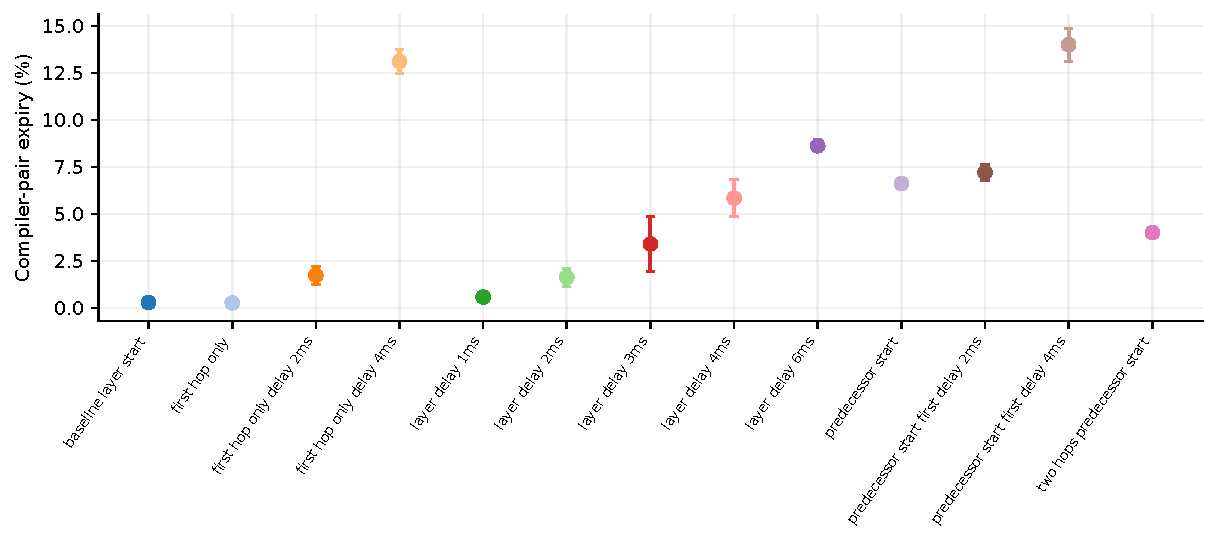
\includegraphics[width=.94\linewidth,height=.31\textheight,keepaspectratio]{figures/variants/mesh_yx_compiler_expiry_percentage.pdf}\captionof{figure}{Thirteen Dynamic launch variants, M=4 and C=3; zero-delay structural rules and delay sensitivities are distinguished in the definitions.}\end{center}
\begin{center}{\scriptsize\setlength{\tabcolsep}{3pt}
\begin{tabular}{lrr}
\toprule
Variant & Mean $\pm$ SD & n \\
\midrule
baseline-layer-start & $0.3000\pm0.2534$ & 2 \\
first-hop-only & $0.2763\pm0.0564$ & 2 \\
first-hop-only-delay-2ms & $1.746\pm0.466$ & 2 \\
first-hop-only-delay-4ms & $13.119\pm0.640$ & 2 \\
layer-delay-1ms & $0.5866\pm0.2269$ & 2 \\
layer-delay-2ms & $1.638\pm0.492$ & 2 \\
layer-delay-3ms & $3.415\pm1.474$ & 2 \\
layer-delay-4ms & $5.854\pm1.000$ & 2 \\
layer-delay-6ms & $8.636\pm0.315$ & 2 \\
predecessor-start & $6.630\pm0.164$ & 2 \\
predecessor-start-first-delay-2ms & $7.222\pm0.411$ & 2 \\
predecessor-start-first-delay-4ms & $14.011\pm0.867$ & 2 \\
two-hops-predecessor-start & $4.021\pm0.001$ & 2 \\
\bottomrule\end{tabular}}
\captionof{table}{All thirteen variants; n counts byte-distinct trace/physics runs, not conceptual aliases.}
{\footnotesize\href{https://github.com/sanjeevkrishnaa/Compiler-Driven-ACE/blob/codex/ace-scheduler-correctness/docs/latex/qft96_final/data/variants_mesh_yx_compiler_expiry_percentage.csv}{Exact CSV values and sample counts}}
\end{center}
\clearpage\subsection*{Used compiler-pair storage time}
\begin{center}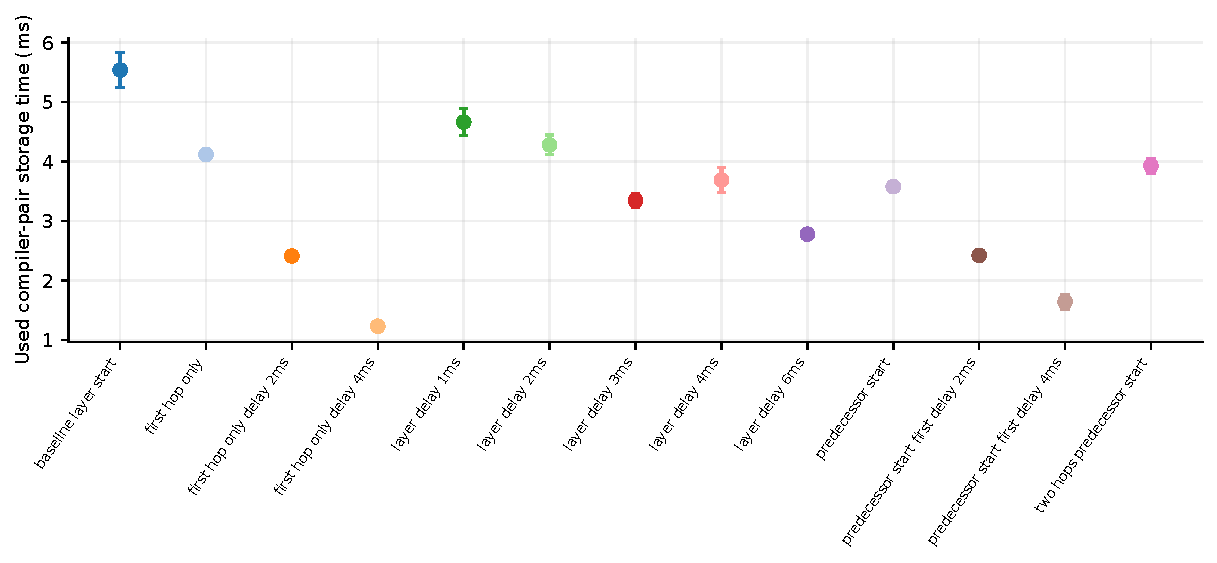
\includegraphics[width=.94\linewidth,height=.31\textheight,keepaspectratio]{figures/variants/mesh_yx_average_storage_time_ms.pdf}\captionof{figure}{Thirteen Dynamic launch variants, M=4 and C=3; zero-delay structural rules and delay sensitivities are distinguished in the definitions.}\end{center}
\begin{center}{\scriptsize\setlength{\tabcolsep}{3pt}
\begin{tabular}{lrr}
\toprule
Variant & Mean $\pm$ SD & n \\
\midrule
baseline-layer-start & $5.539\pm0.301$ & 2 \\
first-hop-only & $4.118\pm0.008$ & 2 \\
first-hop-only-delay-2ms & $2.411\pm0.047$ & 2 \\
first-hop-only-delay-4ms & $1.229\pm0.035$ & 2 \\
layer-delay-1ms & $4.664\pm0.229$ & 2 \\
layer-delay-2ms & $4.279\pm0.167$ & 2 \\
layer-delay-3ms & $3.345\pm0.120$ & 2 \\
layer-delay-4ms & $3.689\pm0.206$ & 2 \\
layer-delay-6ms & $2.778\pm0.048$ & 2 \\
predecessor-start & $3.577\pm0.005$ & 2 \\
predecessor-start-first-delay-2ms & $2.422\pm0.008$ & 2 \\
predecessor-start-first-delay-4ms & $1.639\pm0.121$ & 2 \\
two-hops-predecessor-start & $3.926\pm0.125$ & 2 \\
\bottomrule\end{tabular}}
\captionof{table}{All thirteen variants; n counts byte-distinct trace/physics runs, not conceptual aliases.}
{\footnotesize\href{https://github.com/sanjeevkrishnaa/Compiler-Driven-ACE/blob/codex/ace-scheduler-correctness/docs/latex/qft96_final/data/variants_mesh_yx_average_storage_time_ms.csv}{Exact CSV values and sample counts}}
\end{center}
\clearpage\subsection*{Delivered-hop throughput}
\begin{center}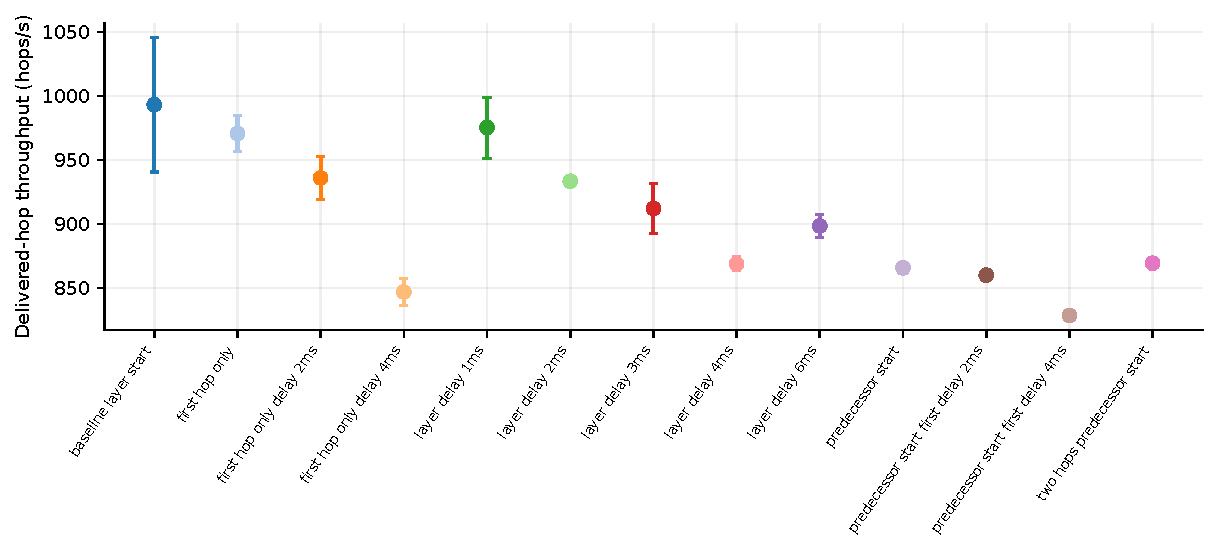
\includegraphics[width=.94\linewidth,height=.31\textheight,keepaspectratio]{figures/variants/mesh_yx_hop_throughput_s.pdf}\captionof{figure}{Thirteen Dynamic launch variants, M=4 and C=3; zero-delay structural rules and delay sensitivities are distinguished in the definitions.}\end{center}
\begin{center}{\scriptsize\setlength{\tabcolsep}{3pt}
\begin{tabular}{lrr}
\toprule
Variant & Mean $\pm$ SD & n \\
\midrule
baseline-layer-start & $993.15\pm52.58$ & 2 \\
first-hop-only & $970.68\pm14.08$ & 2 \\
first-hop-only-delay-2ms & $935.96\pm16.76$ & 2 \\
first-hop-only-delay-4ms & $846.89\pm10.48$ & 2 \\
layer-delay-1ms & $975.31\pm23.84$ & 2 \\
layer-delay-2ms & $933.40\pm3.13$ & 2 \\
layer-delay-3ms & $912.09\pm19.42$ & 2 \\
layer-delay-4ms & $868.77\pm5.47$ & 2 \\
layer-delay-6ms & $898.42\pm8.77$ & 2 \\
predecessor-start & $865.73\pm4.33$ & 2 \\
predecessor-start-first-delay-2ms & $860.01\pm0.59$ & 2 \\
predecessor-start-first-delay-4ms & $828.52\pm0.62$ & 2 \\
two-hops-predecessor-start & $869.30\pm4.26$ & 2 \\
\bottomrule\end{tabular}}
\captionof{table}{All thirteen variants; n counts byte-distinct trace/physics runs, not conceptual aliases.}
{\footnotesize\href{https://github.com/sanjeevkrishnaa/Compiler-Driven-ACE/blob/codex/ace-scheduler-correctness/docs/latex/qft96_final/data/variants_mesh_yx_hop_throughput_s.csv}{Exact CSV values and sample counts}}
\end{center}
\clearpage\subsection*{Completion fraction}
\begin{center}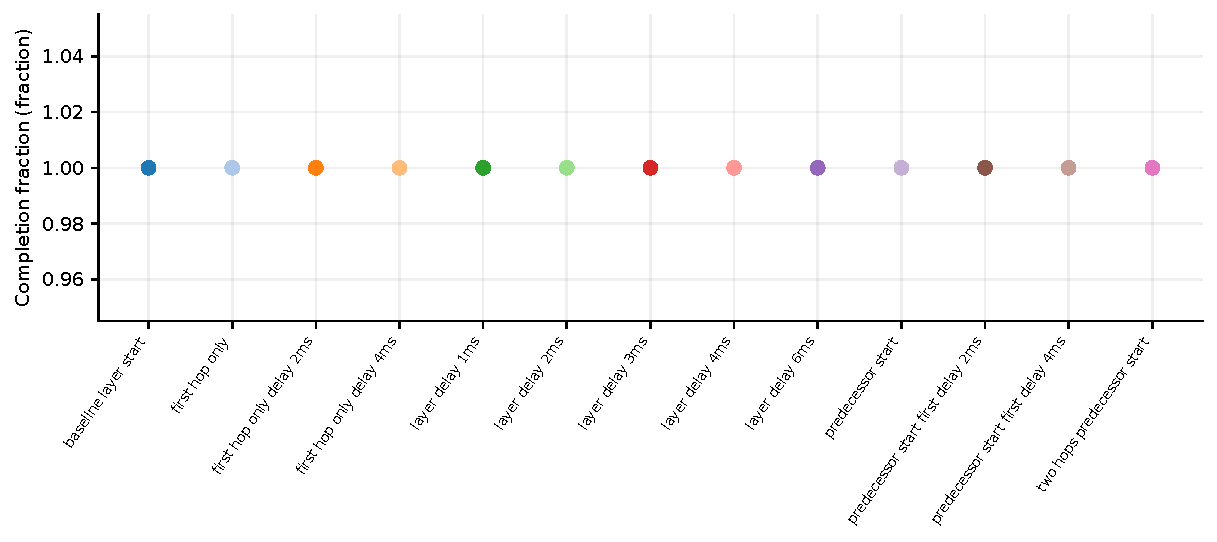
\includegraphics[width=.94\linewidth,height=.31\textheight,keepaspectratio]{figures/variants/mesh_yx_completion_rate.pdf}\captionof{figure}{Thirteen Dynamic launch variants, M=4 and C=3; zero-delay structural rules and delay sensitivities are distinguished in the definitions.}\end{center}
\begin{center}{\scriptsize\setlength{\tabcolsep}{3pt}
\begin{tabular}{lrr}
\toprule
Variant & Mean $\pm$ SD & n \\
\midrule
baseline-layer-start & $1.000\pm0.000$ & 2 \\
first-hop-only & $1.000\pm0.000$ & 2 \\
first-hop-only-delay-2ms & $1.000\pm0.000$ & 2 \\
first-hop-only-delay-4ms & $1.000\pm0.000$ & 2 \\
layer-delay-1ms & $1.000\pm0.000$ & 2 \\
layer-delay-2ms & $1.000\pm0.000$ & 2 \\
layer-delay-3ms & $1.000\pm0.000$ & 2 \\
layer-delay-4ms & $1.000\pm0.000$ & 2 \\
layer-delay-6ms & $1.000\pm0.000$ & 2 \\
predecessor-start & $1.000\pm0.000$ & 2 \\
predecessor-start-first-delay-2ms & $1.000\pm0.000$ & 2 \\
predecessor-start-first-delay-4ms & $1.000\pm0.000$ & 2 \\
two-hops-predecessor-start & $1.000\pm0.000$ & 2 \\
\bottomrule\end{tabular}}
\captionof{table}{All thirteen variants; n counts byte-distinct trace/physics runs, not conceptual aliases.}
{\footnotesize\href{https://github.com/sanjeevkrishnaa/Compiler-Driven-ACE/blob/codex/ace-scheduler-correctness/docs/latex/qft96_final/data/variants_mesh_yx_completion_rate.csv}{Exact CSV values and sample counts}}
\end{center}
\section{Mesh / shortest\_reliable}
\clearpage\subsection*{Mean request latency}
\begin{center}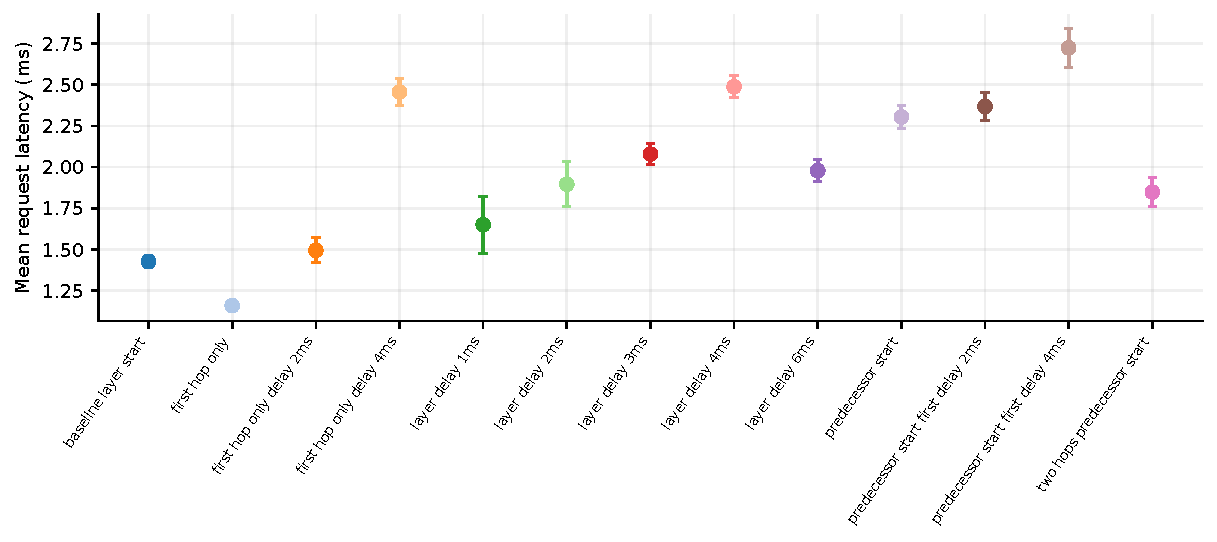
\includegraphics[width=.94\linewidth,height=.31\textheight,keepaspectratio]{figures/variants/mesh_shortest_reliable_request_latency_mean_ms.pdf}\captionof{figure}{Thirteen Dynamic launch variants, M=4 and C=3; zero-delay structural rules and delay sensitivities are distinguished in the definitions.}\end{center}
\begin{center}{\scriptsize\setlength{\tabcolsep}{3pt}
\begin{tabular}{lrr}
\toprule
Variant & Mean $\pm$ SD & n \\
\midrule
baseline-layer-start & $1.427\pm0.036$ & 6 \\
first-hop-only & $1.160\pm0.010$ & 6 \\
first-hop-only-delay-2ms & $1.494\pm0.076$ & 6 \\
first-hop-only-delay-4ms & $2.456\pm0.080$ & 6 \\
layer-delay-1ms & $1.650\pm0.173$ & 6 \\
layer-delay-2ms & $1.897\pm0.136$ & 6 \\
layer-delay-3ms & $2.079\pm0.063$ & 6 \\
layer-delay-4ms & $2.487\pm0.066$ & 6 \\
layer-delay-6ms & $1.979\pm0.066$ & 6 \\
predecessor-start & $2.304\pm0.072$ & 6 \\
predecessor-start-first-delay-2ms & $2.368\pm0.087$ & 6 \\
predecessor-start-first-delay-4ms & $2.723\pm0.118$ & 6 \\
two-hops-predecessor-start & $1.849\pm0.088$ & 6 \\
\bottomrule\end{tabular}}
\captionof{table}{All thirteen variants; n counts byte-distinct trace/physics runs, not conceptual aliases.}
{\footnotesize\href{https://github.com/sanjeevkrishnaa/Compiler-Driven-ACE/blob/codex/ace-scheduler-correctness/docs/latex/qft96_final/data/variants_mesh_shortest_reliable_request_latency_mean_ms.csv}{Exact CSV values and sample counts}}
\end{center}
\clearpage\subsection*{Median request latency}
\begin{center}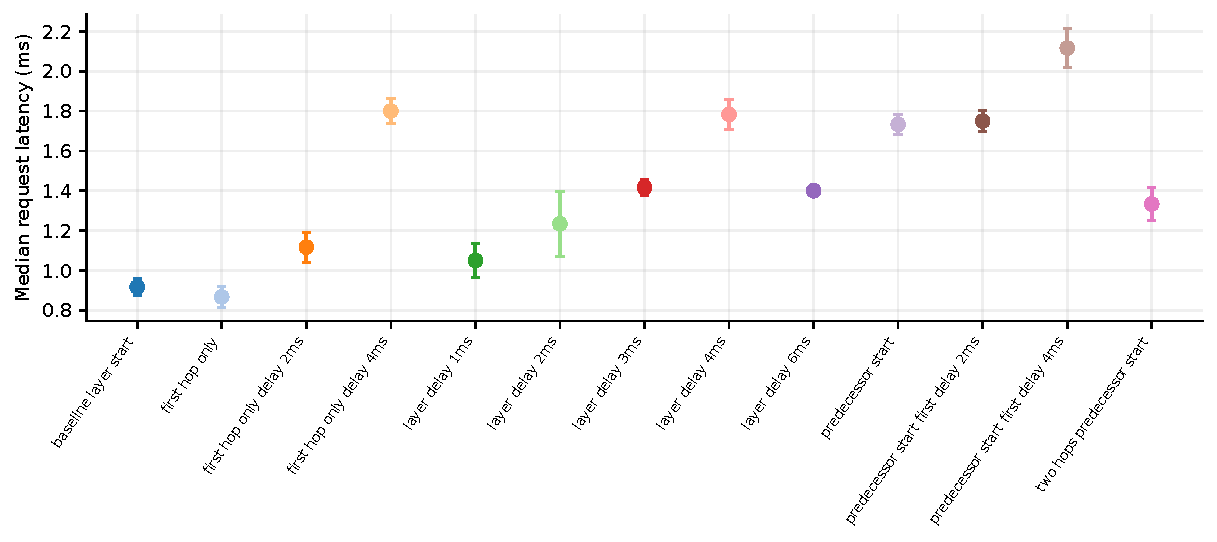
\includegraphics[width=.94\linewidth,height=.31\textheight,keepaspectratio]{figures/variants/mesh_shortest_reliable_request_latency_median_ms.pdf}\captionof{figure}{Thirteen Dynamic launch variants, M=4 and C=3; zero-delay structural rules and delay sensitivities are distinguished in the definitions.}\end{center}
\begin{center}{\scriptsize\setlength{\tabcolsep}{3pt}
\begin{tabular}{lrr}
\toprule
Variant & Mean $\pm$ SD & n \\
\midrule
baseline-layer-start & $0.9167\pm0.0408$ & 6 \\
first-hop-only & $0.8667\pm0.0516$ & 6 \\
first-hop-only-delay-2ms & $1.117\pm0.075$ & 6 \\
first-hop-only-delay-4ms & $1.800\pm0.063$ & 6 \\
layer-delay-1ms & $1.050\pm0.084$ & 6 \\
layer-delay-2ms & $1.233\pm0.163$ & 6 \\
layer-delay-3ms & $1.417\pm0.041$ & 6 \\
layer-delay-4ms & $1.783\pm0.075$ & 6 \\
layer-delay-6ms & $1.400\pm0.000$ & 6 \\
predecessor-start & $1.733\pm0.052$ & 6 \\
predecessor-start-first-delay-2ms & $1.750\pm0.055$ & 6 \\
predecessor-start-first-delay-4ms & $2.117\pm0.098$ & 6 \\
two-hops-predecessor-start & $1.333\pm0.082$ & 6 \\
\bottomrule\end{tabular}}
\captionof{table}{All thirteen variants; n counts byte-distinct trace/physics runs, not conceptual aliases.}
{\footnotesize\href{https://github.com/sanjeevkrishnaa/Compiler-Driven-ACE/blob/codex/ace-scheduler-correctness/docs/latex/qft96_final/data/variants_mesh_shortest_reliable_request_latency_median_ms.csv}{Exact CSV values and sample counts}}
\end{center}
\clearpage\subsection*{p95 request latency}
\begin{center}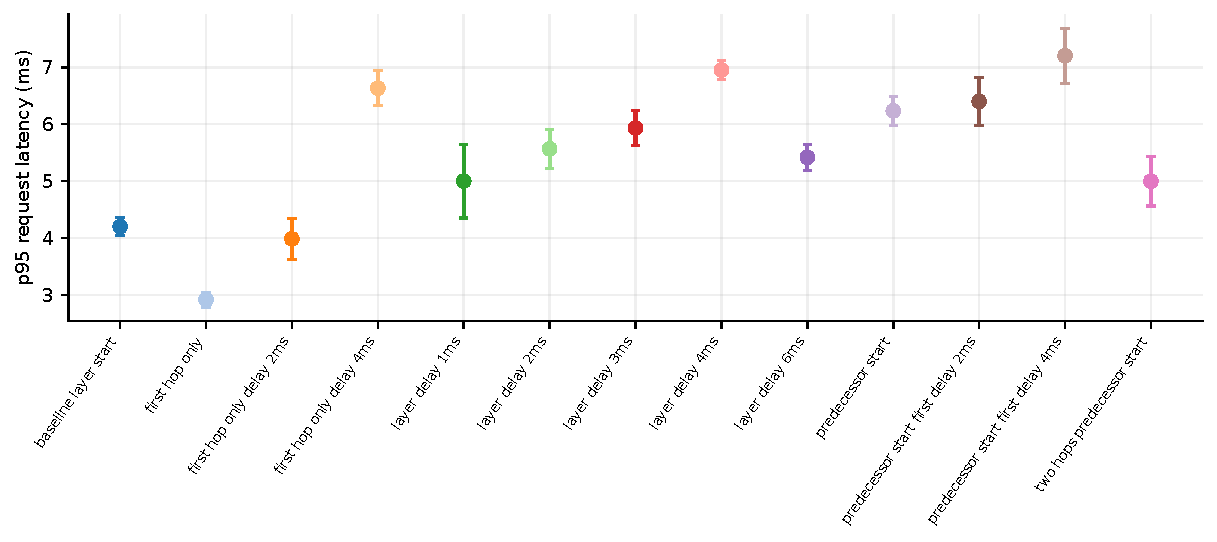
\includegraphics[width=.94\linewidth,height=.31\textheight,keepaspectratio]{figures/variants/mesh_shortest_reliable_request_latency_p95_ms.pdf}\captionof{figure}{Thirteen Dynamic launch variants, M=4 and C=3; zero-delay structural rules and delay sensitivities are distinguished in the definitions.}\end{center}
\begin{center}{\scriptsize\setlength{\tabcolsep}{3pt}
\begin{tabular}{lrr}
\toprule
Variant & Mean $\pm$ SD & n \\
\midrule
baseline-layer-start & $4.200\pm0.155$ & 6 \\
first-hop-only & $2.917\pm0.133$ & 6 \\
first-hop-only-delay-2ms & $3.983\pm0.355$ & 6 \\
first-hop-only-delay-4ms & $6.633\pm0.308$ & 6 \\
layer-delay-1ms & $5.000\pm0.648$ & 6 \\
layer-delay-2ms & $5.567\pm0.339$ & 6 \\
layer-delay-3ms & $5.933\pm0.301$ & 6 \\
layer-delay-4ms & $6.950\pm0.164$ & 6 \\
layer-delay-6ms & $5.417\pm0.232$ & 6 \\
predecessor-start & $6.233\pm0.258$ & 6 \\
predecessor-start-first-delay-2ms & $6.400\pm0.424$ & 6 \\
predecessor-start-first-delay-4ms & $7.200\pm0.482$ & 6 \\
two-hops-predecessor-start & $5.000\pm0.438$ & 6 \\
\bottomrule\end{tabular}}
\captionof{table}{All thirteen variants; n counts byte-distinct trace/physics runs, not conceptual aliases.}
{\footnotesize\href{https://github.com/sanjeevkrishnaa/Compiler-Driven-ACE/blob/codex/ace-scheduler-correctness/docs/latex/qft96_final/data/variants_mesh_shortest_reliable_request_latency_p95_ms.csv}{Exact CSV values and sample counts}}
\end{center}
\clearpage\subsection*{Maximum request latency}
\begin{center}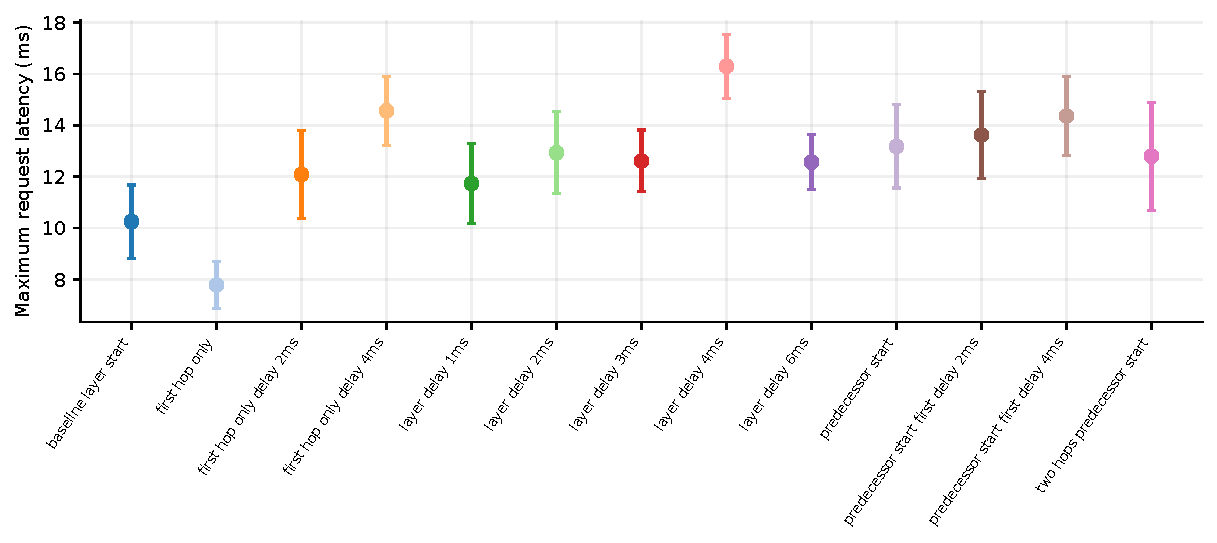
\includegraphics[width=.94\linewidth,height=.31\textheight,keepaspectratio]{figures/variants/mesh_shortest_reliable_request_latency_max_ms.pdf}\captionof{figure}{Thirteen Dynamic launch variants, M=4 and C=3; zero-delay structural rules and delay sensitivities are distinguished in the definitions.}\end{center}
\begin{center}{\scriptsize\setlength{\tabcolsep}{3pt}
\begin{tabular}{lrr}
\toprule
Variant & Mean $\pm$ SD & n \\
\midrule
baseline-layer-start & $10.250\pm1.429$ & 6 \\
first-hop-only & $7.784\pm0.911$ & 6 \\
first-hop-only-delay-2ms & $12.084\pm1.711$ & 6 \\
first-hop-only-delay-4ms & $14.567\pm1.350$ & 6 \\
layer-delay-1ms & $11.734\pm1.559$ & 6 \\
layer-delay-2ms & $12.934\pm1.592$ & 6 \\
layer-delay-3ms & $12.617\pm1.204$ & 6 \\
layer-delay-4ms & $16.300\pm1.244$ & 6 \\
layer-delay-6ms & $12.567\pm1.080$ & 6 \\
predecessor-start & $13.184\pm1.622$ & 6 \\
predecessor-start-first-delay-2ms & $13.632\pm1.705$ & 6 \\
predecessor-start-first-delay-4ms & $14.367\pm1.541$ & 6 \\
two-hops-predecessor-start & $12.800\pm2.107$ & 6 \\
\bottomrule\end{tabular}}
\captionof{table}{All thirteen variants; n counts byte-distinct trace/physics runs, not conceptual aliases.}
{\footnotesize\href{https://github.com/sanjeevkrishnaa/Compiler-Driven-ACE/blob/codex/ace-scheduler-correctness/docs/latex/qft96_final/data/variants_mesh_shortest_reliable_request_latency_max_ms.csv}{Exact CSV values and sample counts}}
\end{center}
\clearpage\subsection*{Communication makespan}
\begin{center}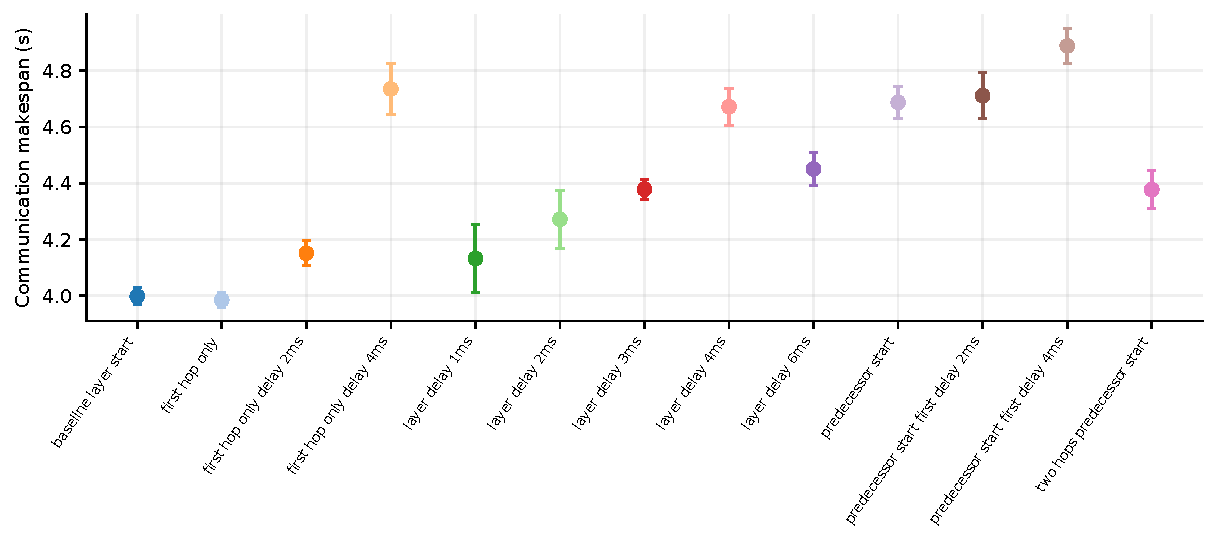
\includegraphics[width=.94\linewidth,height=.31\textheight,keepaspectratio]{figures/variants/mesh_shortest_reliable_end_to_end_latency_ms.pdf}\captionof{figure}{Thirteen Dynamic launch variants, M=4 and C=3; zero-delay structural rules and delay sensitivities are distinguished in the definitions.}\end{center}
\begin{center}{\scriptsize\setlength{\tabcolsep}{3pt}
\begin{tabular}{lrr}
\toprule
Variant & Mean $\pm$ SD & n \\
\midrule
baseline-layer-start & $3.998\pm0.031$ & 6 \\
first-hop-only & $3.985\pm0.026$ & 6 \\
first-hop-only-delay-2ms & $4.151\pm0.045$ & 6 \\
first-hop-only-delay-4ms & $4.735\pm0.091$ & 6 \\
layer-delay-1ms & $4.133\pm0.121$ & 6 \\
layer-delay-2ms & $4.272\pm0.102$ & 6 \\
layer-delay-3ms & $4.379\pm0.035$ & 6 \\
layer-delay-4ms & $4.671\pm0.067$ & 6 \\
layer-delay-6ms & $4.451\pm0.059$ & 6 \\
predecessor-start & $4.687\pm0.056$ & 6 \\
predecessor-start-first-delay-2ms & $4.711\pm0.081$ & 6 \\
predecessor-start-first-delay-4ms & $4.888\pm0.062$ & 6 \\
two-hops-predecessor-start & $4.377\pm0.066$ & 6 \\
\bottomrule\end{tabular}}
\captionof{table}{All thirteen variants; n counts byte-distinct trace/physics runs, not conceptual aliases.}
{\footnotesize\href{https://github.com/sanjeevkrishnaa/Compiler-Driven-ACE/blob/codex/ace-scheduler-correctness/docs/latex/qft96_final/data/variants_mesh_shortest_reliable_end_to_end_latency_ms.csv}{Exact CSV values and sample counts}}
\end{center}
\clearpage\subsection*{Mean admission wait}
\begin{center}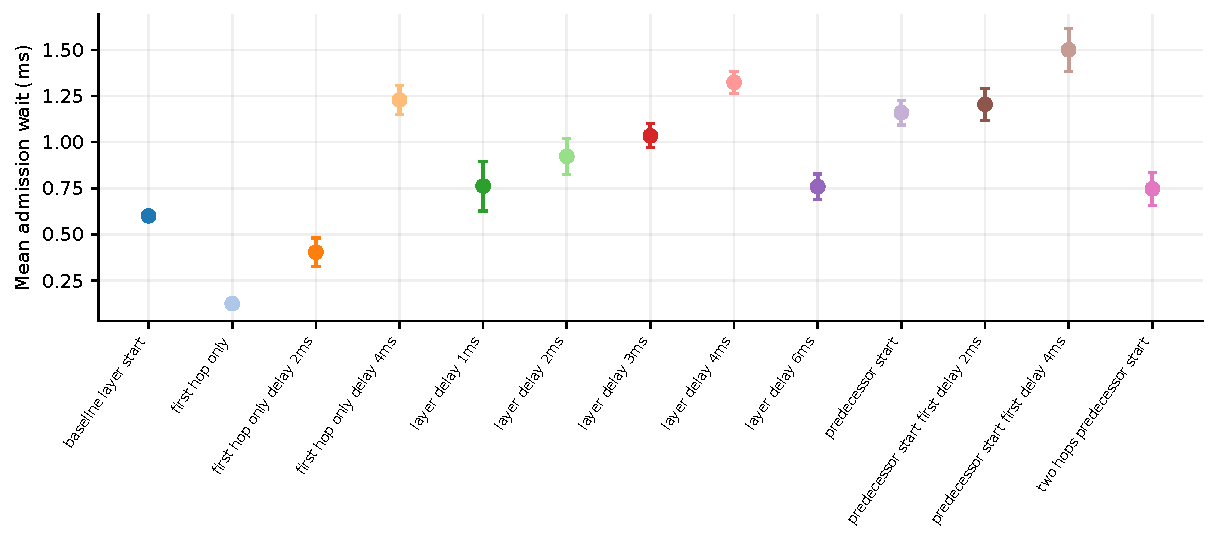
\includegraphics[width=.94\linewidth,height=.31\textheight,keepaspectratio]{figures/variants/mesh_shortest_reliable_average_admission_wait_ms.pdf}\captionof{figure}{Thirteen Dynamic launch variants, M=4 and C=3; zero-delay structural rules and delay sensitivities are distinguished in the definitions.}\end{center}
\begin{center}{\scriptsize\setlength{\tabcolsep}{3pt}
\begin{tabular}{lrr}
\toprule
Variant & Mean $\pm$ SD & n \\
\midrule
baseline-layer-start & $0.6000\pm0.0306$ & 6 \\
first-hop-only & $0.1238\pm0.0192$ & 6 \\
first-hop-only-delay-2ms & $0.4033\pm0.0767$ & 6 \\
first-hop-only-delay-4ms & $1.229\pm0.078$ & 6 \\
layer-delay-1ms & $0.7617\pm0.1353$ & 6 \\
layer-delay-2ms & $0.9227\pm0.0990$ & 6 \\
layer-delay-3ms & $1.034\pm0.065$ & 6 \\
layer-delay-4ms & $1.324\pm0.059$ & 6 \\
layer-delay-6ms & $0.7589\pm0.0685$ & 6 \\
predecessor-start & $1.160\pm0.067$ & 6 \\
predecessor-start-first-delay-2ms & $1.205\pm0.088$ & 6 \\
predecessor-start-first-delay-4ms & $1.501\pm0.116$ & 6 \\
two-hops-predecessor-start & $0.7468\pm0.0905$ & 6 \\
\bottomrule\end{tabular}}
\captionof{table}{All thirteen variants; n counts byte-distinct trace/physics runs, not conceptual aliases.}
{\footnotesize\href{https://github.com/sanjeevkrishnaa/Compiler-Driven-ACE/blob/codex/ace-scheduler-correctness/docs/latex/qft96_final/data/variants_mesh_shortest_reliable_average_admission_wait_ms.csv}{Exact CSV values and sample counts}}
\end{center}
\clearpage\subsection*{Delivered EPR fidelity}
\begin{center}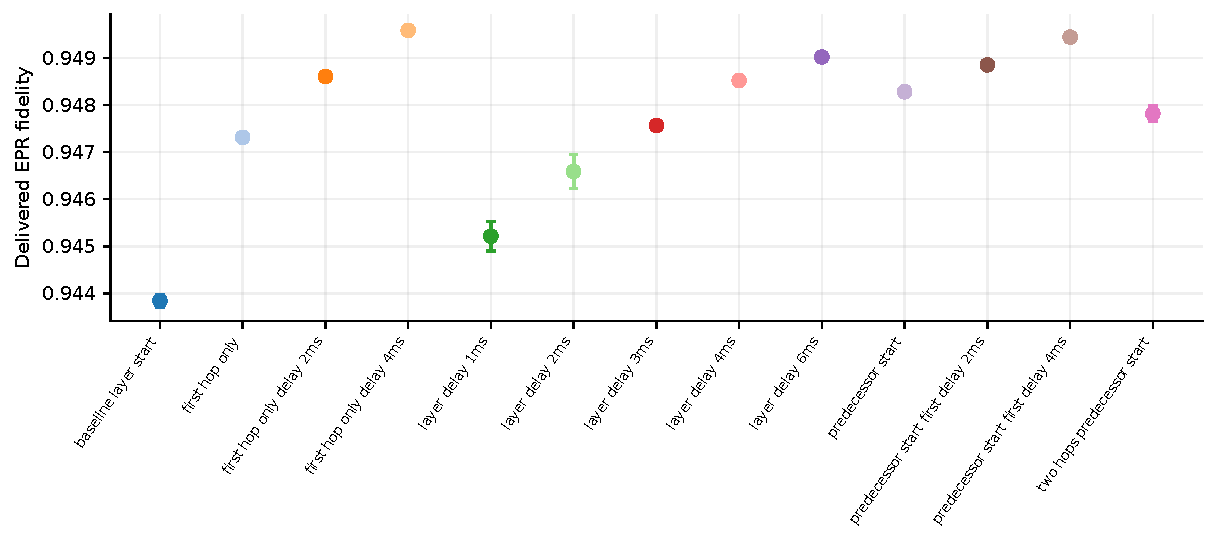
\includegraphics[width=.94\linewidth,height=.31\textheight,keepaspectratio]{figures/variants/mesh_shortest_reliable_average_delivered_epr_fidelity.pdf}\captionof{figure}{Thirteen Dynamic launch variants, M=4 and C=3; zero-delay structural rules and delay sensitivities are distinguished in the definitions.}\end{center}
\begin{center}{\scriptsize\setlength{\tabcolsep}{3pt}
\begin{tabular}{lrr}
\toprule
Variant & Mean $\pm$ SD & n \\
\midrule
baseline-layer-start & $0.9438\pm0.0001$ & 6 \\
first-hop-only & $0.9473\pm0.0001$ & 6 \\
first-hop-only-delay-2ms & $0.9486\pm0.0001$ & 6 \\
first-hop-only-delay-4ms & $0.9496\pm0.0000$ & 6 \\
layer-delay-1ms & $0.9452\pm0.0003$ & 6 \\
layer-delay-2ms & $0.9466\pm0.0004$ & 6 \\
layer-delay-3ms & $0.9476\pm0.0001$ & 6 \\
layer-delay-4ms & $0.9485\pm0.0001$ & 6 \\
layer-delay-6ms & $0.9490\pm0.0000$ & 6 \\
predecessor-start & $0.9483\pm0.0001$ & 6 \\
predecessor-start-first-delay-2ms & $0.9489\pm0.0001$ & 6 \\
predecessor-start-first-delay-4ms & $0.9494\pm0.0000$ & 6 \\
two-hops-predecessor-start & $0.9478\pm0.0002$ & 6 \\
\bottomrule\end{tabular}}
\captionof{table}{All thirteen variants; n counts byte-distinct trace/physics runs, not conceptual aliases.}
{\footnotesize\href{https://github.com/sanjeevkrishnaa/Compiler-Driven-ACE/blob/codex/ace-scheduler-correctness/docs/latex/qft96_final/data/variants_mesh_shortest_reliable_average_delivered_epr_fidelity.csv}{Exact CSV values and sample counts}}
\end{center}
\clearpage\subsection*{Compiler readiness fraction}
\begin{center}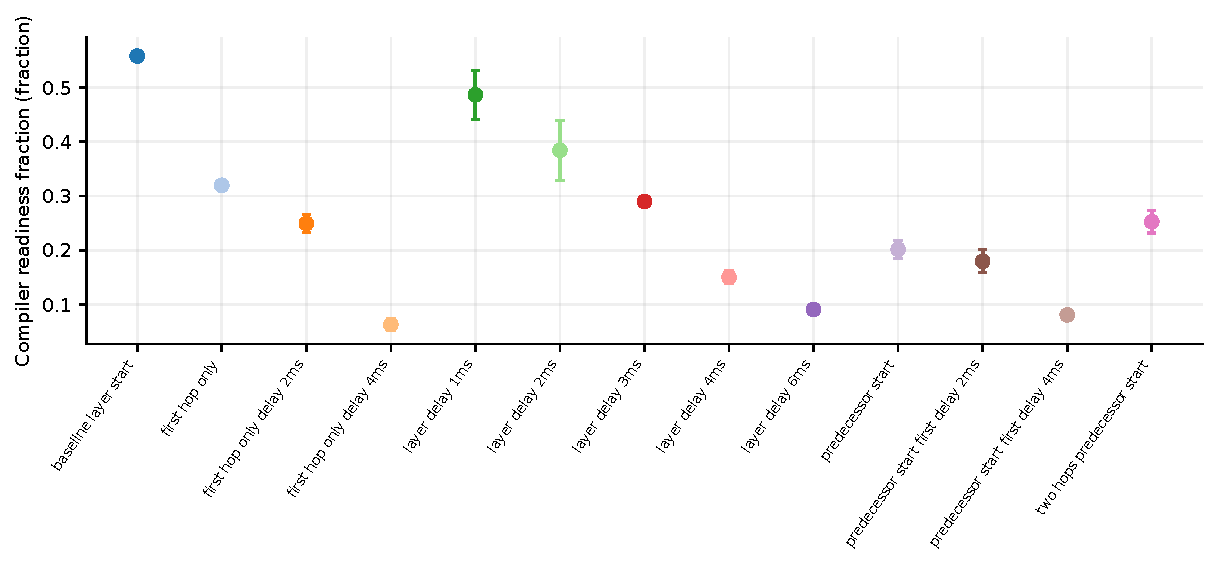
\includegraphics[width=.94\linewidth,height=.31\textheight,keepaspectratio]{figures/variants/mesh_shortest_reliable_pregenerated_success_rate.pdf}\captionof{figure}{Thirteen Dynamic launch variants, M=4 and C=3; zero-delay structural rules and delay sensitivities are distinguished in the definitions.}\end{center}
\begin{center}{\scriptsize\setlength{\tabcolsep}{3pt}
\begin{tabular}{lrr}
\toprule
Variant & Mean $\pm$ SD & n \\
\midrule
baseline-layer-start & $0.5577\pm0.0084$ & 6 \\
first-hop-only & $0.3197\pm0.0063$ & 6 \\
first-hop-only-delay-2ms & $0.2494\pm0.0166$ & 6 \\
first-hop-only-delay-4ms & $0.0632\pm0.0103$ & 6 \\
layer-delay-1ms & $0.4862\pm0.0449$ & 6 \\
layer-delay-2ms & $0.3842\pm0.0553$ & 6 \\
layer-delay-3ms & $0.2898\pm0.0070$ & 6 \\
layer-delay-4ms & $0.1504\pm0.0118$ & 6 \\
layer-delay-6ms & $0.0909\pm0.0032$ & 6 \\
predecessor-start & $0.2018\pm0.0165$ & 6 \\
predecessor-start-first-delay-2ms & $0.1797\pm0.0211$ & 6 \\
predecessor-start-first-delay-4ms & $0.0811\pm0.0091$ & 6 \\
two-hops-predecessor-start & $0.2525\pm0.0207$ & 6 \\
\bottomrule\end{tabular}}
\captionof{table}{All thirteen variants; n counts byte-distinct trace/physics runs, not conceptual aliases.}
{\footnotesize\href{https://github.com/sanjeevkrishnaa/Compiler-Driven-ACE/blob/codex/ace-scheduler-correctness/docs/latex/qft96_final/data/variants_mesh_shortest_reliable_pregenerated_success_rate.csv}{Exact CSV values and sample counts}}
\end{center}
\clearpage\subsection*{Intended compiler-hit fraction}
\begin{center}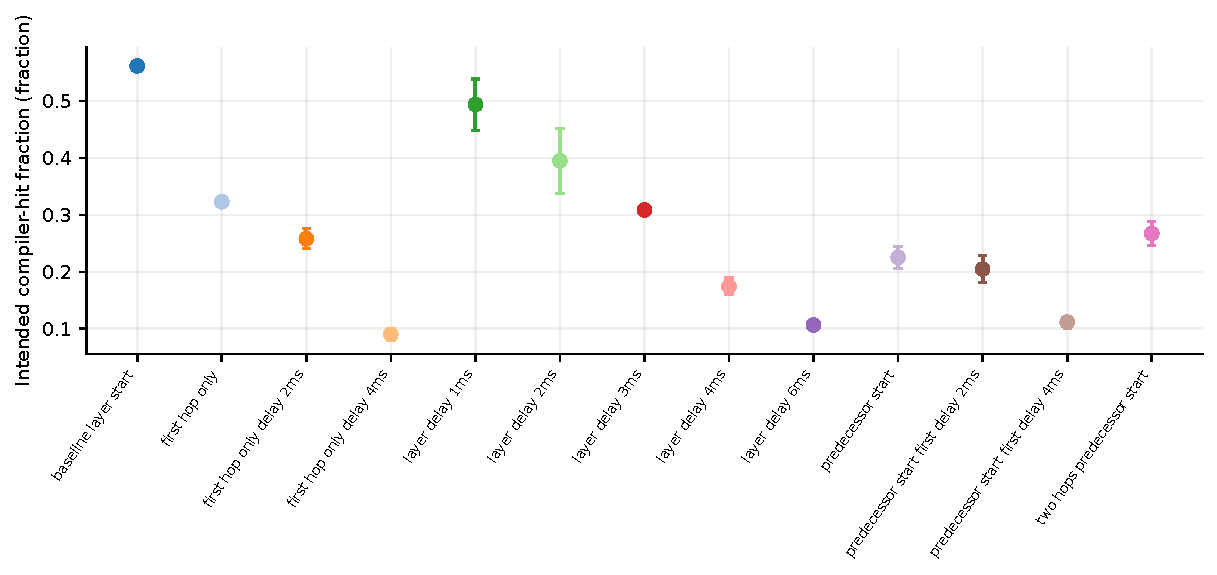
\includegraphics[width=.94\linewidth,height=.31\textheight,keepaspectratio]{figures/variants/mesh_shortest_reliable_intended_request_hit_rate.pdf}\captionof{figure}{Thirteen Dynamic launch variants, M=4 and C=3; zero-delay structural rules and delay sensitivities are distinguished in the definitions.}\end{center}
\begin{center}{\scriptsize\setlength{\tabcolsep}{3pt}
\begin{tabular}{lrr}
\toprule
Variant & Mean $\pm$ SD & n \\
\midrule
baseline-layer-start & $0.5618\pm0.0079$ & 6 \\
first-hop-only & $0.3231\pm0.0055$ & 6 \\
first-hop-only-delay-2ms & $0.2585\pm0.0171$ & 6 \\
first-hop-only-delay-4ms & $0.0902\pm0.0102$ & 6 \\
layer-delay-1ms & $0.4940\pm0.0449$ & 6 \\
layer-delay-2ms & $0.3950\pm0.0569$ & 6 \\
layer-delay-3ms & $0.3088\pm0.0073$ & 6 \\
layer-delay-4ms & $0.1746\pm0.0147$ & 6 \\
layer-delay-6ms & $0.1068\pm0.0034$ & 6 \\
predecessor-start & $0.2255\pm0.0189$ & 6 \\
predecessor-start-first-delay-2ms & $0.2049\pm0.0237$ & 6 \\
predecessor-start-first-delay-4ms & $0.1119\pm0.0105$ & 6 \\
two-hops-predecessor-start & $0.2674\pm0.0209$ & 6 \\
\bottomrule\end{tabular}}
\captionof{table}{All thirteen variants; n counts byte-distinct trace/physics runs, not conceptual aliases.}
{\footnotesize\href{https://github.com/sanjeevkrishnaa/Compiler-Driven-ACE/blob/codex/ace-scheduler-correctness/docs/latex/qft96_final/data/variants_mesh_shortest_reliable_intended_request_hit_rate.csv}{Exact CSV values and sample counts}}
\end{center}
\clearpage\subsection*{Compiler fallback fraction}
\begin{center}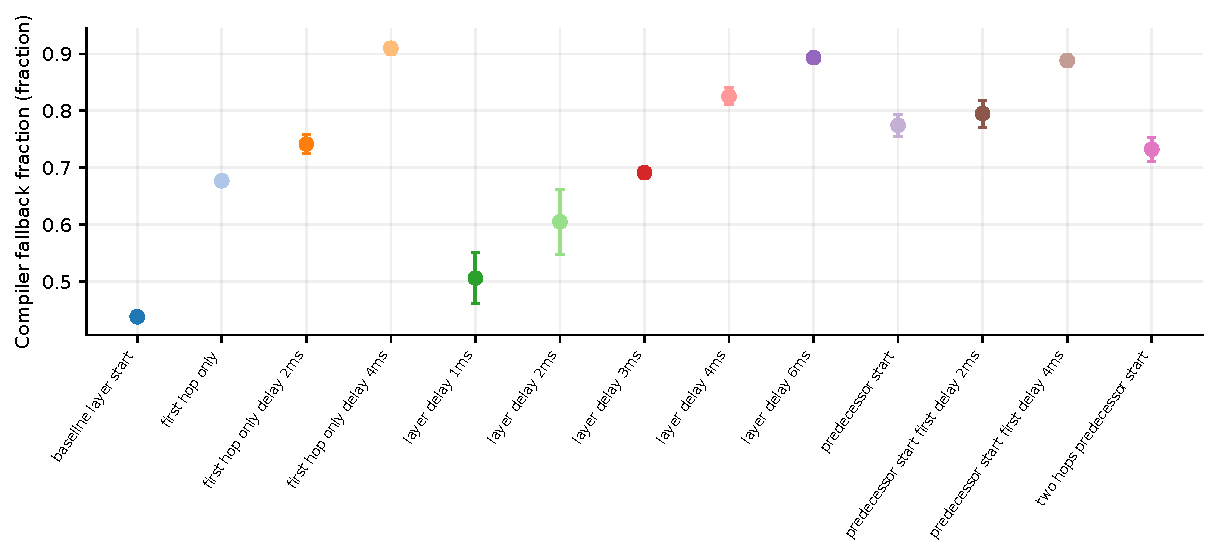
\includegraphics[width=.94\linewidth,height=.31\textheight,keepaspectratio]{figures/variants/mesh_shortest_reliable_on_demand_fallback_rate.pdf}\captionof{figure}{Thirteen Dynamic launch variants, M=4 and C=3; zero-delay structural rules and delay sensitivities are distinguished in the definitions.}\end{center}
\begin{center}{\scriptsize\setlength{\tabcolsep}{3pt}
\begin{tabular}{lrr}
\toprule
Variant & Mean $\pm$ SD & n \\
\midrule
baseline-layer-start & $0.4382\pm0.0079$ & 6 \\
first-hop-only & $0.6769\pm0.0055$ & 6 \\
first-hop-only-delay-2ms & $0.7415\pm0.0171$ & 6 \\
first-hop-only-delay-4ms & $0.9098\pm0.0102$ & 6 \\
layer-delay-1ms & $0.5060\pm0.0449$ & 6 \\
layer-delay-2ms & $0.6050\pm0.0569$ & 6 \\
layer-delay-3ms & $0.6912\pm0.0073$ & 6 \\
layer-delay-4ms & $0.8254\pm0.0147$ & 6 \\
layer-delay-6ms & $0.8932\pm0.0034$ & 6 \\
predecessor-start & $0.7745\pm0.0189$ & 6 \\
predecessor-start-first-delay-2ms & $0.7951\pm0.0237$ & 6 \\
predecessor-start-first-delay-4ms & $0.8881\pm0.0105$ & 6 \\
two-hops-predecessor-start & $0.7326\pm0.0209$ & 6 \\
\bottomrule\end{tabular}}
\captionof{table}{All thirteen variants; n counts byte-distinct trace/physics runs, not conceptual aliases.}
{\footnotesize\href{https://github.com/sanjeevkrishnaa/Compiler-Driven-ACE/blob/codex/ace-scheduler-correctness/docs/latex/qft96_final/data/variants_mesh_shortest_reliable_on_demand_fallback_rate.csv}{Exact CSV values and sample counts}}
\end{center}
\clearpage\subsection*{Compiler-cache waste}
\begin{center}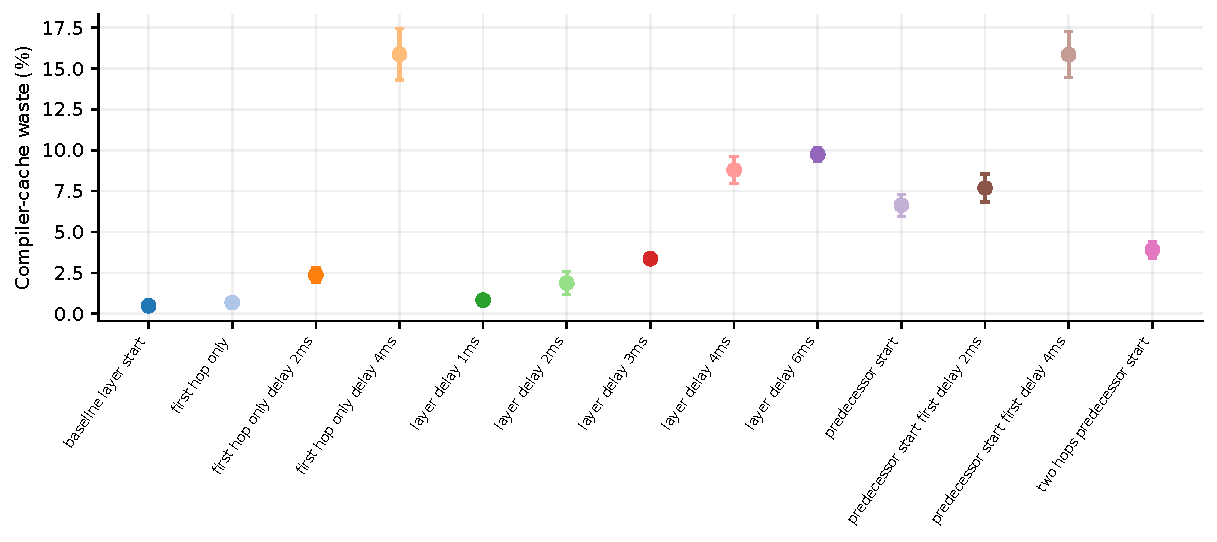
\includegraphics[width=.94\linewidth,height=.31\textheight,keepaspectratio]{figures/variants/mesh_shortest_reliable_compiler_waste_percentage.pdf}\captionof{figure}{Thirteen Dynamic launch variants, M=4 and C=3; zero-delay structural rules and delay sensitivities are distinguished in the definitions.}\end{center}
\begin{center}{\scriptsize\setlength{\tabcolsep}{3pt}
\begin{tabular}{lrr}
\toprule
Variant & Mean $\pm$ SD & n \\
\midrule
baseline-layer-start & $0.4870\pm0.0873$ & 6 \\
first-hop-only & $0.6862\pm0.1865$ & 6 \\
first-hop-only-delay-2ms & $2.361\pm0.471$ & 6 \\
first-hop-only-delay-4ms & $15.870\pm1.577$ & 6 \\
layer-delay-1ms & $0.8349\pm0.2362$ & 6 \\
layer-delay-2ms & $1.876\pm0.725$ & 6 \\
layer-delay-3ms & $3.366\pm0.199$ & 6 \\
layer-delay-4ms & $8.791\pm0.804$ & 6 \\
layer-delay-6ms & $9.742\pm0.427$ & 6 \\
predecessor-start & $6.639\pm0.667$ & 6 \\
predecessor-start-first-delay-2ms & $7.690\pm0.855$ & 6 \\
predecessor-start-first-delay-4ms & $15.846\pm1.412$ & 6 \\
two-hops-predecessor-start & $3.907\pm0.525$ & 6 \\
\bottomrule\end{tabular}}
\captionof{table}{All thirteen variants; n counts byte-distinct trace/physics runs, not conceptual aliases.}
{\footnotesize\href{https://github.com/sanjeevkrishnaa/Compiler-Driven-ACE/blob/codex/ace-scheduler-correctness/docs/latex/qft96_final/data/variants_mesh_shortest_reliable_compiler_waste_percentage.csv}{Exact CSV values and sample counts}}
\end{center}
\clearpage\subsection*{Native-protocol waste}
\begin{center}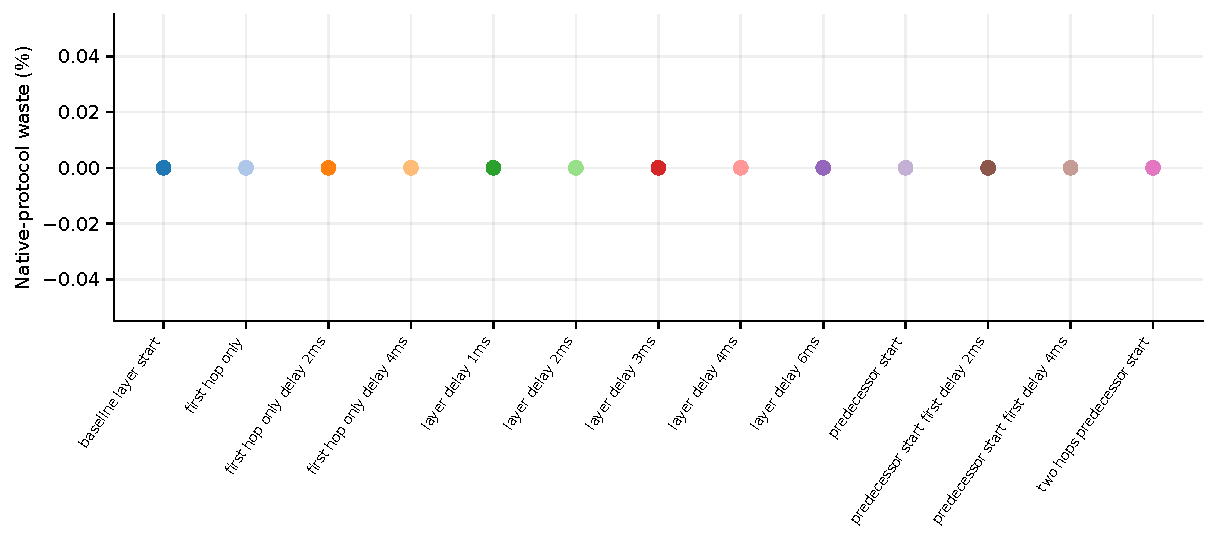
\includegraphics[width=.94\linewidth,height=.31\textheight,keepaspectratio]{figures/variants/mesh_shortest_reliable_protocol_waste_percentage.pdf}\captionof{figure}{Thirteen Dynamic launch variants, M=4 and C=3; zero-delay structural rules and delay sensitivities are distinguished in the definitions.}\end{center}
\begin{center}{\scriptsize\setlength{\tabcolsep}{3pt}
\begin{tabular}{lrr}
\toprule
Variant & Mean $\pm$ SD & n \\
\midrule
baseline-layer-start & $0.0000\pm0.0000$ & 6 \\
first-hop-only & $0.0000\pm0.0000$ & 6 \\
first-hop-only-delay-2ms & $0.0000\pm0.0000$ & 6 \\
first-hop-only-delay-4ms & $0.0000\pm0.0000$ & 6 \\
layer-delay-1ms & $0.0000\pm0.0000$ & 6 \\
layer-delay-2ms & $0.0000\pm0.0000$ & 6 \\
layer-delay-3ms & $0.0000\pm0.0000$ & 6 \\
layer-delay-4ms & $0.0000\pm0.0000$ & 6 \\
layer-delay-6ms & $0.0000\pm0.0000$ & 6 \\
predecessor-start & $0.0000\pm0.0000$ & 6 \\
predecessor-start-first-delay-2ms & $0.0000\pm0.0000$ & 6 \\
predecessor-start-first-delay-4ms & $0.0000\pm0.0000$ & 6 \\
two-hops-predecessor-start & $0.0000\pm0.0000$ & 6 \\
\bottomrule\end{tabular}}
\captionof{table}{All thirteen variants; n counts byte-distinct trace/physics runs, not conceptual aliases.}
{\footnotesize\href{https://github.com/sanjeevkrishnaa/Compiler-Driven-ACE/blob/codex/ace-scheduler-correctness/docs/latex/qft96_final/data/variants_mesh_shortest_reliable_protocol_waste_percentage.csv}{Exact CSV values and sample counts}}
\end{center}
\clearpage\subsection*{Compiler-pair expiry}
\begin{center}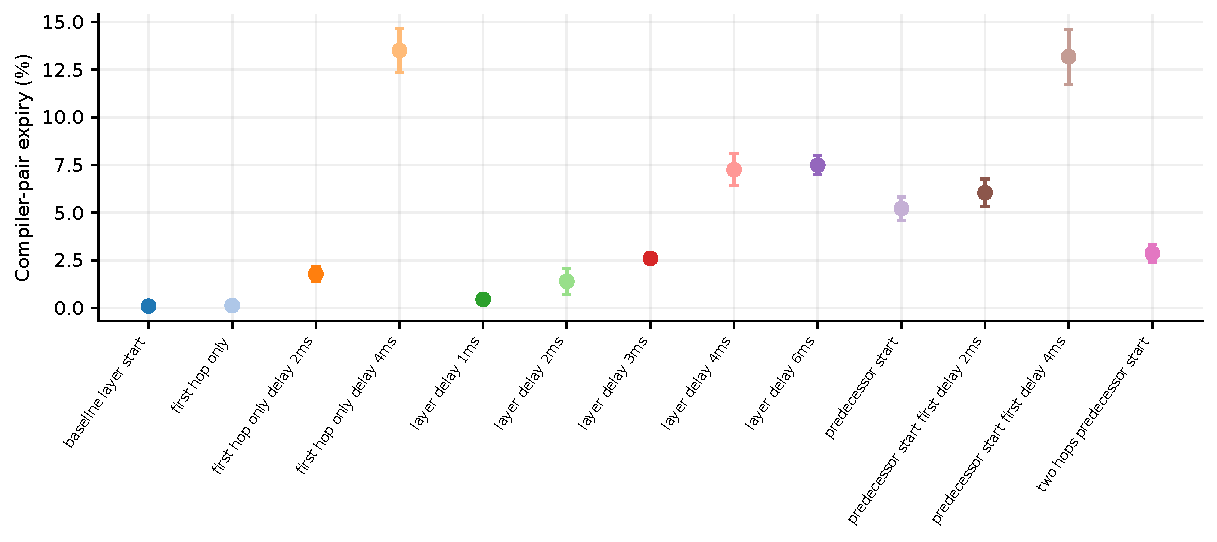
\includegraphics[width=.94\linewidth,height=.31\textheight,keepaspectratio]{figures/variants/mesh_shortest_reliable_compiler_expiry_percentage.pdf}\captionof{figure}{Thirteen Dynamic launch variants, M=4 and C=3; zero-delay structural rules and delay sensitivities are distinguished in the definitions.}\end{center}
\begin{center}{\scriptsize\setlength{\tabcolsep}{3pt}
\begin{tabular}{lrr}
\toprule
Variant & Mean $\pm$ SD & n \\
\midrule
baseline-layer-start & $0.0916\pm0.0585$ & 6 \\
first-hop-only & $0.1184\pm0.0822$ & 6 \\
first-hop-only-delay-2ms & $1.774\pm0.395$ & 6 \\
first-hop-only-delay-4ms & $13.507\pm1.153$ & 6 \\
layer-delay-1ms & $0.4481\pm0.2454$ & 6 \\
layer-delay-2ms & $1.391\pm0.696$ & 6 \\
layer-delay-3ms & $2.599\pm0.182$ & 6 \\
layer-delay-4ms & $7.242\pm0.841$ & 6 \\
layer-delay-6ms & $7.484\pm0.507$ & 6 \\
predecessor-start & $5.213\pm0.605$ & 6 \\
predecessor-start-first-delay-2ms & $6.036\pm0.725$ & 6 \\
predecessor-start-first-delay-4ms & $13.182\pm1.440$ & 6 \\
two-hops-predecessor-start & $2.867\pm0.462$ & 6 \\
\bottomrule\end{tabular}}
\captionof{table}{All thirteen variants; n counts byte-distinct trace/physics runs, not conceptual aliases.}
{\footnotesize\href{https://github.com/sanjeevkrishnaa/Compiler-Driven-ACE/blob/codex/ace-scheduler-correctness/docs/latex/qft96_final/data/variants_mesh_shortest_reliable_compiler_expiry_percentage.csv}{Exact CSV values and sample counts}}
\end{center}
\clearpage\subsection*{Used compiler-pair storage time}
\begin{center}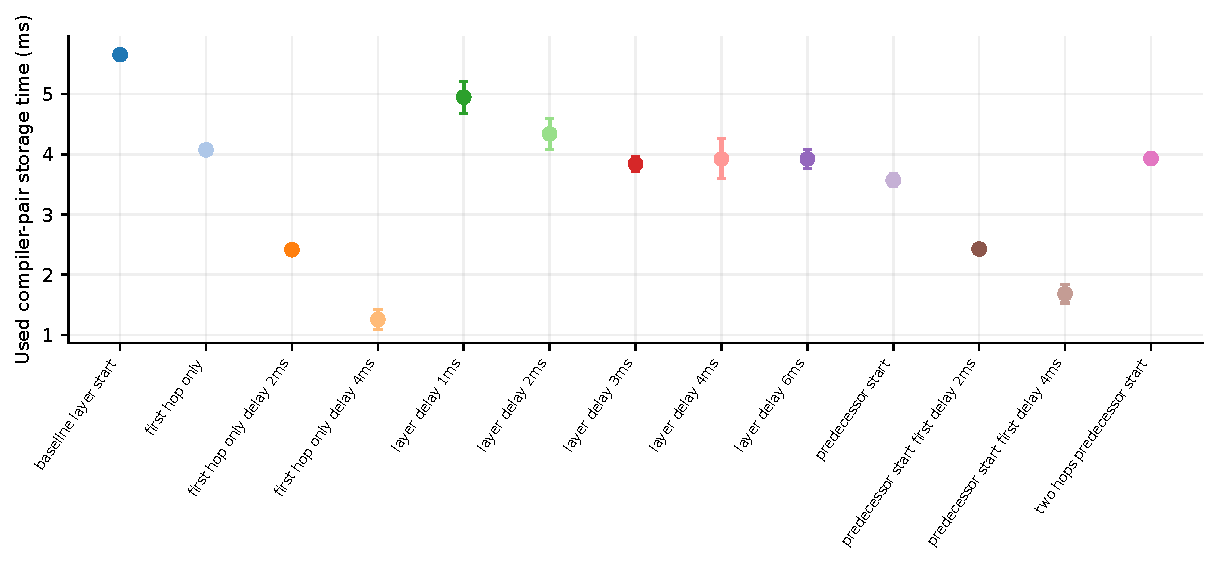
\includegraphics[width=.94\linewidth,height=.31\textheight,keepaspectratio]{figures/variants/mesh_shortest_reliable_average_storage_time_ms.pdf}\captionof{figure}{Thirteen Dynamic launch variants, M=4 and C=3; zero-delay structural rules and delay sensitivities are distinguished in the definitions.}\end{center}
\begin{center}{\scriptsize\setlength{\tabcolsep}{3pt}
\begin{tabular}{lrr}
\toprule
Variant & Mean $\pm$ SD & n \\
\midrule
baseline-layer-start & $5.649\pm0.071$ & 6 \\
first-hop-only & $4.070\pm0.019$ & 6 \\
first-hop-only-delay-2ms & $2.416\pm0.053$ & 6 \\
first-hop-only-delay-4ms & $1.260\pm0.161$ & 6 \\
layer-delay-1ms & $4.946\pm0.266$ & 6 \\
layer-delay-2ms & $4.336\pm0.257$ & 6 \\
layer-delay-3ms & $3.839\pm0.130$ & 6 \\
layer-delay-4ms & $3.922\pm0.333$ & 6 \\
layer-delay-6ms & $3.922\pm0.155$ & 6 \\
predecessor-start & $3.567\pm0.107$ & 6 \\
predecessor-start-first-delay-2ms & $2.427\pm0.071$ & 6 \\
predecessor-start-first-delay-4ms & $1.685\pm0.152$ & 6 \\
two-hops-predecessor-start & $3.927\pm0.046$ & 6 \\
\bottomrule\end{tabular}}
\captionof{table}{All thirteen variants; n counts byte-distinct trace/physics runs, not conceptual aliases.}
{\footnotesize\href{https://github.com/sanjeevkrishnaa/Compiler-Driven-ACE/blob/codex/ace-scheduler-correctness/docs/latex/qft96_final/data/variants_mesh_shortest_reliable_average_storage_time_ms.csv}{Exact CSV values and sample counts}}
\end{center}
\clearpage\subsection*{Delivered-hop throughput}
\begin{center}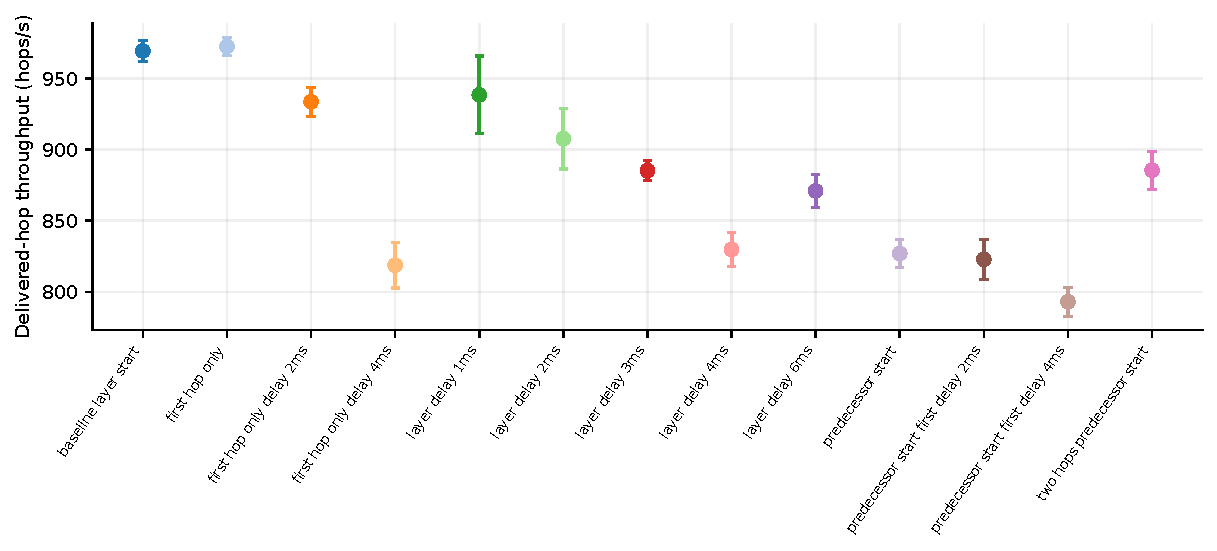
\includegraphics[width=.94\linewidth,height=.31\textheight,keepaspectratio]{figures/variants/mesh_shortest_reliable_hop_throughput_s.pdf}\captionof{figure}{Thirteen Dynamic launch variants, M=4 and C=3; zero-delay structural rules and delay sensitivities are distinguished in the definitions.}\end{center}
\begin{center}{\scriptsize\setlength{\tabcolsep}{3pt}
\begin{tabular}{lrr}
\toprule
Variant & Mean $\pm$ SD & n \\
\midrule
baseline-layer-start & $969.43\pm7.48$ & 6 \\
first-hop-only & $972.64\pm6.28$ & 6 \\
first-hop-only-delay-2ms & $933.73\pm10.12$ & 6 \\
first-hop-only-delay-4ms & $818.84\pm16.10$ & 6 \\
layer-delay-1ms & $938.56\pm27.34$ & 6 \\
layer-delay-2ms & $907.74\pm21.31$ & 6 \\
layer-delay-3ms & $885.23\pm7.18$ & 6 \\
layer-delay-4ms & $829.86\pm11.98$ & 6 \\
layer-delay-6ms & $871.00\pm11.70$ & 6 \\
predecessor-start & $827.02\pm9.90$ & 6 \\
predecessor-start-first-delay-2ms & $822.88\pm14.09$ & 6 \\
predecessor-start-first-delay-4ms & $793.04\pm10.13$ & 6 \\
two-hops-predecessor-start & $885.63\pm13.36$ & 6 \\
\bottomrule\end{tabular}}
\captionof{table}{All thirteen variants; n counts byte-distinct trace/physics runs, not conceptual aliases.}
{\footnotesize\href{https://github.com/sanjeevkrishnaa/Compiler-Driven-ACE/blob/codex/ace-scheduler-correctness/docs/latex/qft96_final/data/variants_mesh_shortest_reliable_hop_throughput_s.csv}{Exact CSV values and sample counts}}
\end{center}
\clearpage\subsection*{Completion fraction}
\begin{center}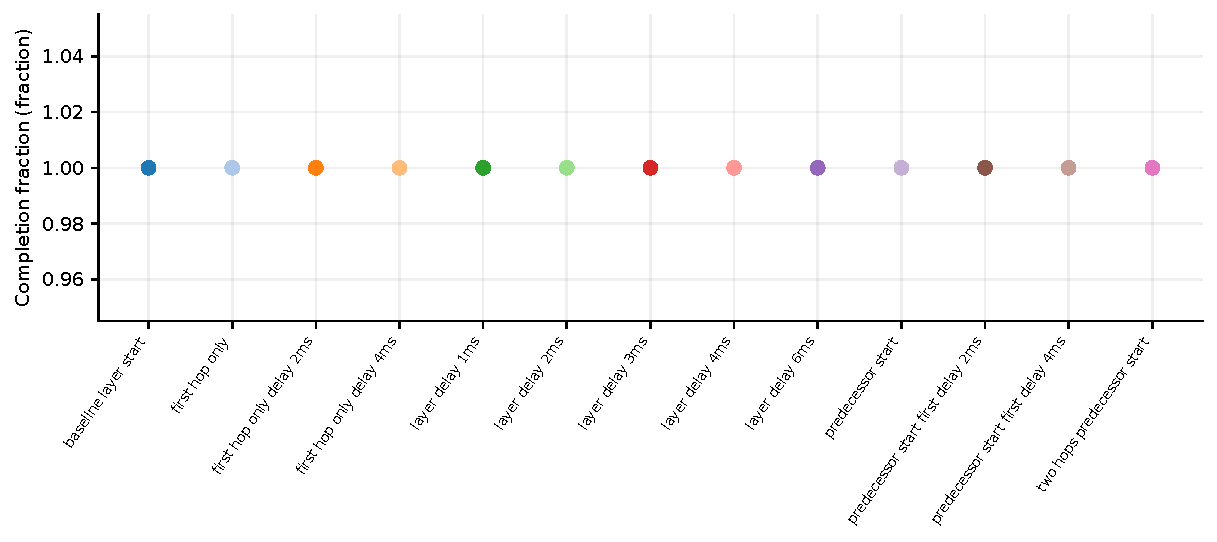
\includegraphics[width=.94\linewidth,height=.31\textheight,keepaspectratio]{figures/variants/mesh_shortest_reliable_completion_rate.pdf}\captionof{figure}{Thirteen Dynamic launch variants, M=4 and C=3; zero-delay structural rules and delay sensitivities are distinguished in the definitions.}\end{center}
\begin{center}{\scriptsize\setlength{\tabcolsep}{3pt}
\begin{tabular}{lrr}
\toprule
Variant & Mean $\pm$ SD & n \\
\midrule
baseline-layer-start & $1.000\pm0.000$ & 6 \\
first-hop-only & $1.000\pm0.000$ & 6 \\
first-hop-only-delay-2ms & $1.000\pm0.000$ & 6 \\
first-hop-only-delay-4ms & $1.000\pm0.000$ & 6 \\
layer-delay-1ms & $1.000\pm0.000$ & 6 \\
layer-delay-2ms & $1.000\pm0.000$ & 6 \\
layer-delay-3ms & $1.000\pm0.000$ & 6 \\
layer-delay-4ms & $1.000\pm0.000$ & 6 \\
layer-delay-6ms & $1.000\pm0.000$ & 6 \\
predecessor-start & $1.000\pm0.000$ & 6 \\
predecessor-start-first-delay-2ms & $1.000\pm0.000$ & 6 \\
predecessor-start-first-delay-4ms & $1.000\pm0.000$ & 6 \\
two-hops-predecessor-start & $1.000\pm0.000$ & 6 \\
\bottomrule\end{tabular}}
\captionof{table}{All thirteen variants; n counts byte-distinct trace/physics runs, not conceptual aliases.}
{\footnotesize\href{https://github.com/sanjeevkrishnaa/Compiler-Driven-ACE/blob/codex/ace-scheduler-correctness/docs/latex/qft96_final/data/variants_mesh_shortest_reliable_completion_rate.csv}{Exact CSV values and sample counts}}
\end{center}
\section{Mesh / max\_reliability}
\clearpage\subsection*{Mean request latency}
\begin{center}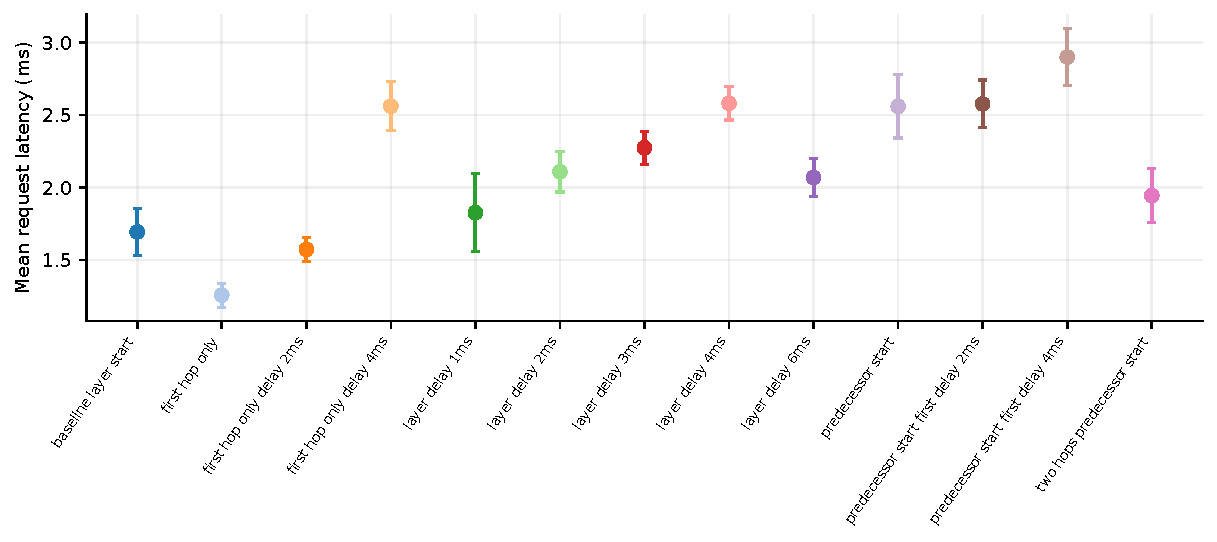
\includegraphics[width=.94\linewidth,height=.31\textheight,keepaspectratio]{figures/variants/mesh_max_reliability_request_latency_mean_ms.pdf}\captionof{figure}{Thirteen Dynamic launch variants, M=4 and C=3; zero-delay structural rules and delay sensitivities are distinguished in the definitions.}\end{center}
\begin{center}{\scriptsize\setlength{\tabcolsep}{3pt}
\begin{tabular}{lrr}
\toprule
Variant & Mean $\pm$ SD & n \\
\midrule
baseline-layer-start & $1.693\pm0.164$ & 6 \\
first-hop-only & $1.257\pm0.083$ & 6 \\
first-hop-only-delay-2ms & $1.573\pm0.080$ & 6 \\
first-hop-only-delay-4ms & $2.561\pm0.170$ & 6 \\
layer-delay-1ms & $1.826\pm0.270$ & 6 \\
layer-delay-2ms & $2.108\pm0.139$ & 6 \\
layer-delay-3ms & $2.274\pm0.114$ & 6 \\
layer-delay-4ms & $2.582\pm0.116$ & 6 \\
layer-delay-6ms & $2.070\pm0.131$ & 6 \\
predecessor-start & $2.560\pm0.218$ & 6 \\
predecessor-start-first-delay-2ms & $2.577\pm0.165$ & 6 \\
predecessor-start-first-delay-4ms & $2.900\pm0.198$ & 6 \\
two-hops-predecessor-start & $1.945\pm0.189$ & 6 \\
\bottomrule\end{tabular}}
\captionof{table}{All thirteen variants; n counts byte-distinct trace/physics runs, not conceptual aliases.}
{\footnotesize\href{https://github.com/sanjeevkrishnaa/Compiler-Driven-ACE/blob/codex/ace-scheduler-correctness/docs/latex/qft96_final/data/variants_mesh_max_reliability_request_latency_mean_ms.csv}{Exact CSV values and sample counts}}
\end{center}
\clearpage\subsection*{Median request latency}
\begin{center}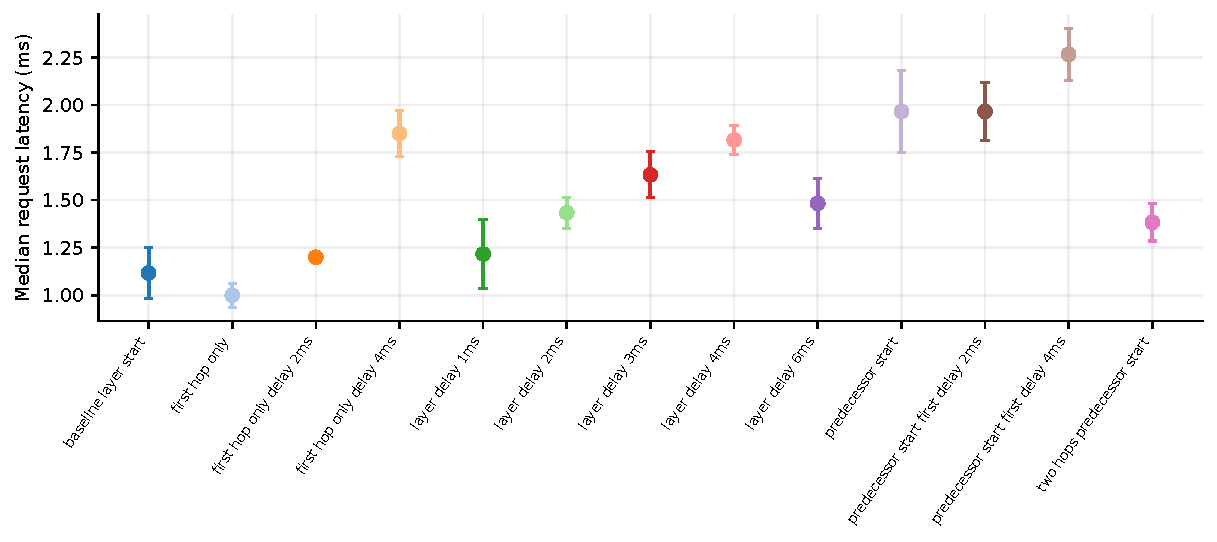
\includegraphics[width=.94\linewidth,height=.31\textheight,keepaspectratio]{figures/variants/mesh_max_reliability_request_latency_median_ms.pdf}\captionof{figure}{Thirteen Dynamic launch variants, M=4 and C=3; zero-delay structural rules and delay sensitivities are distinguished in the definitions.}\end{center}
\begin{center}{\scriptsize\setlength{\tabcolsep}{3pt}
\begin{tabular}{lrr}
\toprule
Variant & Mean $\pm$ SD & n \\
\midrule
baseline-layer-start & $1.117\pm0.133$ & 6 \\
first-hop-only & $1.000\pm0.063$ & 6 \\
first-hop-only-delay-2ms & $1.200\pm0.000$ & 6 \\
first-hop-only-delay-4ms & $1.850\pm0.122$ & 6 \\
layer-delay-1ms & $1.217\pm0.183$ & 6 \\
layer-delay-2ms & $1.433\pm0.082$ & 6 \\
layer-delay-3ms & $1.633\pm0.121$ & 6 \\
layer-delay-4ms & $1.817\pm0.075$ & 6 \\
layer-delay-6ms & $1.483\pm0.133$ & 6 \\
predecessor-start & $1.967\pm0.216$ & 6 \\
predecessor-start-first-delay-2ms & $1.967\pm0.151$ & 6 \\
predecessor-start-first-delay-4ms & $2.267\pm0.137$ & 6 \\
two-hops-predecessor-start & $1.383\pm0.098$ & 6 \\
\bottomrule\end{tabular}}
\captionof{table}{All thirteen variants; n counts byte-distinct trace/physics runs, not conceptual aliases.}
{\footnotesize\href{https://github.com/sanjeevkrishnaa/Compiler-Driven-ACE/blob/codex/ace-scheduler-correctness/docs/latex/qft96_final/data/variants_mesh_max_reliability_request_latency_median_ms.csv}{Exact CSV values and sample counts}}
\end{center}
\clearpage\subsection*{p95 request latency}
\begin{center}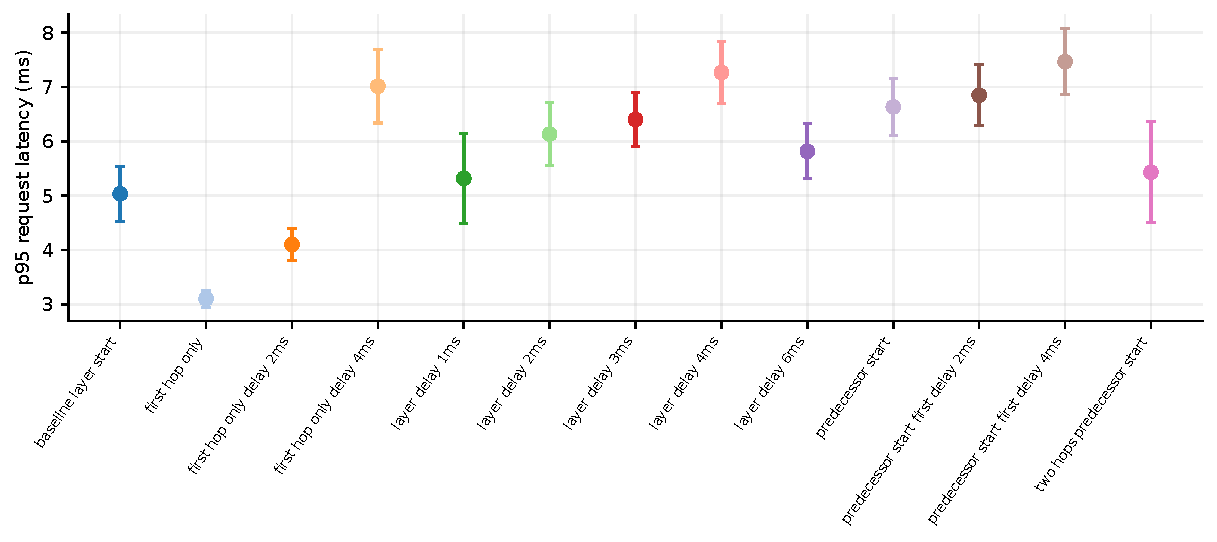
\includegraphics[width=.94\linewidth,height=.31\textheight,keepaspectratio]{figures/variants/mesh_max_reliability_request_latency_p95_ms.pdf}\captionof{figure}{Thirteen Dynamic launch variants, M=4 and C=3; zero-delay structural rules and delay sensitivities are distinguished in the definitions.}\end{center}
\begin{center}{\scriptsize\setlength{\tabcolsep}{3pt}
\begin{tabular}{lrr}
\toprule
Variant & Mean $\pm$ SD & n \\
\midrule
baseline-layer-start & $5.033\pm0.509$ & 6 \\
first-hop-only & $3.100\pm0.155$ & 6 \\
first-hop-only-delay-2ms & $4.100\pm0.297$ & 6 \\
first-hop-only-delay-4ms & $7.017\pm0.679$ & 6 \\
layer-delay-1ms & $5.317\pm0.823$ & 6 \\
layer-delay-2ms & $6.133\pm0.575$ & 6 \\
layer-delay-3ms & $6.400\pm0.498$ & 6 \\
layer-delay-4ms & $7.265\pm0.567$ & 6 \\
layer-delay-6ms & $5.817\pm0.504$ & 6 \\
predecessor-start & $6.633\pm0.524$ & 6 \\
predecessor-start-first-delay-2ms & $6.850\pm0.561$ & 6 \\
predecessor-start-first-delay-4ms & $7.467\pm0.612$ & 6 \\
two-hops-predecessor-start & $5.433\pm0.933$ & 6 \\
\bottomrule\end{tabular}}
\captionof{table}{All thirteen variants; n counts byte-distinct trace/physics runs, not conceptual aliases.}
{\footnotesize\href{https://github.com/sanjeevkrishnaa/Compiler-Driven-ACE/blob/codex/ace-scheduler-correctness/docs/latex/qft96_final/data/variants_mesh_max_reliability_request_latency_p95_ms.csv}{Exact CSV values and sample counts}}
\end{center}
\clearpage\subsection*{Maximum request latency}
\begin{center}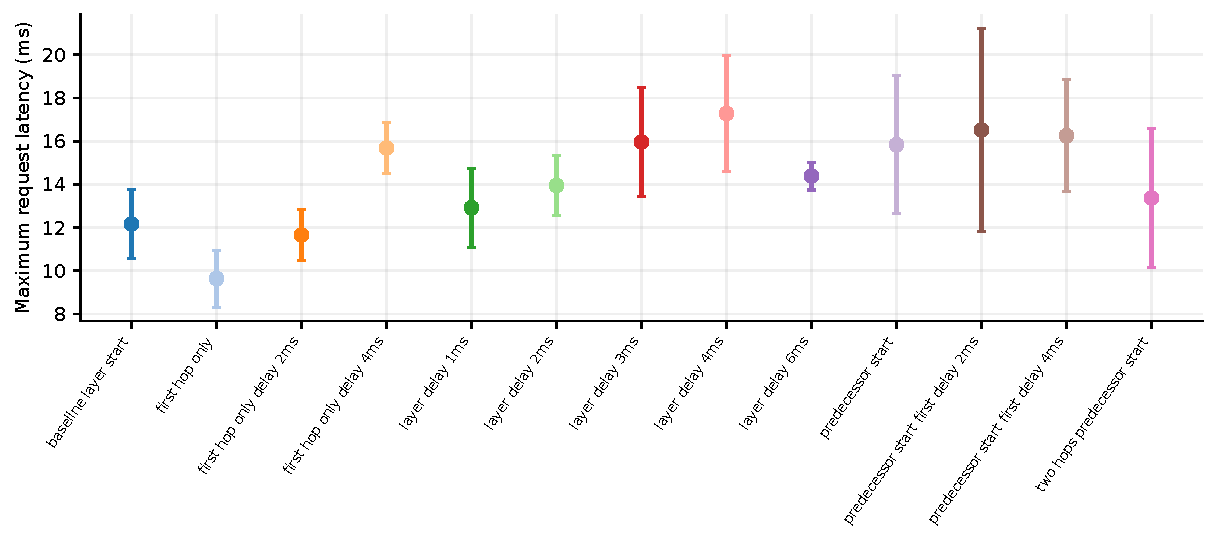
\includegraphics[width=.94\linewidth,height=.31\textheight,keepaspectratio]{figures/variants/mesh_max_reliability_request_latency_max_ms.pdf}\captionof{figure}{Thirteen Dynamic launch variants, M=4 and C=3; zero-delay structural rules and delay sensitivities are distinguished in the definitions.}\end{center}
\begin{center}{\scriptsize\setlength{\tabcolsep}{3pt}
\begin{tabular}{lrr}
\toprule
Variant & Mean $\pm$ SD & n \\
\midrule
baseline-layer-start & $12.167\pm1.598$ & 6 \\
first-hop-only & $9.634\pm1.322$ & 6 \\
first-hop-only-delay-2ms & $11.650\pm1.185$ & 6 \\
first-hop-only-delay-4ms & $15.684\pm1.184$ & 6 \\
layer-delay-1ms & $12.917\pm1.819$ & 6 \\
layer-delay-2ms & $13.950\pm1.397$ & 6 \\
layer-delay-3ms & $15.967\pm2.518$ & 6 \\
layer-delay-4ms & $17.284\pm2.678$ & 6 \\
layer-delay-6ms & $14.384\pm0.643$ & 6 \\
predecessor-start & $15.834\pm3.190$ & 6 \\
predecessor-start-first-delay-2ms & $16.517\pm4.703$ & 6 \\
predecessor-start-first-delay-4ms & $16.250\pm2.589$ & 6 \\
two-hops-predecessor-start & $13.365\pm3.232$ & 6 \\
\bottomrule\end{tabular}}
\captionof{table}{All thirteen variants; n counts byte-distinct trace/physics runs, not conceptual aliases.}
{\footnotesize\href{https://github.com/sanjeevkrishnaa/Compiler-Driven-ACE/blob/codex/ace-scheduler-correctness/docs/latex/qft96_final/data/variants_mesh_max_reliability_request_latency_max_ms.csv}{Exact CSV values and sample counts}}
\end{center}
\clearpage\subsection*{Communication makespan}
\begin{center}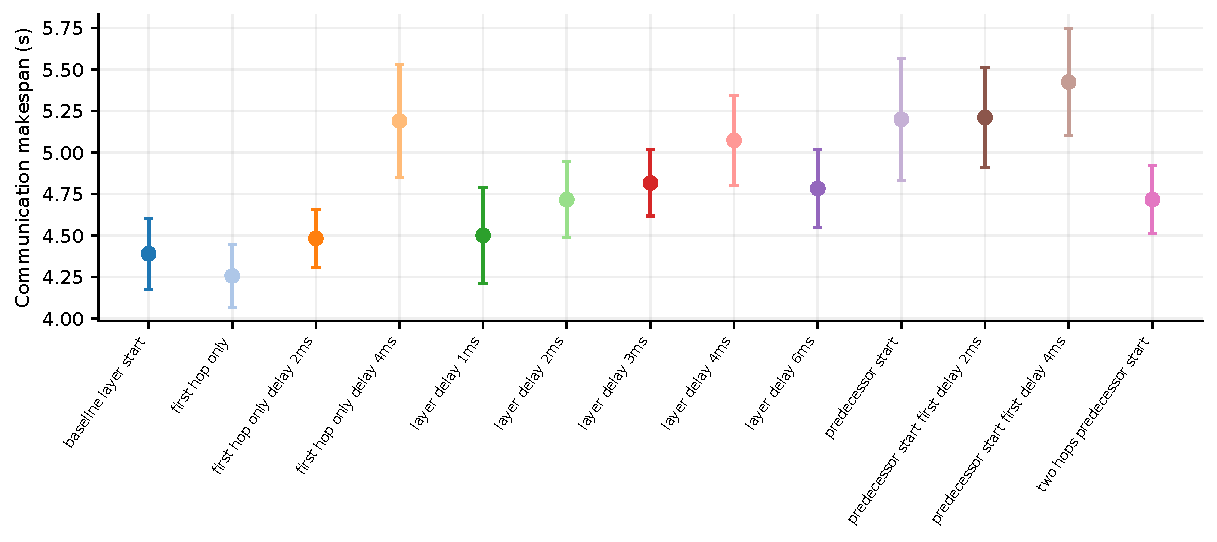
\includegraphics[width=.94\linewidth,height=.31\textheight,keepaspectratio]{figures/variants/mesh_max_reliability_end_to_end_latency_ms.pdf}\captionof{figure}{Thirteen Dynamic launch variants, M=4 and C=3; zero-delay structural rules and delay sensitivities are distinguished in the definitions.}\end{center}
\begin{center}{\scriptsize\setlength{\tabcolsep}{3pt}
\begin{tabular}{lrr}
\toprule
Variant & Mean $\pm$ SD & n \\
\midrule
baseline-layer-start & $4.390\pm0.214$ & 6 \\
first-hop-only & $4.256\pm0.188$ & 6 \\
first-hop-only-delay-2ms & $4.482\pm0.174$ & 6 \\
first-hop-only-delay-4ms & $5.190\pm0.339$ & 6 \\
layer-delay-1ms & $4.501\pm0.287$ & 6 \\
layer-delay-2ms & $4.716\pm0.230$ & 6 \\
layer-delay-3ms & $4.816\pm0.199$ & 6 \\
layer-delay-4ms & $5.072\pm0.270$ & 6 \\
layer-delay-6ms & $4.783\pm0.236$ & 6 \\
predecessor-start & $5.200\pm0.368$ & 6 \\
predecessor-start-first-delay-2ms & $5.211\pm0.299$ & 6 \\
predecessor-start-first-delay-4ms & $5.424\pm0.323$ & 6 \\
two-hops-predecessor-start & $4.716\pm0.205$ & 6 \\
\bottomrule\end{tabular}}
\captionof{table}{All thirteen variants; n counts byte-distinct trace/physics runs, not conceptual aliases.}
{\footnotesize\href{https://github.com/sanjeevkrishnaa/Compiler-Driven-ACE/blob/codex/ace-scheduler-correctness/docs/latex/qft96_final/data/variants_mesh_max_reliability_end_to_end_latency_ms.csv}{Exact CSV values and sample counts}}
\end{center}
\clearpage\subsection*{Mean admission wait}
\begin{center}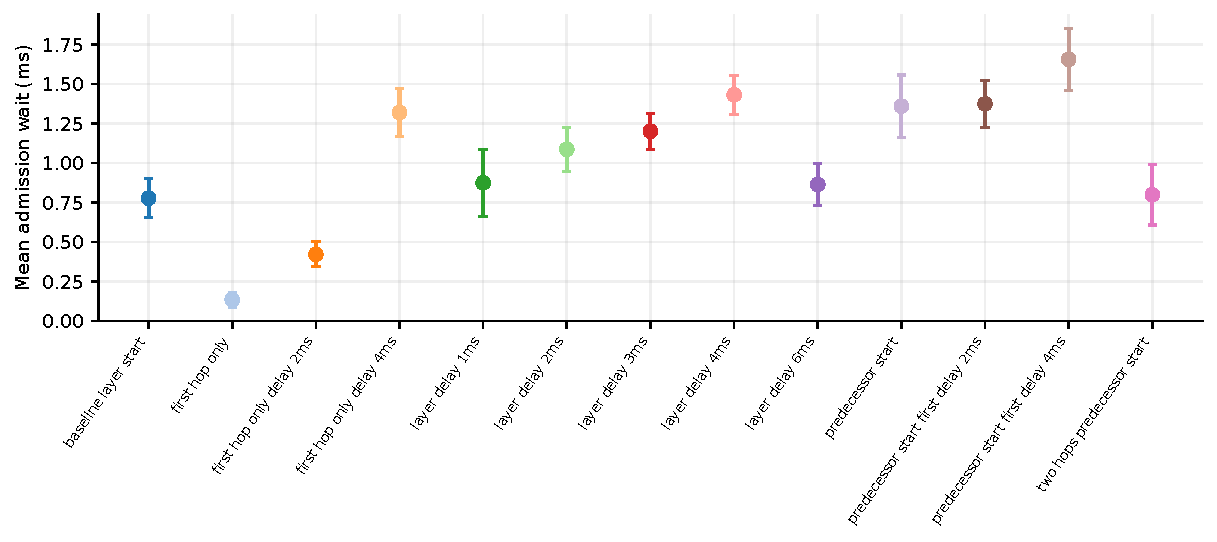
\includegraphics[width=.94\linewidth,height=.31\textheight,keepaspectratio]{figures/variants/mesh_max_reliability_average_admission_wait_ms.pdf}\captionof{figure}{Thirteen Dynamic launch variants, M=4 and C=3; zero-delay structural rules and delay sensitivities are distinguished in the definitions.}\end{center}
\begin{center}{\scriptsize\setlength{\tabcolsep}{3pt}
\begin{tabular}{lrr}
\toprule
Variant & Mean $\pm$ SD & n \\
\midrule
baseline-layer-start & $0.7779\pm0.1230$ & 6 \\
first-hop-only & $0.1357\pm0.0479$ & 6 \\
first-hop-only-delay-2ms & $0.4221\pm0.0789$ & 6 \\
first-hop-only-delay-4ms & $1.320\pm0.153$ & 6 \\
layer-delay-1ms & $0.8748\pm0.2109$ & 6 \\
layer-delay-2ms & $1.087\pm0.140$ & 6 \\
layer-delay-3ms & $1.202\pm0.115$ & 6 \\
layer-delay-4ms & $1.432\pm0.121$ & 6 \\
layer-delay-6ms & $0.8647\pm0.1329$ & 6 \\
predecessor-start & $1.361\pm0.197$ & 6 \\
predecessor-start-first-delay-2ms & $1.375\pm0.151$ & 6 \\
predecessor-start-first-delay-4ms & $1.657\pm0.196$ & 6 \\
two-hops-predecessor-start & $0.7995\pm0.1913$ & 6 \\
\bottomrule\end{tabular}}
\captionof{table}{All thirteen variants; n counts byte-distinct trace/physics runs, not conceptual aliases.}
{\footnotesize\href{https://github.com/sanjeevkrishnaa/Compiler-Driven-ACE/blob/codex/ace-scheduler-correctness/docs/latex/qft96_final/data/variants_mesh_max_reliability_average_admission_wait_ms.csv}{Exact CSV values and sample counts}}
\end{center}
\clearpage\subsection*{Delivered EPR fidelity}
\begin{center}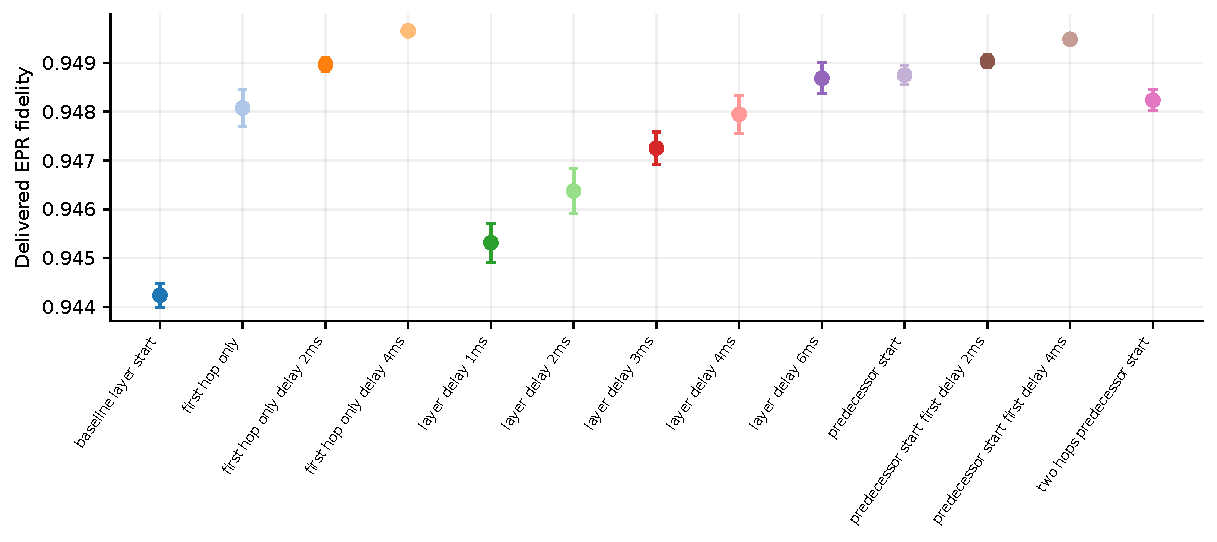
\includegraphics[width=.94\linewidth,height=.31\textheight,keepaspectratio]{figures/variants/mesh_max_reliability_average_delivered_epr_fidelity.pdf}\captionof{figure}{Thirteen Dynamic launch variants, M=4 and C=3; zero-delay structural rules and delay sensitivities are distinguished in the definitions.}\end{center}
\begin{center}{\scriptsize\setlength{\tabcolsep}{3pt}
\begin{tabular}{lrr}
\toprule
Variant & Mean $\pm$ SD & n \\
\midrule
baseline-layer-start & $0.9442\pm0.0002$ & 6 \\
first-hop-only & $0.9481\pm0.0004$ & 6 \\
first-hop-only-delay-2ms & $0.9490\pm0.0001$ & 6 \\
first-hop-only-delay-4ms & $0.9497\pm0.0000$ & 6 \\
layer-delay-1ms & $0.9453\pm0.0004$ & 6 \\
layer-delay-2ms & $0.9464\pm0.0005$ & 6 \\
layer-delay-3ms & $0.9473\pm0.0003$ & 6 \\
layer-delay-4ms & $0.9479\pm0.0004$ & 6 \\
layer-delay-6ms & $0.9487\pm0.0003$ & 6 \\
predecessor-start & $0.9488\pm0.0002$ & 6 \\
predecessor-start-first-delay-2ms & $0.9490\pm0.0001$ & 6 \\
predecessor-start-first-delay-4ms & $0.9495\pm0.0001$ & 6 \\
two-hops-predecessor-start & $0.9482\pm0.0002$ & 6 \\
\bottomrule\end{tabular}}
\captionof{table}{All thirteen variants; n counts byte-distinct trace/physics runs, not conceptual aliases.}
{\footnotesize\href{https://github.com/sanjeevkrishnaa/Compiler-Driven-ACE/blob/codex/ace-scheduler-correctness/docs/latex/qft96_final/data/variants_mesh_max_reliability_average_delivered_epr_fidelity.csv}{Exact CSV values and sample counts}}
\end{center}
\clearpage\subsection*{Compiler readiness fraction}
\begin{center}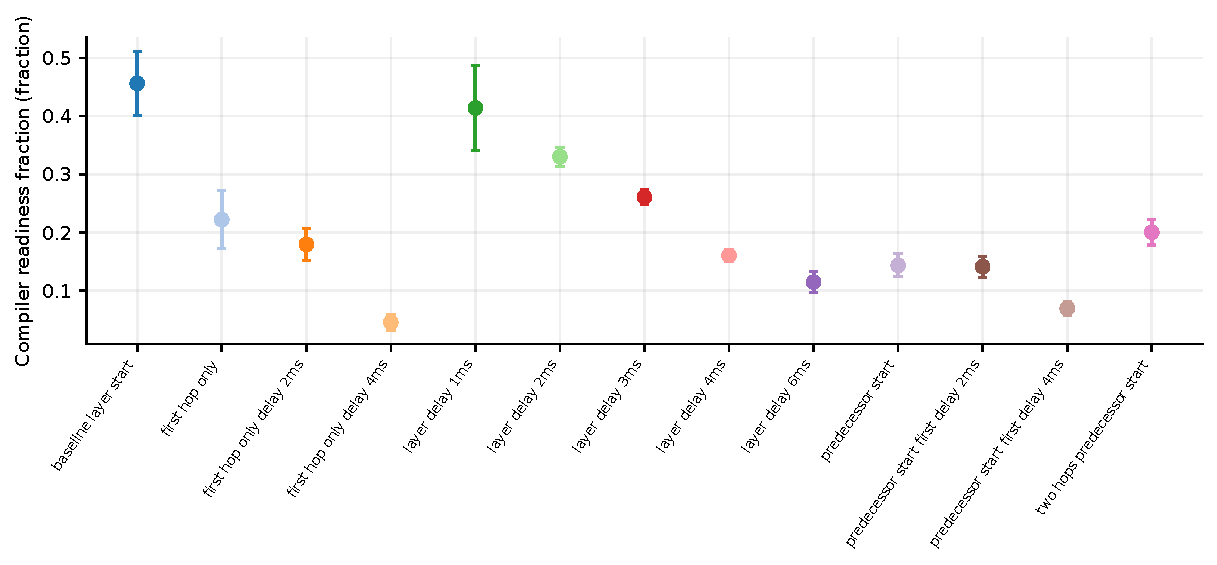
\includegraphics[width=.94\linewidth,height=.31\textheight,keepaspectratio]{figures/variants/mesh_max_reliability_pregenerated_success_rate.pdf}\captionof{figure}{Thirteen Dynamic launch variants, M=4 and C=3; zero-delay structural rules and delay sensitivities are distinguished in the definitions.}\end{center}
\begin{center}{\scriptsize\setlength{\tabcolsep}{3pt}
\begin{tabular}{lrr}
\toprule
Variant & Mean $\pm$ SD & n \\
\midrule
baseline-layer-start & $0.4564\pm0.0549$ & 6 \\
first-hop-only & $0.2219\pm0.0499$ & 6 \\
first-hop-only-delay-2ms & $0.1793\pm0.0270$ & 6 \\
first-hop-only-delay-4ms & $0.0453\pm0.0136$ & 6 \\
layer-delay-1ms & $0.4141\pm0.0731$ & 6 \\
layer-delay-2ms & $0.3301\pm0.0165$ & 6 \\
layer-delay-3ms & $0.2606\pm0.0130$ & 6 \\
layer-delay-4ms & $0.1604\pm0.0105$ & 6 \\
layer-delay-6ms & $0.1145\pm0.0179$ & 6 \\
predecessor-start & $0.1433\pm0.0197$ & 6 \\
predecessor-start-first-delay-2ms & $0.1412\pm0.0181$ & 6 \\
predecessor-start-first-delay-4ms & $0.0693\pm0.0122$ & 6 \\
two-hops-predecessor-start & $0.2004\pm0.0221$ & 6 \\
\bottomrule\end{tabular}}
\captionof{table}{All thirteen variants; n counts byte-distinct trace/physics runs, not conceptual aliases.}
{\footnotesize\href{https://github.com/sanjeevkrishnaa/Compiler-Driven-ACE/blob/codex/ace-scheduler-correctness/docs/latex/qft96_final/data/variants_mesh_max_reliability_pregenerated_success_rate.csv}{Exact CSV values and sample counts}}
\end{center}
\clearpage\subsection*{Intended compiler-hit fraction}
\begin{center}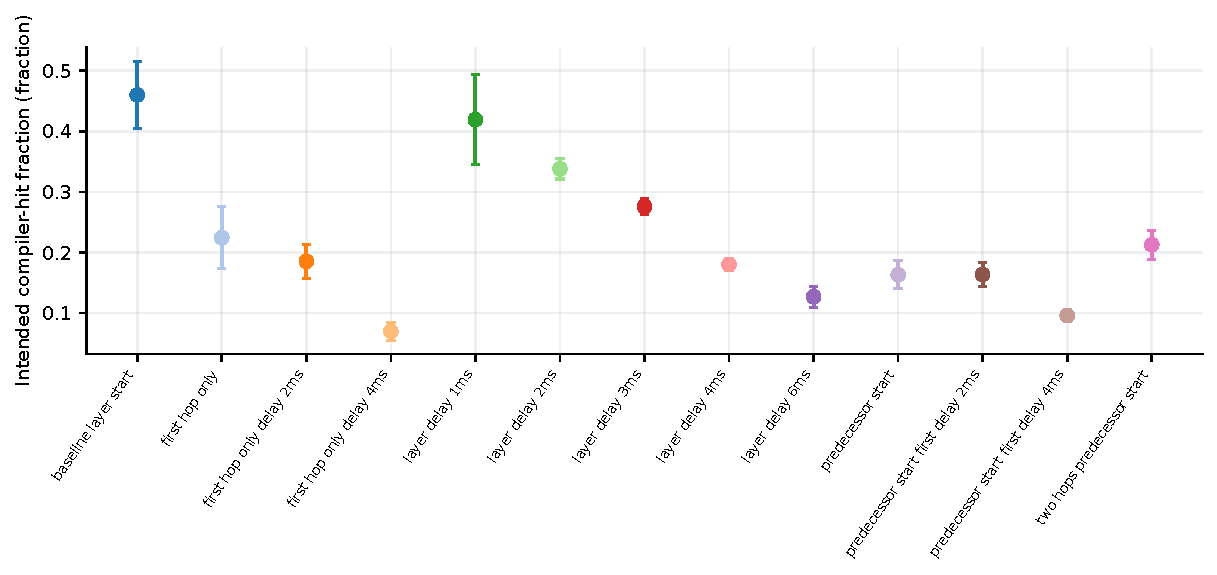
\includegraphics[width=.94\linewidth,height=.31\textheight,keepaspectratio]{figures/variants/mesh_max_reliability_intended_request_hit_rate.pdf}\captionof{figure}{Thirteen Dynamic launch variants, M=4 and C=3; zero-delay structural rules and delay sensitivities are distinguished in the definitions.}\end{center}
\begin{center}{\scriptsize\setlength{\tabcolsep}{3pt}
\begin{tabular}{lrr}
\toprule
Variant & Mean $\pm$ SD & n \\
\midrule
baseline-layer-start & $0.4600\pm0.0554$ & 6 \\
first-hop-only & $0.2246\pm0.0509$ & 6 \\
first-hop-only-delay-2ms & $0.1852\pm0.0278$ & 6 \\
first-hop-only-delay-4ms & $0.0698\pm0.0148$ & 6 \\
layer-delay-1ms & $0.4193\pm0.0741$ & 6 \\
layer-delay-2ms & $0.3380\pm0.0168$ & 6 \\
layer-delay-3ms & $0.2761\pm0.0131$ & 6 \\
layer-delay-4ms & $0.1801\pm0.0100$ & 6 \\
layer-delay-6ms & $0.1269\pm0.0174$ & 6 \\
predecessor-start & $0.1631\pm0.0231$ & 6 \\
predecessor-start-first-delay-2ms & $0.1635\pm0.0197$ & 6 \\
predecessor-start-first-delay-4ms & $0.0958\pm0.0105$ & 6 \\
two-hops-predecessor-start & $0.2126\pm0.0241$ & 6 \\
\bottomrule\end{tabular}}
\captionof{table}{All thirteen variants; n counts byte-distinct trace/physics runs, not conceptual aliases.}
{\footnotesize\href{https://github.com/sanjeevkrishnaa/Compiler-Driven-ACE/blob/codex/ace-scheduler-correctness/docs/latex/qft96_final/data/variants_mesh_max_reliability_intended_request_hit_rate.csv}{Exact CSV values and sample counts}}
\end{center}
\clearpage\subsection*{Compiler fallback fraction}
\begin{center}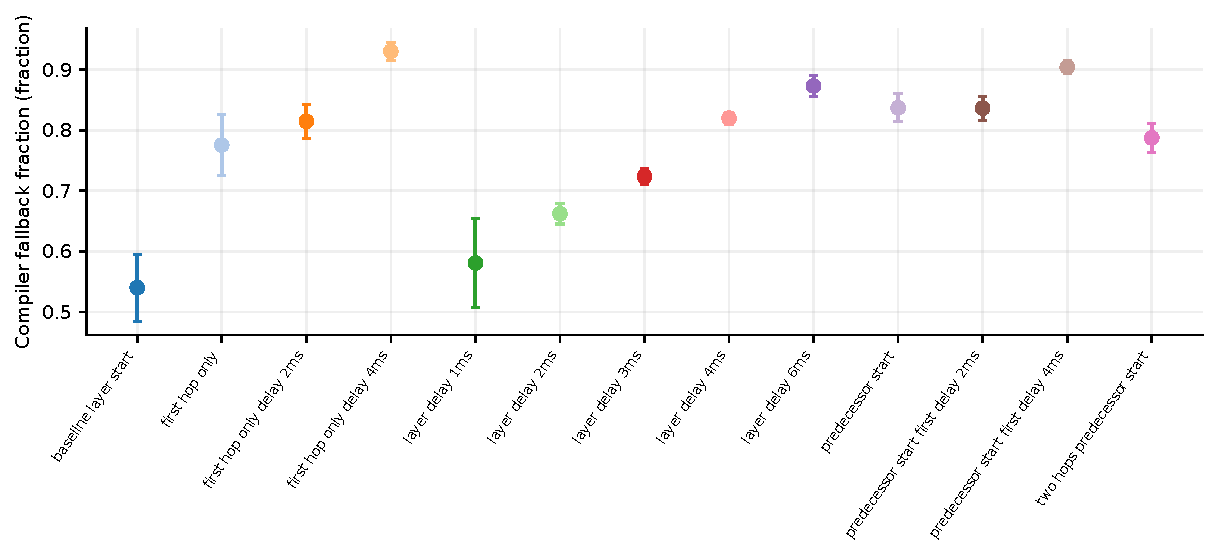
\includegraphics[width=.94\linewidth,height=.31\textheight,keepaspectratio]{figures/variants/mesh_max_reliability_on_demand_fallback_rate.pdf}\captionof{figure}{Thirteen Dynamic launch variants, M=4 and C=3; zero-delay structural rules and delay sensitivities are distinguished in the definitions.}\end{center}
\begin{center}{\scriptsize\setlength{\tabcolsep}{3pt}
\begin{tabular}{lrr}
\toprule
Variant & Mean $\pm$ SD & n \\
\midrule
baseline-layer-start & $0.5400\pm0.0554$ & 6 \\
first-hop-only & $0.7754\pm0.0509$ & 6 \\
first-hop-only-delay-2ms & $0.8148\pm0.0278$ & 6 \\
first-hop-only-delay-4ms & $0.9302\pm0.0148$ & 6 \\
layer-delay-1ms & $0.5807\pm0.0741$ & 6 \\
layer-delay-2ms & $0.6620\pm0.0168$ & 6 \\
layer-delay-3ms & $0.7239\pm0.0131$ & 6 \\
layer-delay-4ms & $0.8199\pm0.0100$ & 6 \\
layer-delay-6ms & $0.8731\pm0.0174$ & 6 \\
predecessor-start & $0.8369\pm0.0231$ & 6 \\
predecessor-start-first-delay-2ms & $0.8365\pm0.0197$ & 6 \\
predecessor-start-first-delay-4ms & $0.9042\pm0.0105$ & 6 \\
two-hops-predecessor-start & $0.7874\pm0.0241$ & 6 \\
\bottomrule\end{tabular}}
\captionof{table}{All thirteen variants; n counts byte-distinct trace/physics runs, not conceptual aliases.}
{\footnotesize\href{https://github.com/sanjeevkrishnaa/Compiler-Driven-ACE/blob/codex/ace-scheduler-correctness/docs/latex/qft96_final/data/variants_mesh_max_reliability_on_demand_fallback_rate.csv}{Exact CSV values and sample counts}}
\end{center}
\clearpage\subsection*{Compiler-cache waste}
\begin{center}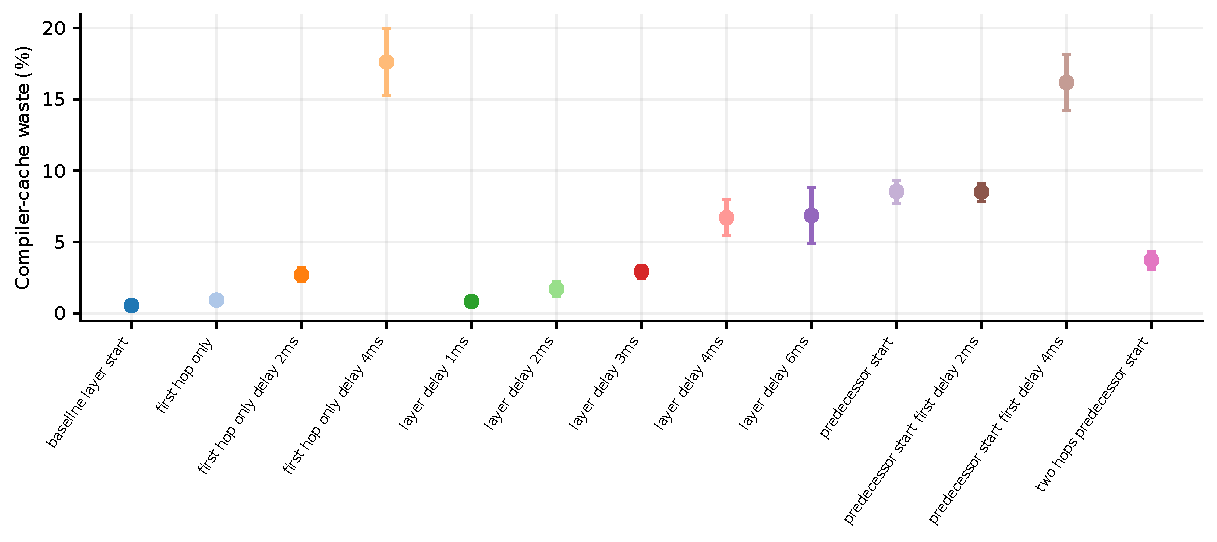
\includegraphics[width=.94\linewidth,height=.31\textheight,keepaspectratio]{figures/variants/mesh_max_reliability_compiler_waste_percentage.pdf}\captionof{figure}{Thirteen Dynamic launch variants, M=4 and C=3; zero-delay structural rules and delay sensitivities are distinguished in the definitions.}\end{center}
\begin{center}{\scriptsize\setlength{\tabcolsep}{3pt}
\begin{tabular}{lrr}
\toprule
Variant & Mean $\pm$ SD & n \\
\midrule
baseline-layer-start & $0.5427\pm0.1146$ & 6 \\
first-hop-only & $0.9258\pm0.2332$ & 6 \\
first-hop-only-delay-2ms & $2.699\pm0.488$ & 6 \\
first-hop-only-delay-4ms & $17.626\pm2.340$ & 6 \\
layer-delay-1ms & $0.8349\pm0.3123$ & 6 \\
layer-delay-2ms & $1.700\pm0.496$ & 6 \\
layer-delay-3ms & $2.928\pm0.456$ & 6 \\
layer-delay-4ms & $6.700\pm1.255$ & 6 \\
layer-delay-6ms & $6.858\pm1.973$ & 6 \\
predecessor-start & $8.530\pm0.802$ & 6 \\
predecessor-start-first-delay-2ms & $8.493\pm0.634$ & 6 \\
predecessor-start-first-delay-4ms & $16.165\pm1.966$ & 6 \\
two-hops-predecessor-start & $3.724\pm0.618$ & 6 \\
\bottomrule\end{tabular}}
\captionof{table}{All thirteen variants; n counts byte-distinct trace/physics runs, not conceptual aliases.}
{\footnotesize\href{https://github.com/sanjeevkrishnaa/Compiler-Driven-ACE/blob/codex/ace-scheduler-correctness/docs/latex/qft96_final/data/variants_mesh_max_reliability_compiler_waste_percentage.csv}{Exact CSV values and sample counts}}
\end{center}
\clearpage\subsection*{Native-protocol waste}
\begin{center}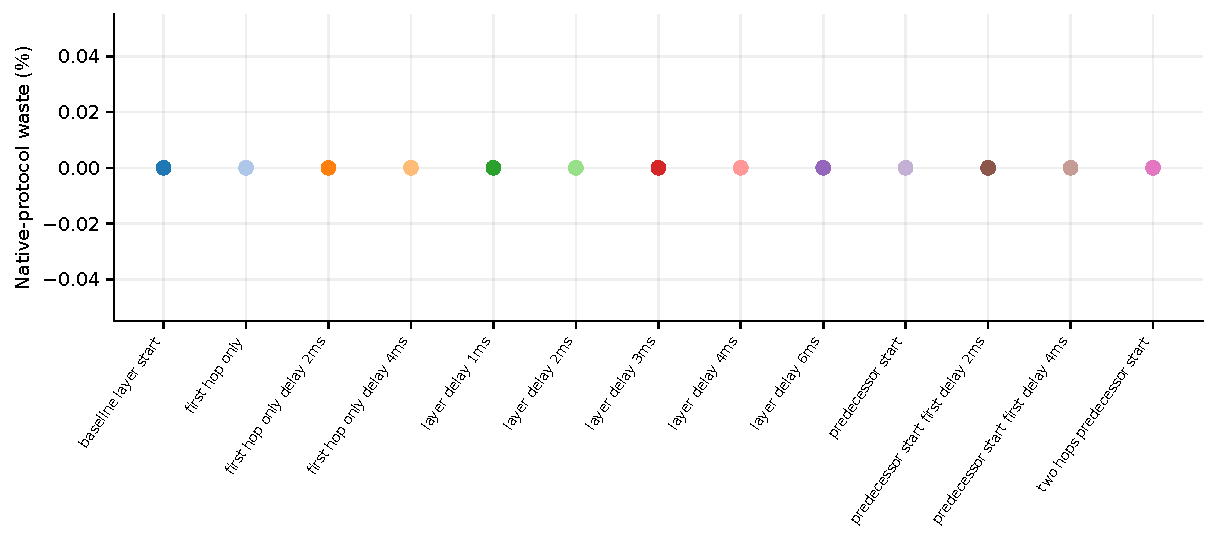
\includegraphics[width=.94\linewidth,height=.31\textheight,keepaspectratio]{figures/variants/mesh_max_reliability_protocol_waste_percentage.pdf}\captionof{figure}{Thirteen Dynamic launch variants, M=4 and C=3; zero-delay structural rules and delay sensitivities are distinguished in the definitions.}\end{center}
\begin{center}{\scriptsize\setlength{\tabcolsep}{3pt}
\begin{tabular}{lrr}
\toprule
Variant & Mean $\pm$ SD & n \\
\midrule
baseline-layer-start & $0.0000\pm0.0000$ & 6 \\
first-hop-only & $0.0000\pm0.0000$ & 6 \\
first-hop-only-delay-2ms & $0.0000\pm0.0000$ & 6 \\
first-hop-only-delay-4ms & $0.0000\pm0.0000$ & 6 \\
layer-delay-1ms & $0.0000\pm0.0000$ & 6 \\
layer-delay-2ms & $0.0000\pm0.0000$ & 6 \\
layer-delay-3ms & $0.0000\pm0.0000$ & 6 \\
layer-delay-4ms & $0.0000\pm0.0000$ & 6 \\
layer-delay-6ms & $0.0000\pm0.0000$ & 6 \\
predecessor-start & $0.0000\pm0.0000$ & 6 \\
predecessor-start-first-delay-2ms & $0.0000\pm0.0000$ & 6 \\
predecessor-start-first-delay-4ms & $0.0000\pm0.0000$ & 6 \\
two-hops-predecessor-start & $0.0000\pm0.0000$ & 6 \\
\bottomrule\end{tabular}}
\captionof{table}{All thirteen variants; n counts byte-distinct trace/physics runs, not conceptual aliases.}
{\footnotesize\href{https://github.com/sanjeevkrishnaa/Compiler-Driven-ACE/blob/codex/ace-scheduler-correctness/docs/latex/qft96_final/data/variants_mesh_max_reliability_protocol_waste_percentage.csv}{Exact CSV values and sample counts}}
\end{center}
\clearpage\subsection*{Compiler-pair expiry}
\begin{center}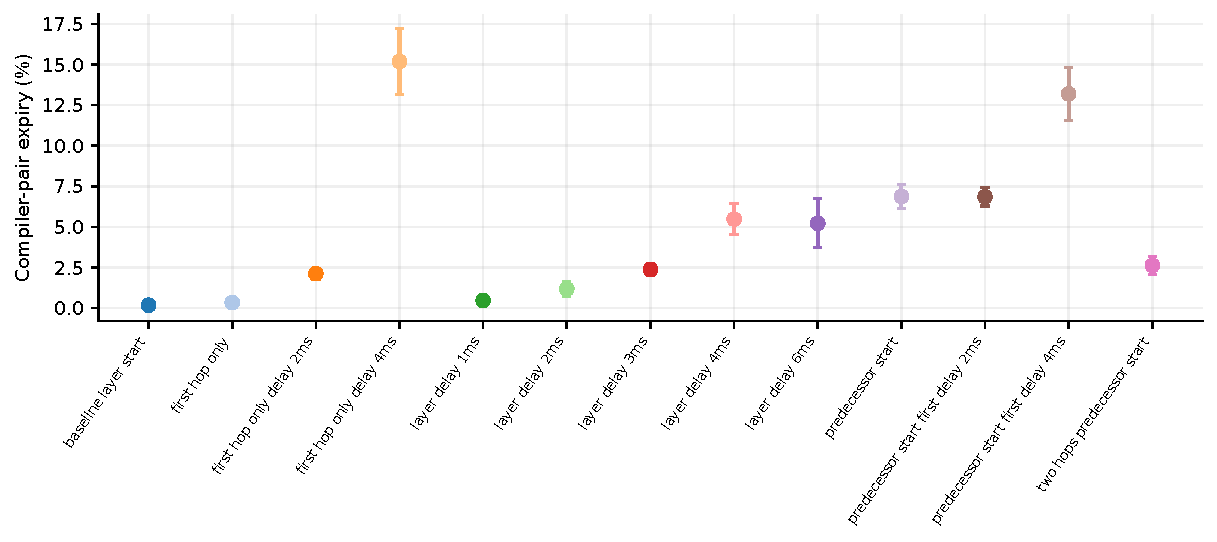
\includegraphics[width=.94\linewidth,height=.31\textheight,keepaspectratio]{figures/variants/mesh_max_reliability_compiler_expiry_percentage.pdf}\captionof{figure}{Thirteen Dynamic launch variants, M=4 and C=3; zero-delay structural rules and delay sensitivities are distinguished in the definitions.}\end{center}
\begin{center}{\scriptsize\setlength{\tabcolsep}{3pt}
\begin{tabular}{lrr}
\toprule
Variant & Mean $\pm$ SD & n \\
\midrule
baseline-layer-start & $0.1790\pm0.1236$ & 6 \\
first-hop-only & $0.3422\pm0.2835$ & 6 \\
first-hop-only-delay-2ms & $2.121\pm0.336$ & 6 \\
first-hop-only-delay-4ms & $15.175\pm2.043$ & 6 \\
layer-delay-1ms & $0.4705\pm0.2971$ & 6 \\
layer-delay-2ms & $1.181\pm0.446$ & 6 \\
layer-delay-3ms & $2.373\pm0.356$ & 6 \\
layer-delay-4ms & $5.482\pm0.963$ & 6 \\
layer-delay-6ms & $5.218\pm1.506$ & 6 \\
predecessor-start & $6.866\pm0.743$ & 6 \\
predecessor-start-first-delay-2ms & $6.844\pm0.556$ & 6 \\
predecessor-start-first-delay-4ms & $13.193\pm1.634$ & 6 \\
two-hops-predecessor-start & $2.628\pm0.532$ & 6 \\
\bottomrule\end{tabular}}
\captionof{table}{All thirteen variants; n counts byte-distinct trace/physics runs, not conceptual aliases.}
{\footnotesize\href{https://github.com/sanjeevkrishnaa/Compiler-Driven-ACE/blob/codex/ace-scheduler-correctness/docs/latex/qft96_final/data/variants_mesh_max_reliability_compiler_expiry_percentage.csv}{Exact CSV values and sample counts}}
\end{center}
\clearpage\subsection*{Used compiler-pair storage time}
\begin{center}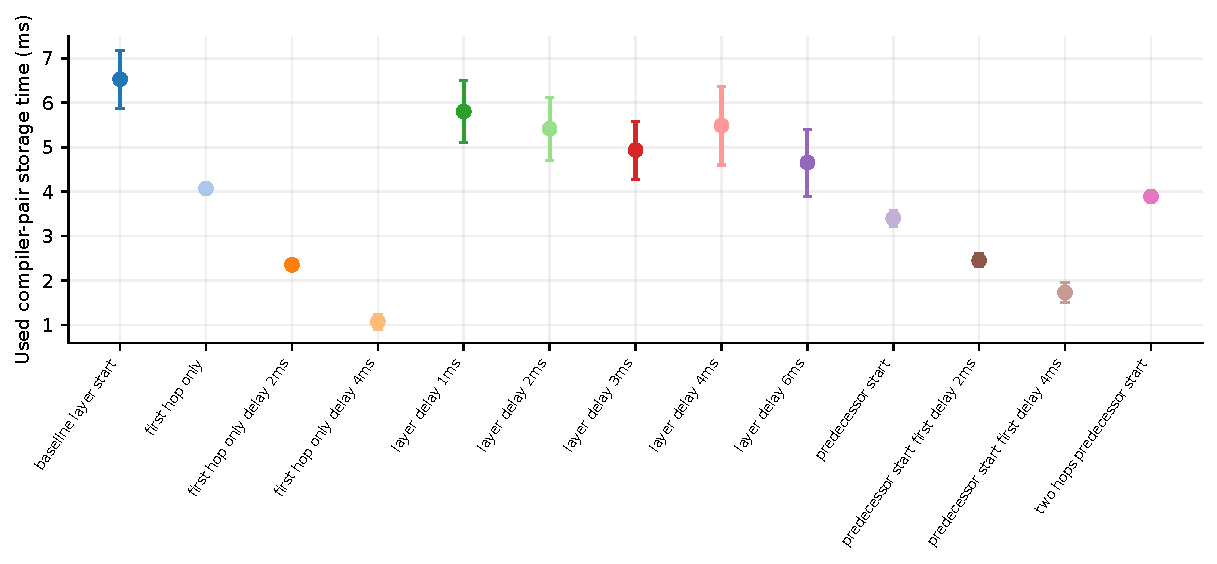
\includegraphics[width=.94\linewidth,height=.31\textheight,keepaspectratio]{figures/variants/mesh_max_reliability_average_storage_time_ms.pdf}\captionof{figure}{Thirteen Dynamic launch variants, M=4 and C=3; zero-delay structural rules and delay sensitivities are distinguished in the definitions.}\end{center}
\begin{center}{\scriptsize\setlength{\tabcolsep}{3pt}
\begin{tabular}{lrr}
\toprule
Variant & Mean $\pm$ SD & n \\
\midrule
baseline-layer-start & $6.529\pm0.649$ & 6 \\
first-hop-only & $4.070\pm0.019$ & 6 \\
first-hop-only-delay-2ms & $2.353\pm0.061$ & 6 \\
first-hop-only-delay-4ms & $1.074\pm0.170$ & 6 \\
layer-delay-1ms & $5.804\pm0.704$ & 6 \\
layer-delay-2ms & $5.415\pm0.708$ & 6 \\
layer-delay-3ms & $4.933\pm0.650$ & 6 \\
layer-delay-4ms & $5.487\pm0.887$ & 6 \\
layer-delay-6ms & $4.655\pm0.754$ & 6 \\
predecessor-start & $3.404\pm0.176$ & 6 \\
predecessor-start-first-delay-2ms & $2.452\pm0.145$ & 6 \\
predecessor-start-first-delay-4ms & $1.733\pm0.223$ & 6 \\
two-hops-predecessor-start & $3.893\pm0.098$ & 6 \\
\bottomrule\end{tabular}}
\captionof{table}{All thirteen variants; n counts byte-distinct trace/physics runs, not conceptual aliases.}
{\footnotesize\href{https://github.com/sanjeevkrishnaa/Compiler-Driven-ACE/blob/codex/ace-scheduler-correctness/docs/latex/qft96_final/data/variants_mesh_max_reliability_average_storage_time_ms.csv}{Exact CSV values and sample counts}}
\end{center}
\clearpage\subsection*{Delivered-hop throughput}
\begin{center}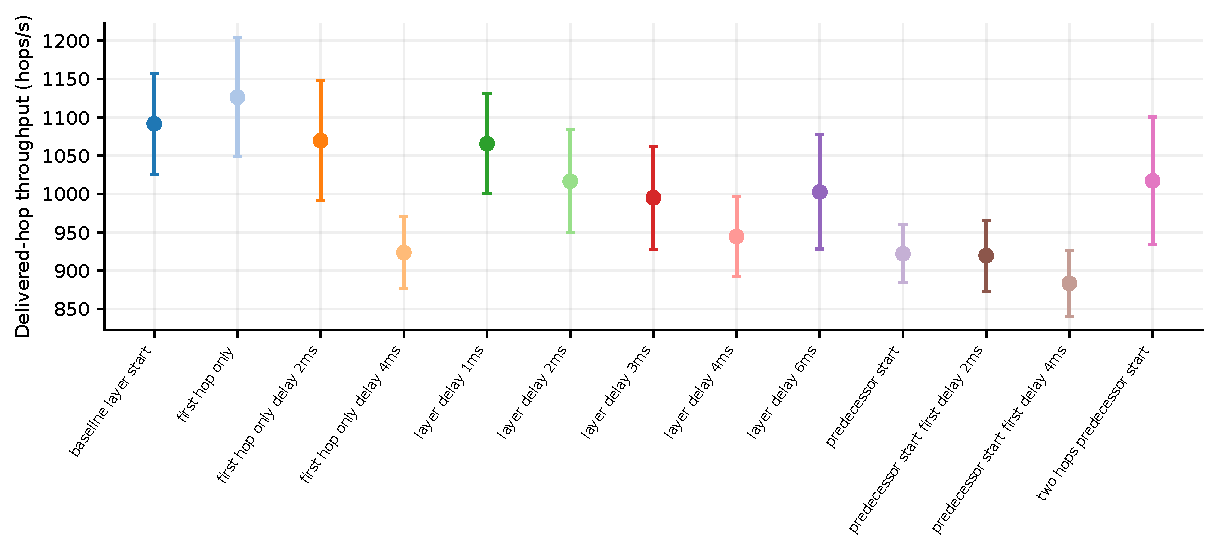
\includegraphics[width=.94\linewidth,height=.31\textheight,keepaspectratio]{figures/variants/mesh_max_reliability_hop_throughput_s.pdf}\captionof{figure}{Thirteen Dynamic launch variants, M=4 and C=3; zero-delay structural rules and delay sensitivities are distinguished in the definitions.}\end{center}
\begin{center}{\scriptsize\setlength{\tabcolsep}{3pt}
\begin{tabular}{lrr}
\toprule
Variant & Mean $\pm$ SD & n \\
\midrule
baseline-layer-start & $1091.69\pm65.83$ & 6 \\
first-hop-only & $1126.37\pm77.93$ & 6 \\
first-hop-only-delay-2ms & $1069.65\pm78.11$ & 6 \\
first-hop-only-delay-4ms & $923.78\pm46.92$ & 6 \\
layer-delay-1ms & $1065.66\pm65.05$ & 6 \\
layer-delay-2ms & $1016.74\pm67.30$ & 6 \\
layer-delay-3ms & $995.25\pm67.23$ & 6 \\
layer-delay-4ms & $944.85\pm52.56$ & 6 \\
layer-delay-6ms & $1002.81\pm74.38$ & 6 \\
predecessor-start & $922.00\pm37.76$ & 6 \\
predecessor-start-first-delay-2ms & $919.72\pm46.38$ & 6 \\
predecessor-start-first-delay-4ms & $883.61\pm42.88$ & 6 \\
two-hops-predecessor-start & $1017.30\pm83.25$ & 6 \\
\bottomrule\end{tabular}}
\captionof{table}{All thirteen variants; n counts byte-distinct trace/physics runs, not conceptual aliases.}
{\footnotesize\href{https://github.com/sanjeevkrishnaa/Compiler-Driven-ACE/blob/codex/ace-scheduler-correctness/docs/latex/qft96_final/data/variants_mesh_max_reliability_hop_throughput_s.csv}{Exact CSV values and sample counts}}
\end{center}
\clearpage\subsection*{Completion fraction}
\begin{center}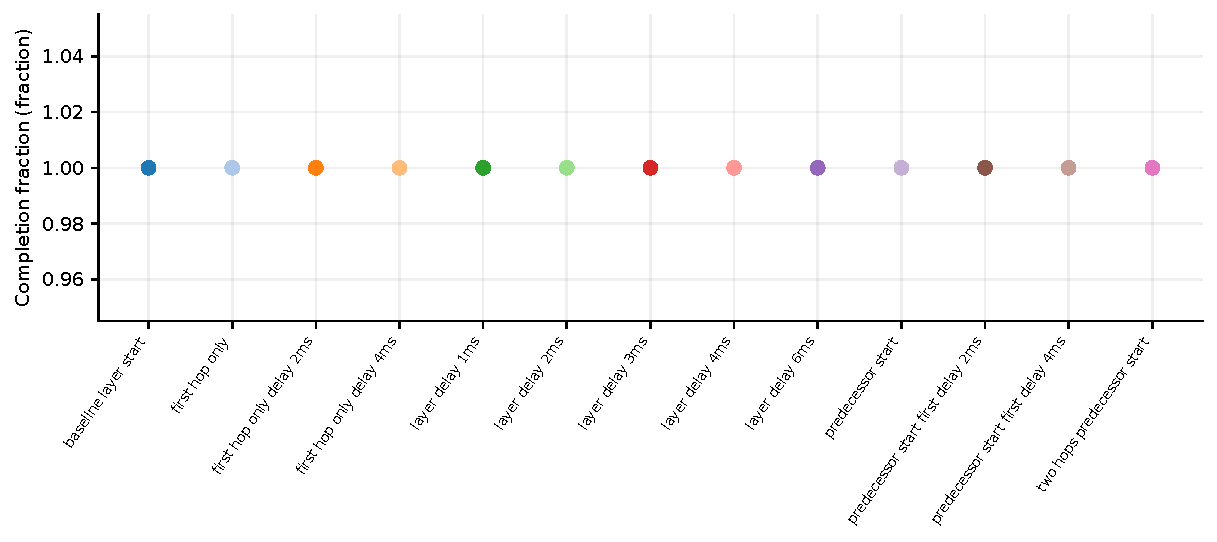
\includegraphics[width=.94\linewidth,height=.31\textheight,keepaspectratio]{figures/variants/mesh_max_reliability_completion_rate.pdf}\captionof{figure}{Thirteen Dynamic launch variants, M=4 and C=3; zero-delay structural rules and delay sensitivities are distinguished in the definitions.}\end{center}
\begin{center}{\scriptsize\setlength{\tabcolsep}{3pt}
\begin{tabular}{lrr}
\toprule
Variant & Mean $\pm$ SD & n \\
\midrule
baseline-layer-start & $1.000\pm0.000$ & 6 \\
first-hop-only & $1.000\pm0.000$ & 6 \\
first-hop-only-delay-2ms & $1.000\pm0.000$ & 6 \\
first-hop-only-delay-4ms & $1.000\pm0.000$ & 6 \\
layer-delay-1ms & $1.000\pm0.000$ & 6 \\
layer-delay-2ms & $1.000\pm0.000$ & 6 \\
layer-delay-3ms & $1.000\pm0.000$ & 6 \\
layer-delay-4ms & $1.000\pm0.000$ & 6 \\
layer-delay-6ms & $1.000\pm0.000$ & 6 \\
predecessor-start & $1.000\pm0.000$ & 6 \\
predecessor-start-first-delay-2ms & $1.000\pm0.000$ & 6 \\
predecessor-start-first-delay-4ms & $1.000\pm0.000$ & 6 \\
two-hops-predecessor-start & $1.000\pm0.000$ & 6 \\
\bottomrule\end{tabular}}
\captionof{table}{All thirteen variants; n counts byte-distinct trace/physics runs, not conceptual aliases.}
{\footnotesize\href{https://github.com/sanjeevkrishnaa/Compiler-Driven-ACE/blob/codex/ace-scheduler-correctness/docs/latex/qft96_final/data/variants_mesh_max_reliability_completion_rate.csv}{Exact CSV values and sample counts}}
\end{center}
\section{Torus / dijkstra}
\clearpage\subsection*{Mean request latency}
\begin{center}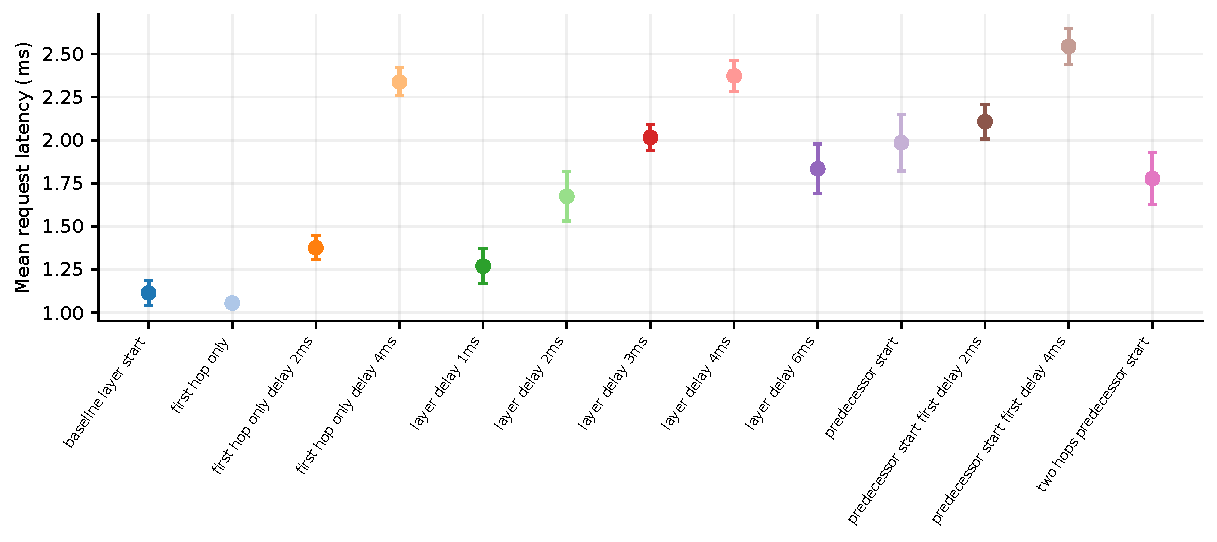
\includegraphics[width=.94\linewidth,height=.31\textheight,keepaspectratio]{figures/variants/torus_dijkstra_request_latency_mean_ms.pdf}\captionof{figure}{Thirteen Dynamic launch variants, M=4 and C=3; zero-delay structural rules and delay sensitivities are distinguished in the definitions.}\end{center}
\begin{center}{\scriptsize\setlength{\tabcolsep}{3pt}
\begin{tabular}{lrr}
\toprule
Variant & Mean $\pm$ SD & n \\
\midrule
baseline-layer-start & $1.113\pm0.073$ & 6 \\
first-hop-only & $1.054\pm0.024$ & 6 \\
first-hop-only-delay-2ms & $1.375\pm0.071$ & 6 \\
first-hop-only-delay-4ms & $2.339\pm0.081$ & 6 \\
layer-delay-1ms & $1.269\pm0.101$ & 6 \\
layer-delay-2ms & $1.674\pm0.143$ & 6 \\
layer-delay-3ms & $2.017\pm0.077$ & 6 \\
layer-delay-4ms & $2.373\pm0.089$ & 6 \\
layer-delay-6ms & $1.834\pm0.144$ & 6 \\
predecessor-start & $1.985\pm0.164$ & 6 \\
predecessor-start-first-delay-2ms & $2.107\pm0.100$ & 6 \\
predecessor-start-first-delay-4ms & $2.545\pm0.103$ & 6 \\
two-hops-predecessor-start & $1.777\pm0.153$ & 6 \\
\bottomrule\end{tabular}}
\captionof{table}{All thirteen variants; n counts byte-distinct trace/physics runs, not conceptual aliases.}
{\footnotesize\href{https://github.com/sanjeevkrishnaa/Compiler-Driven-ACE/blob/codex/ace-scheduler-correctness/docs/latex/qft96_final/data/variants_torus_dijkstra_request_latency_mean_ms.csv}{Exact CSV values and sample counts}}
\end{center}
\clearpage\subsection*{Median request latency}
\begin{center}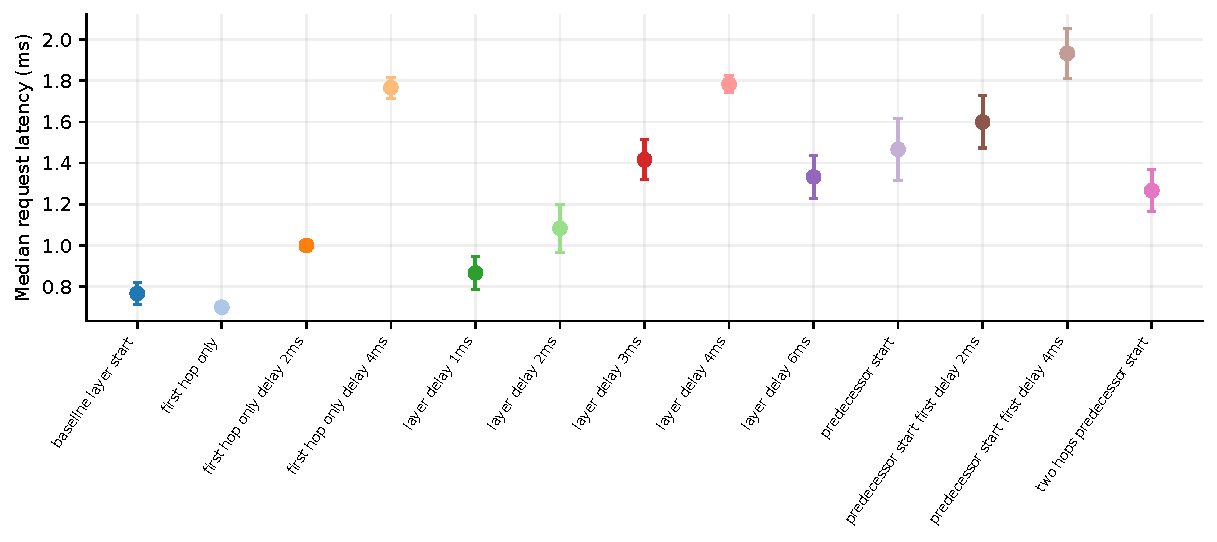
\includegraphics[width=.94\linewidth,height=.31\textheight,keepaspectratio]{figures/variants/torus_dijkstra_request_latency_median_ms.pdf}\captionof{figure}{Thirteen Dynamic launch variants, M=4 and C=3; zero-delay structural rules and delay sensitivities are distinguished in the definitions.}\end{center}
\begin{center}{\scriptsize\setlength{\tabcolsep}{3pt}
\begin{tabular}{lrr}
\toprule
Variant & Mean $\pm$ SD & n \\
\midrule
baseline-layer-start & $0.7667\pm0.0516$ & 6 \\
first-hop-only & $0.7000\pm0.0000$ & 6 \\
first-hop-only-delay-2ms & $1.000\pm0.000$ & 6 \\
first-hop-only-delay-4ms & $1.767\pm0.052$ & 6 \\
layer-delay-1ms & $0.8667\pm0.0816$ & 6 \\
layer-delay-2ms & $1.083\pm0.117$ & 6 \\
layer-delay-3ms & $1.417\pm0.098$ & 6 \\
layer-delay-4ms & $1.783\pm0.041$ & 6 \\
layer-delay-6ms & $1.333\pm0.103$ & 6 \\
predecessor-start & $1.467\pm0.151$ & 6 \\
predecessor-start-first-delay-2ms & $1.600\pm0.126$ & 6 \\
predecessor-start-first-delay-4ms & $1.933\pm0.121$ & 6 \\
two-hops-predecessor-start & $1.267\pm0.103$ & 6 \\
\bottomrule\end{tabular}}
\captionof{table}{All thirteen variants; n counts byte-distinct trace/physics runs, not conceptual aliases.}
{\footnotesize\href{https://github.com/sanjeevkrishnaa/Compiler-Driven-ACE/blob/codex/ace-scheduler-correctness/docs/latex/qft96_final/data/variants_torus_dijkstra_request_latency_median_ms.csv}{Exact CSV values and sample counts}}
\end{center}
\clearpage\subsection*{p95 request latency}
\begin{center}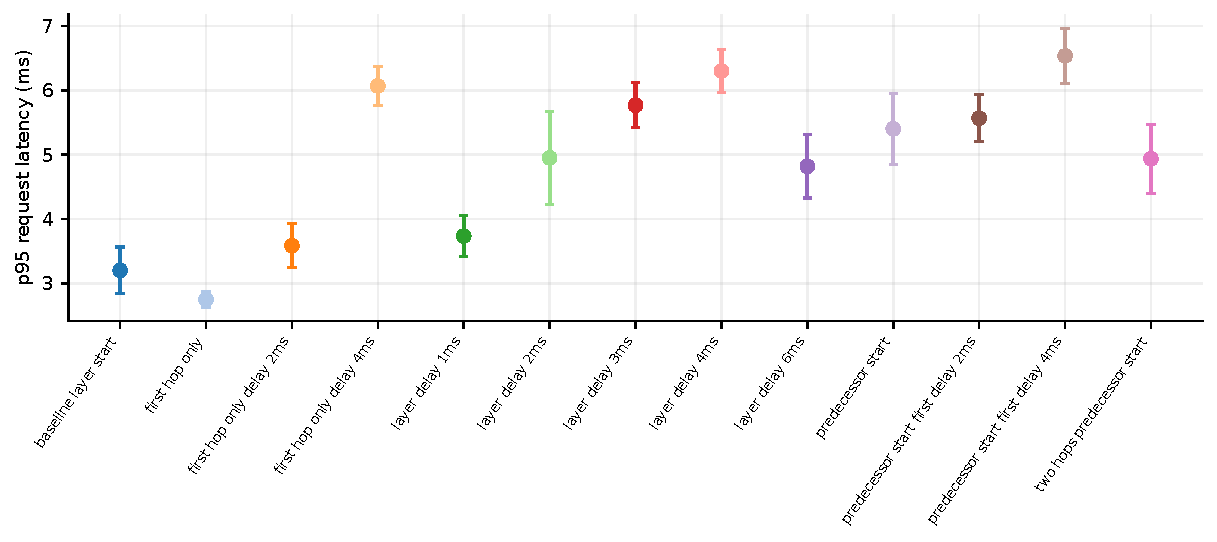
\includegraphics[width=.94\linewidth,height=.31\textheight,keepaspectratio]{figures/variants/torus_dijkstra_request_latency_p95_ms.pdf}\captionof{figure}{Thirteen Dynamic launch variants, M=4 and C=3; zero-delay structural rules and delay sensitivities are distinguished in the definitions.}\end{center}
\begin{center}{\scriptsize\setlength{\tabcolsep}{3pt}
\begin{tabular}{lrr}
\toprule
Variant & Mean $\pm$ SD & n \\
\midrule
baseline-layer-start & $3.200\pm0.363$ & 6 \\
first-hop-only & $2.750\pm0.122$ & 6 \\
first-hop-only-delay-2ms & $3.583\pm0.343$ & 6 \\
first-hop-only-delay-4ms & $6.067\pm0.308$ & 6 \\
layer-delay-1ms & $3.733\pm0.314$ & 6 \\
layer-delay-2ms & $4.950\pm0.726$ & 6 \\
layer-delay-3ms & $5.767\pm0.350$ & 6 \\
layer-delay-4ms & $6.300\pm0.329$ & 6 \\
layer-delay-6ms & $4.817\pm0.492$ & 6 \\
predecessor-start & $5.400\pm0.551$ & 6 \\
predecessor-start-first-delay-2ms & $5.567\pm0.367$ & 6 \\
predecessor-start-first-delay-4ms & $6.533\pm0.427$ & 6 \\
two-hops-predecessor-start & $4.933\pm0.532$ & 6 \\
\bottomrule\end{tabular}}
\captionof{table}{All thirteen variants; n counts byte-distinct trace/physics runs, not conceptual aliases.}
{\footnotesize\href{https://github.com/sanjeevkrishnaa/Compiler-Driven-ACE/blob/codex/ace-scheduler-correctness/docs/latex/qft96_final/data/variants_torus_dijkstra_request_latency_p95_ms.csv}{Exact CSV values and sample counts}}
\end{center}
\clearpage\subsection*{Maximum request latency}
\begin{center}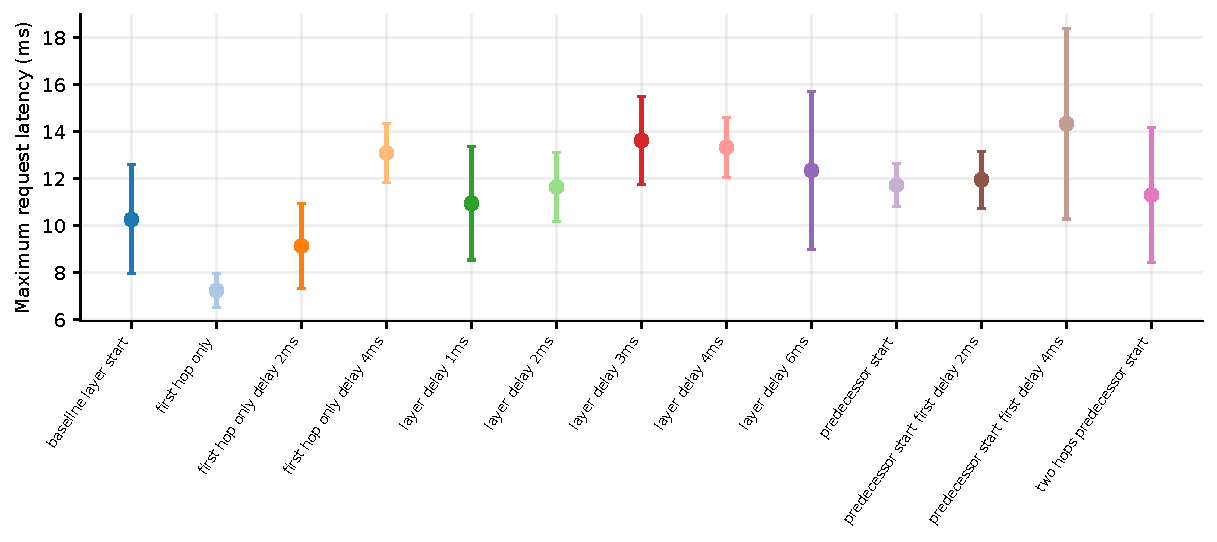
\includegraphics[width=.94\linewidth,height=.31\textheight,keepaspectratio]{figures/variants/torus_dijkstra_request_latency_max_ms.pdf}\captionof{figure}{Thirteen Dynamic launch variants, M=4 and C=3; zero-delay structural rules and delay sensitivities are distinguished in the definitions.}\end{center}
\begin{center}{\scriptsize\setlength{\tabcolsep}{3pt}
\begin{tabular}{lrr}
\toprule
Variant & Mean $\pm$ SD & n \\
\midrule
baseline-layer-start & $10.267\pm2.315$ & 6 \\
first-hop-only & $7.250\pm0.718$ & 6 \\
first-hop-only-delay-2ms & $9.134\pm1.814$ & 6 \\
first-hop-only-delay-4ms & $13.084\pm1.242$ & 6 \\
layer-delay-1ms & $10.950\pm2.411$ & 6 \\
layer-delay-2ms & $11.650\pm1.478$ & 6 \\
layer-delay-3ms & $13.617\pm1.870$ & 6 \\
layer-delay-4ms & $13.334\pm1.268$ & 6 \\
layer-delay-6ms & $12.350\pm3.361$ & 6 \\
predecessor-start & $11.734\pm0.907$ & 6 \\
predecessor-start-first-delay-2ms & $11.950\pm1.203$ & 6 \\
predecessor-start-first-delay-4ms & $14.334\pm4.051$ & 6 \\
two-hops-predecessor-start & $11.300\pm2.862$ & 6 \\
\bottomrule\end{tabular}}
\captionof{table}{All thirteen variants; n counts byte-distinct trace/physics runs, not conceptual aliases.}
{\footnotesize\href{https://github.com/sanjeevkrishnaa/Compiler-Driven-ACE/blob/codex/ace-scheduler-correctness/docs/latex/qft96_final/data/variants_torus_dijkstra_request_latency_max_ms.csv}{Exact CSV values and sample counts}}
\end{center}
\clearpage\subsection*{Communication makespan}
\begin{center}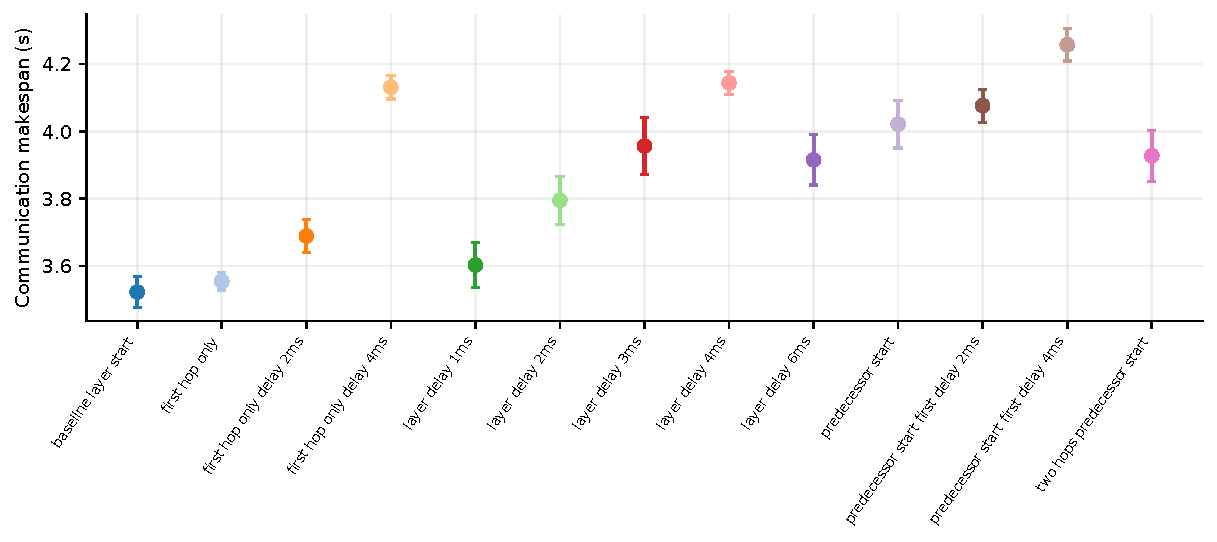
\includegraphics[width=.94\linewidth,height=.31\textheight,keepaspectratio]{figures/variants/torus_dijkstra_end_to_end_latency_ms.pdf}\captionof{figure}{Thirteen Dynamic launch variants, M=4 and C=3; zero-delay structural rules and delay sensitivities are distinguished in the definitions.}\end{center}
\begin{center}{\scriptsize\setlength{\tabcolsep}{3pt}
\begin{tabular}{lrr}
\toprule
Variant & Mean $\pm$ SD & n \\
\midrule
baseline-layer-start & $3.523\pm0.045$ & 6 \\
first-hop-only & $3.555\pm0.025$ & 6 \\
first-hop-only-delay-2ms & $3.690\pm0.050$ & 6 \\
first-hop-only-delay-4ms & $4.131\pm0.035$ & 6 \\
layer-delay-1ms & $3.603\pm0.068$ & 6 \\
layer-delay-2ms & $3.795\pm0.070$ & 6 \\
layer-delay-3ms & $3.957\pm0.085$ & 6 \\
layer-delay-4ms & $4.144\pm0.034$ & 6 \\
layer-delay-6ms & $3.916\pm0.074$ & 6 \\
predecessor-start & $4.022\pm0.071$ & 6 \\
predecessor-start-first-delay-2ms & $4.076\pm0.049$ & 6 \\
predecessor-start-first-delay-4ms & $4.258\pm0.048$ & 6 \\
two-hops-predecessor-start & $3.928\pm0.076$ & 6 \\
\bottomrule\end{tabular}}
\captionof{table}{All thirteen variants; n counts byte-distinct trace/physics runs, not conceptual aliases.}
{\footnotesize\href{https://github.com/sanjeevkrishnaa/Compiler-Driven-ACE/blob/codex/ace-scheduler-correctness/docs/latex/qft96_final/data/variants_torus_dijkstra_end_to_end_latency_ms.csv}{Exact CSV values and sample counts}}
\end{center}
\clearpage\subsection*{Mean admission wait}
\begin{center}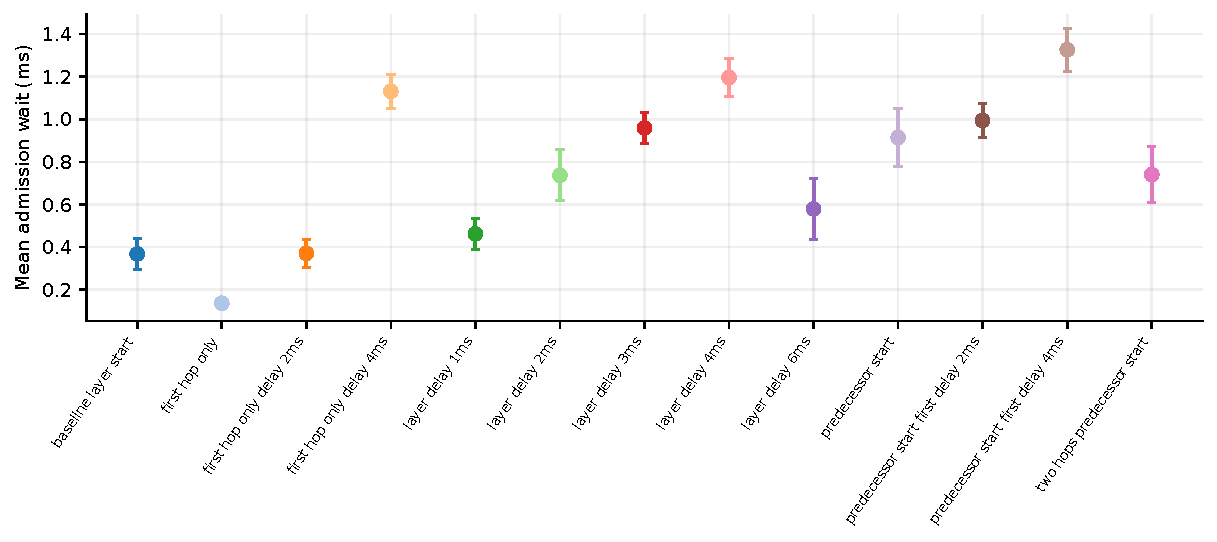
\includegraphics[width=.94\linewidth,height=.31\textheight,keepaspectratio]{figures/variants/torus_dijkstra_average_admission_wait_ms.pdf}\captionof{figure}{Thirteen Dynamic launch variants, M=4 and C=3; zero-delay structural rules and delay sensitivities are distinguished in the definitions.}\end{center}
\begin{center}{\scriptsize\setlength{\tabcolsep}{3pt}
\begin{tabular}{lrr}
\toprule
Variant & Mean $\pm$ SD & n \\
\midrule
baseline-layer-start & $0.3678\pm0.0718$ & 6 \\
first-hop-only & $0.1362\pm0.0187$ & 6 \\
first-hop-only-delay-2ms & $0.3702\pm0.0671$ & 6 \\
first-hop-only-delay-4ms & $1.131\pm0.080$ & 6 \\
layer-delay-1ms & $0.4623\pm0.0738$ & 6 \\
layer-delay-2ms & $0.7367\pm0.1197$ & 6 \\
layer-delay-3ms & $0.9587\pm0.0723$ & 6 \\
layer-delay-4ms & $1.196\pm0.088$ & 6 \\
layer-delay-6ms & $0.5792\pm0.1436$ & 6 \\
predecessor-start & $0.9144\pm0.1355$ & 6 \\
predecessor-start-first-delay-2ms & $0.9943\pm0.0818$ & 6 \\
predecessor-start-first-delay-4ms & $1.326\pm0.100$ & 6 \\
two-hops-predecessor-start & $0.7405\pm0.1304$ & 6 \\
\bottomrule\end{tabular}}
\captionof{table}{All thirteen variants; n counts byte-distinct trace/physics runs, not conceptual aliases.}
{\footnotesize\href{https://github.com/sanjeevkrishnaa/Compiler-Driven-ACE/blob/codex/ace-scheduler-correctness/docs/latex/qft96_final/data/variants_torus_dijkstra_average_admission_wait_ms.csv}{Exact CSV values and sample counts}}
\end{center}
\clearpage\subsection*{Delivered EPR fidelity}
\begin{center}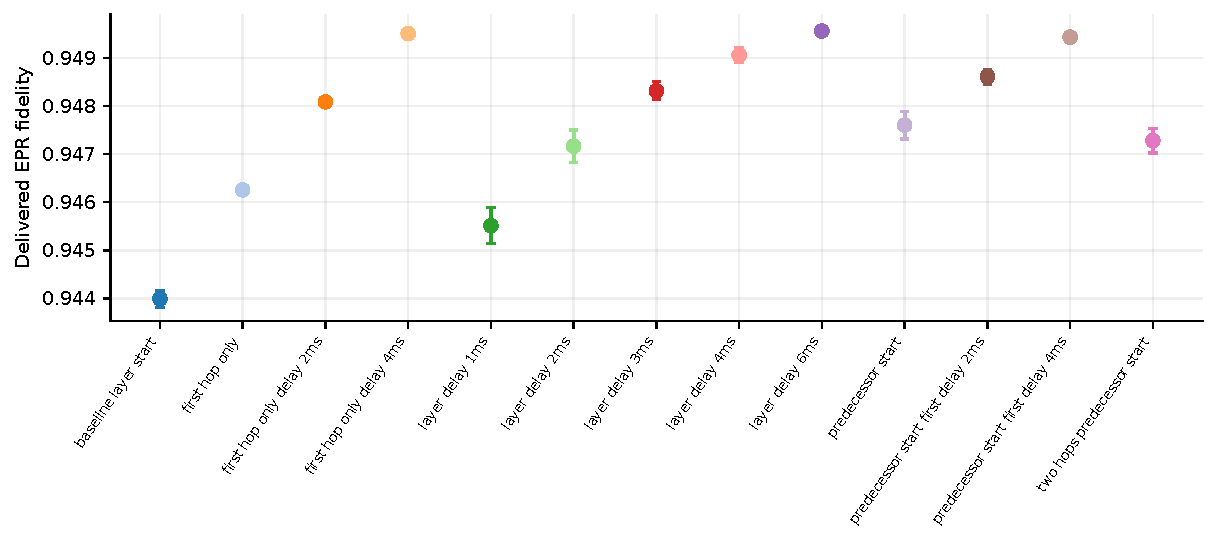
\includegraphics[width=.94\linewidth,height=.31\textheight,keepaspectratio]{figures/variants/torus_dijkstra_average_delivered_epr_fidelity.pdf}\captionof{figure}{Thirteen Dynamic launch variants, M=4 and C=3; zero-delay structural rules and delay sensitivities are distinguished in the definitions.}\end{center}
\begin{center}{\scriptsize\setlength{\tabcolsep}{3pt}
\begin{tabular}{lrr}
\toprule
Variant & Mean $\pm$ SD & n \\
\midrule
baseline-layer-start & $0.9440\pm0.0002$ & 6 \\
first-hop-only & $0.9463\pm0.0001$ & 6 \\
first-hop-only-delay-2ms & $0.9481\pm0.0001$ & 6 \\
first-hop-only-delay-4ms & $0.9495\pm0.0000$ & 6 \\
layer-delay-1ms & $0.9455\pm0.0004$ & 6 \\
layer-delay-2ms & $0.9472\pm0.0003$ & 6 \\
layer-delay-3ms & $0.9483\pm0.0002$ & 6 \\
layer-delay-4ms & $0.9491\pm0.0002$ & 6 \\
layer-delay-6ms & $0.9496\pm0.0001$ & 6 \\
predecessor-start & $0.9476\pm0.0003$ & 6 \\
predecessor-start-first-delay-2ms & $0.9486\pm0.0002$ & 6 \\
predecessor-start-first-delay-4ms & $0.9494\pm0.0000$ & 6 \\
two-hops-predecessor-start & $0.9473\pm0.0003$ & 6 \\
\bottomrule\end{tabular}}
\captionof{table}{All thirteen variants; n counts byte-distinct trace/physics runs, not conceptual aliases.}
{\footnotesize\href{https://github.com/sanjeevkrishnaa/Compiler-Driven-ACE/blob/codex/ace-scheduler-correctness/docs/latex/qft96_final/data/variants_torus_dijkstra_average_delivered_epr_fidelity.csv}{Exact CSV values and sample counts}}
\end{center}
\clearpage\subsection*{Compiler readiness fraction}
\begin{center}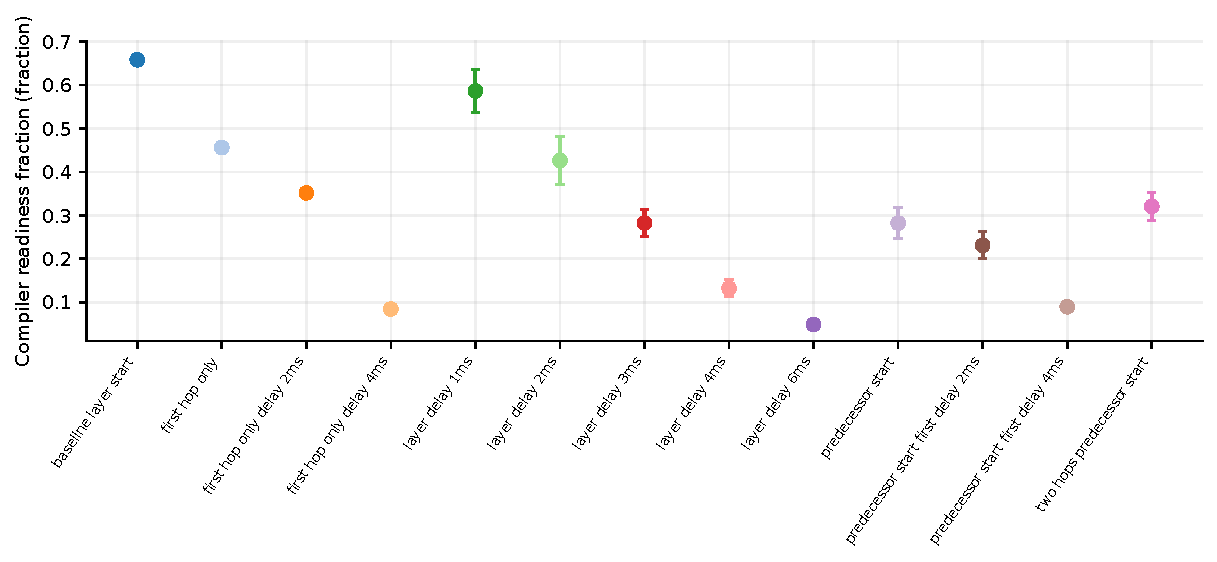
\includegraphics[width=.94\linewidth,height=.31\textheight,keepaspectratio]{figures/variants/torus_dijkstra_pregenerated_success_rate.pdf}\captionof{figure}{Thirteen Dynamic launch variants, M=4 and C=3; zero-delay structural rules and delay sensitivities are distinguished in the definitions.}\end{center}
\begin{center}{\scriptsize\setlength{\tabcolsep}{3pt}
\begin{tabular}{lrr}
\toprule
Variant & Mean $\pm$ SD & n \\
\midrule
baseline-layer-start & $0.6581\pm0.0120$ & 6 \\
first-hop-only & $0.4562\pm0.0116$ & 6 \\
first-hop-only-delay-2ms & $0.3517\pm0.0124$ & 6 \\
first-hop-only-delay-4ms & $0.0843\pm0.0089$ & 6 \\
layer-delay-1ms & $0.5864\pm0.0505$ & 6 \\
layer-delay-2ms & $0.4263\pm0.0558$ & 6 \\
layer-delay-3ms & $0.2822\pm0.0312$ & 6 \\
layer-delay-4ms & $0.1326\pm0.0192$ & 6 \\
layer-delay-6ms & $0.0486\pm0.0068$ & 6 \\
predecessor-start & $0.2823\pm0.0359$ & 6 \\
predecessor-start-first-delay-2ms & $0.2312\pm0.0310$ & 6 \\
predecessor-start-first-delay-4ms & $0.0896\pm0.0104$ & 6 \\
two-hops-predecessor-start & $0.3205\pm0.0322$ & 6 \\
\bottomrule\end{tabular}}
\captionof{table}{All thirteen variants; n counts byte-distinct trace/physics runs, not conceptual aliases.}
{\footnotesize\href{https://github.com/sanjeevkrishnaa/Compiler-Driven-ACE/blob/codex/ace-scheduler-correctness/docs/latex/qft96_final/data/variants_torus_dijkstra_pregenerated_success_rate.csv}{Exact CSV values and sample counts}}
\end{center}
\clearpage\subsection*{Intended compiler-hit fraction}
\begin{center}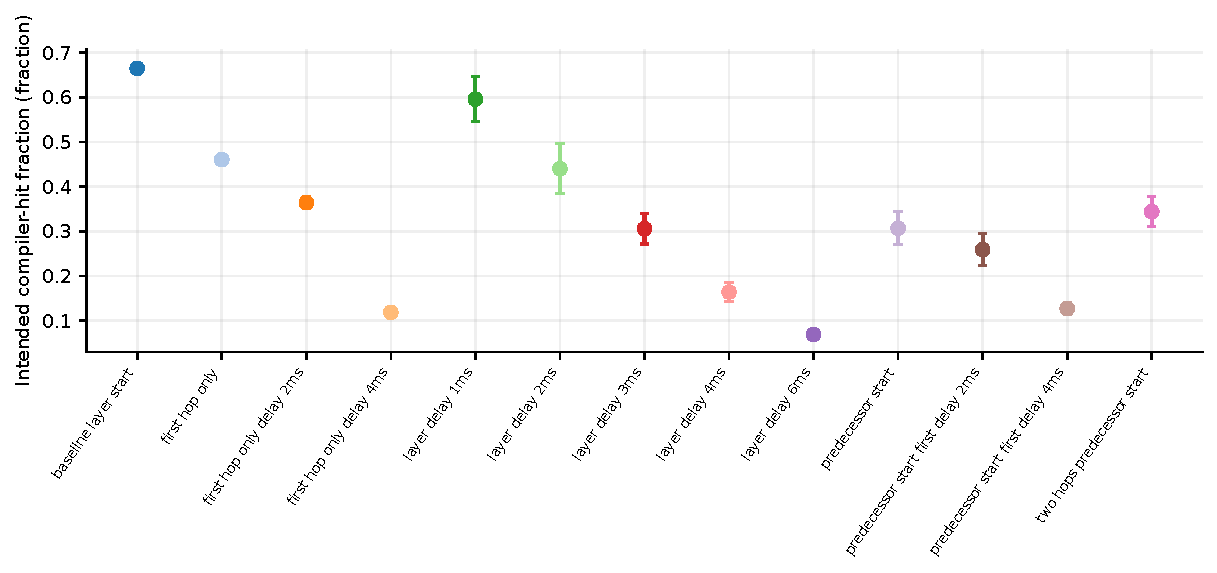
\includegraphics[width=.94\linewidth,height=.31\textheight,keepaspectratio]{figures/variants/torus_dijkstra_intended_request_hit_rate.pdf}\captionof{figure}{Thirteen Dynamic launch variants, M=4 and C=3; zero-delay structural rules and delay sensitivities are distinguished in the definitions.}\end{center}
\begin{center}{\scriptsize\setlength{\tabcolsep}{3pt}
\begin{tabular}{lrr}
\toprule
Variant & Mean $\pm$ SD & n \\
\midrule
baseline-layer-start & $0.6646\pm0.0114$ & 6 \\
first-hop-only & $0.4606\pm0.0117$ & 6 \\
first-hop-only-delay-2ms & $0.3642\pm0.0140$ & 6 \\
first-hop-only-delay-4ms & $0.1184\pm0.0096$ & 6 \\
layer-delay-1ms & $0.5958\pm0.0510$ & 6 \\
layer-delay-2ms & $0.4399\pm0.0562$ & 6 \\
layer-delay-3ms & $0.3057\pm0.0342$ & 6 \\
layer-delay-4ms & $0.1641\pm0.0221$ & 6 \\
layer-delay-6ms & $0.0689\pm0.0087$ & 6 \\
predecessor-start & $0.3068\pm0.0370$ & 6 \\
predecessor-start-first-delay-2ms & $0.2588\pm0.0354$ & 6 \\
predecessor-start-first-delay-4ms & $0.1271\pm0.0135$ & 6 \\
two-hops-predecessor-start & $0.3439\pm0.0338$ & 6 \\
\bottomrule\end{tabular}}
\captionof{table}{All thirteen variants; n counts byte-distinct trace/physics runs, not conceptual aliases.}
{\footnotesize\href{https://github.com/sanjeevkrishnaa/Compiler-Driven-ACE/blob/codex/ace-scheduler-correctness/docs/latex/qft96_final/data/variants_torus_dijkstra_intended_request_hit_rate.csv}{Exact CSV values and sample counts}}
\end{center}
\clearpage\subsection*{Compiler fallback fraction}
\begin{center}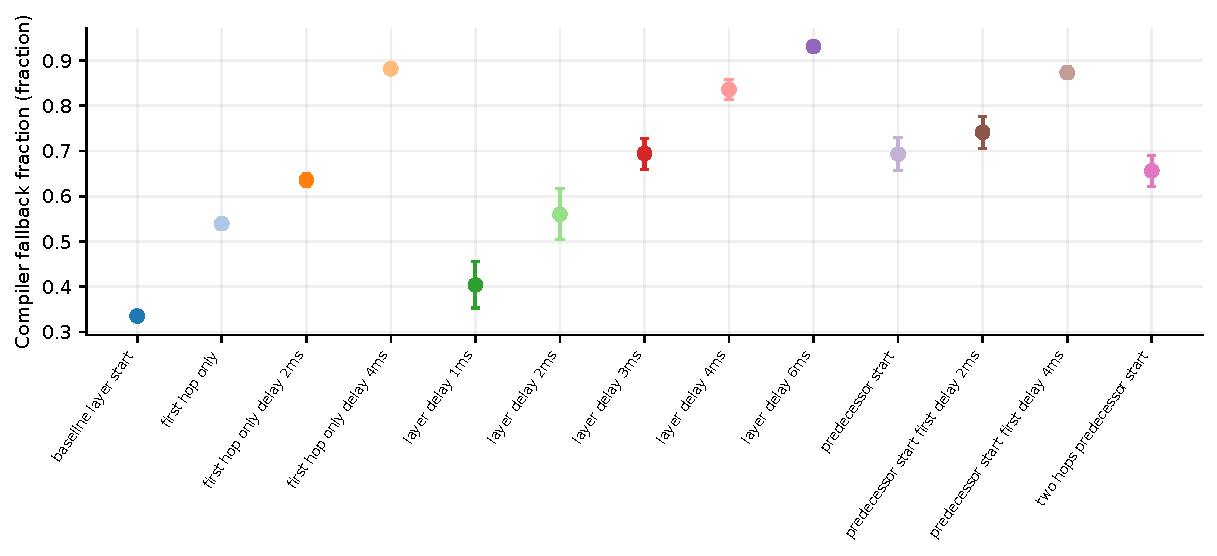
\includegraphics[width=.94\linewidth,height=.31\textheight,keepaspectratio]{figures/variants/torus_dijkstra_on_demand_fallback_rate.pdf}\captionof{figure}{Thirteen Dynamic launch variants, M=4 and C=3; zero-delay structural rules and delay sensitivities are distinguished in the definitions.}\end{center}
\begin{center}{\scriptsize\setlength{\tabcolsep}{3pt}
\begin{tabular}{lrr}
\toprule
Variant & Mean $\pm$ SD & n \\
\midrule
baseline-layer-start & $0.3354\pm0.0114$ & 6 \\
first-hop-only & $0.5394\pm0.0117$ & 6 \\
first-hop-only-delay-2ms & $0.6358\pm0.0140$ & 6 \\
first-hop-only-delay-4ms & $0.8816\pm0.0096$ & 6 \\
layer-delay-1ms & $0.4042\pm0.0510$ & 6 \\
layer-delay-2ms & $0.5601\pm0.0562$ & 6 \\
layer-delay-3ms & $0.6943\pm0.0342$ & 6 \\
layer-delay-4ms & $0.8359\pm0.0221$ & 6 \\
layer-delay-6ms & $0.9311\pm0.0087$ & 6 \\
predecessor-start & $0.6932\pm0.0370$ & 6 \\
predecessor-start-first-delay-2ms & $0.7412\pm0.0354$ & 6 \\
predecessor-start-first-delay-4ms & $0.8729\pm0.0135$ & 6 \\
two-hops-predecessor-start & $0.6561\pm0.0338$ & 6 \\
\bottomrule\end{tabular}}
\captionof{table}{All thirteen variants; n counts byte-distinct trace/physics runs, not conceptual aliases.}
{\footnotesize\href{https://github.com/sanjeevkrishnaa/Compiler-Driven-ACE/blob/codex/ace-scheduler-correctness/docs/latex/qft96_final/data/variants_torus_dijkstra_on_demand_fallback_rate.csv}{Exact CSV values and sample counts}}
\end{center}
\clearpage\subsection*{Compiler-cache waste}
\begin{center}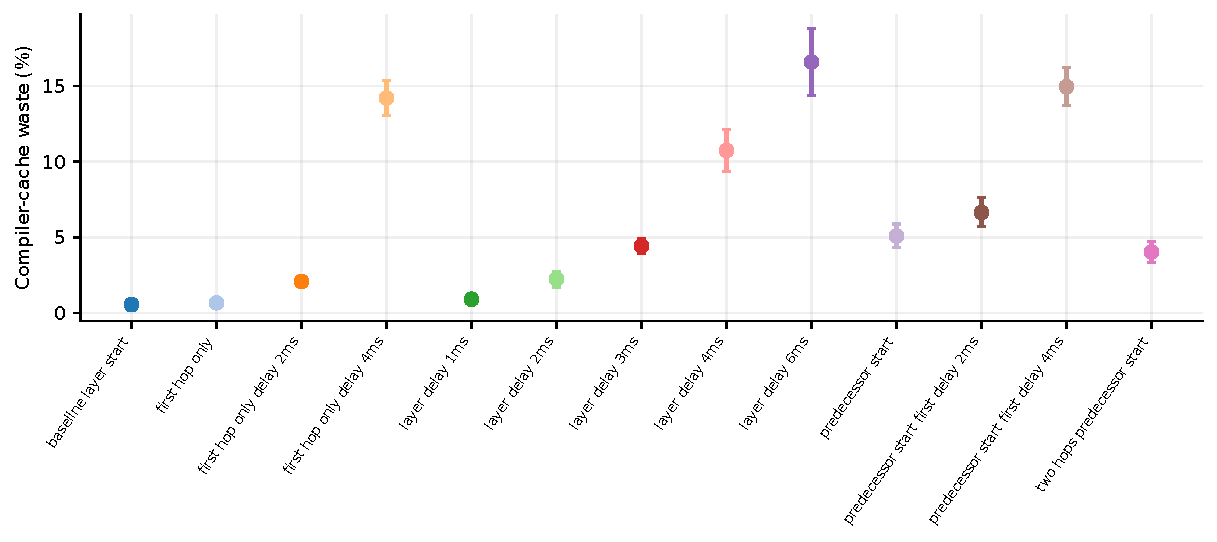
\includegraphics[width=.94\linewidth,height=.31\textheight,keepaspectratio]{figures/variants/torus_dijkstra_compiler_waste_percentage.pdf}\captionof{figure}{Thirteen Dynamic launch variants, M=4 and C=3; zero-delay structural rules and delay sensitivities are distinguished in the definitions.}\end{center}
\begin{center}{\scriptsize\setlength{\tabcolsep}{3pt}
\begin{tabular}{lrr}
\toprule
Variant & Mean $\pm$ SD & n \\
\midrule
baseline-layer-start & $0.5420\pm0.1678$ & 6 \\
first-hop-only & $0.6647\pm0.1258$ & 6 \\
first-hop-only-delay-2ms & $2.086\pm0.285$ & 6 \\
first-hop-only-delay-4ms & $14.205\pm1.180$ & 6 \\
layer-delay-1ms & $0.8995\pm0.3274$ & 6 \\
layer-delay-2ms & $2.238\pm0.525$ & 6 \\
layer-delay-3ms & $4.411\pm0.508$ & 6 \\
layer-delay-4ms & $10.733\pm1.386$ & 6 \\
layer-delay-6ms & $16.591\pm2.221$ & 6 \\
predecessor-start & $5.089\pm0.788$ & 6 \\
predecessor-start-first-delay-2ms & $6.650\pm0.951$ & 6 \\
predecessor-start-first-delay-4ms & $14.954\pm1.247$ & 6 \\
two-hops-predecessor-start & $4.030\pm0.696$ & 6 \\
\bottomrule\end{tabular}}
\captionof{table}{All thirteen variants; n counts byte-distinct trace/physics runs, not conceptual aliases.}
{\footnotesize\href{https://github.com/sanjeevkrishnaa/Compiler-Driven-ACE/blob/codex/ace-scheduler-correctness/docs/latex/qft96_final/data/variants_torus_dijkstra_compiler_waste_percentage.csv}{Exact CSV values and sample counts}}
\end{center}
\clearpage\subsection*{Native-protocol waste}
\begin{center}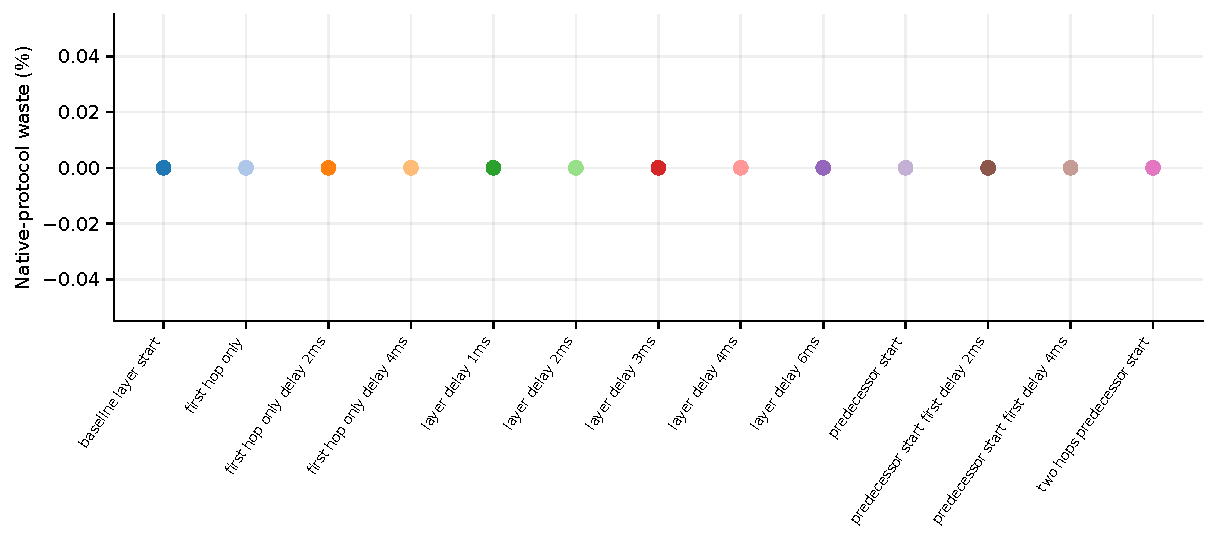
\includegraphics[width=.94\linewidth,height=.31\textheight,keepaspectratio]{figures/variants/torus_dijkstra_protocol_waste_percentage.pdf}\captionof{figure}{Thirteen Dynamic launch variants, M=4 and C=3; zero-delay structural rules and delay sensitivities are distinguished in the definitions.}\end{center}
\begin{center}{\scriptsize\setlength{\tabcolsep}{3pt}
\begin{tabular}{lrr}
\toprule
Variant & Mean $\pm$ SD & n \\
\midrule
baseline-layer-start & $0.0000\pm0.0000$ & 6 \\
first-hop-only & $0.0000\pm0.0000$ & 6 \\
first-hop-only-delay-2ms & $0.0000\pm0.0000$ & 6 \\
first-hop-only-delay-4ms & $0.0000\pm0.0000$ & 6 \\
layer-delay-1ms & $0.0000\pm0.0000$ & 6 \\
layer-delay-2ms & $0.0000\pm0.0000$ & 6 \\
layer-delay-3ms & $0.0000\pm0.0000$ & 6 \\
layer-delay-4ms & $0.0000\pm0.0000$ & 6 \\
layer-delay-6ms & $0.0000\pm0.0000$ & 6 \\
predecessor-start & $0.0000\pm0.0000$ & 6 \\
predecessor-start-first-delay-2ms & $0.0000\pm0.0000$ & 6 \\
predecessor-start-first-delay-4ms & $0.0000\pm0.0000$ & 6 \\
two-hops-predecessor-start & $0.0000\pm0.0000$ & 6 \\
\bottomrule\end{tabular}}
\captionof{table}{All thirteen variants; n counts byte-distinct trace/physics runs, not conceptual aliases.}
{\footnotesize\href{https://github.com/sanjeevkrishnaa/Compiler-Driven-ACE/blob/codex/ace-scheduler-correctness/docs/latex/qft96_final/data/variants_torus_dijkstra_protocol_waste_percentage.csv}{Exact CSV values and sample counts}}
\end{center}
\clearpage\subsection*{Compiler-pair expiry}
\begin{center}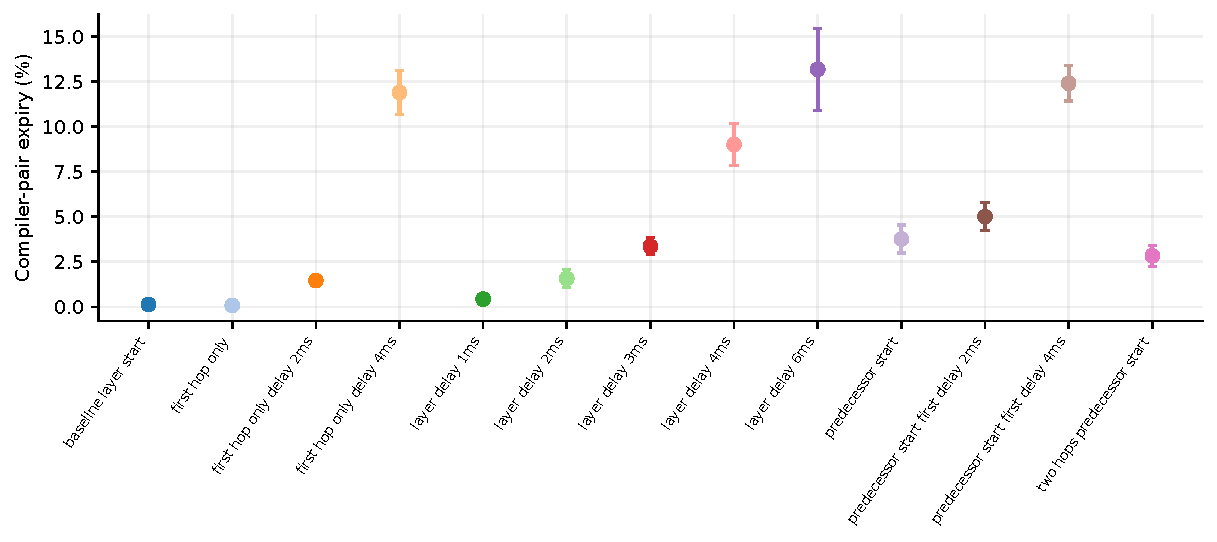
\includegraphics[width=.94\linewidth,height=.31\textheight,keepaspectratio]{figures/variants/torus_dijkstra_compiler_expiry_percentage.pdf}\captionof{figure}{Thirteen Dynamic launch variants, M=4 and C=3; zero-delay structural rules and delay sensitivities are distinguished in the definitions.}\end{center}
\begin{center}{\scriptsize\setlength{\tabcolsep}{3pt}
\begin{tabular}{lrr}
\toprule
Variant & Mean $\pm$ SD & n \\
\midrule
baseline-layer-start & $0.1267\pm0.1472$ & 6 \\
first-hop-only & $0.0780\pm0.0657$ & 6 \\
first-hop-only-delay-2ms & $1.455\pm0.227$ & 6 \\
first-hop-only-delay-4ms & $11.890\pm1.202$ & 6 \\
layer-delay-1ms & $0.4311\pm0.2370$ & 6 \\
layer-delay-2ms & $1.573\pm0.503$ & 6 \\
layer-delay-3ms & $3.361\pm0.469$ & 6 \\
layer-delay-4ms & $9.006\pm1.151$ & 6 \\
layer-delay-6ms & $13.179\pm2.269$ & 6 \\
predecessor-start & $3.764\pm0.777$ & 6 \\
predecessor-start-first-delay-2ms & $5.005\pm0.778$ & 6 \\
predecessor-start-first-delay-4ms & $12.407\pm0.984$ & 6 \\
two-hops-predecessor-start & $2.832\pm0.578$ & 6 \\
\bottomrule\end{tabular}}
\captionof{table}{All thirteen variants; n counts byte-distinct trace/physics runs, not conceptual aliases.}
{\footnotesize\href{https://github.com/sanjeevkrishnaa/Compiler-Driven-ACE/blob/codex/ace-scheduler-correctness/docs/latex/qft96_final/data/variants_torus_dijkstra_compiler_expiry_percentage.csv}{Exact CSV values and sample counts}}
\end{center}
\clearpage\subsection*{Used compiler-pair storage time}
\begin{center}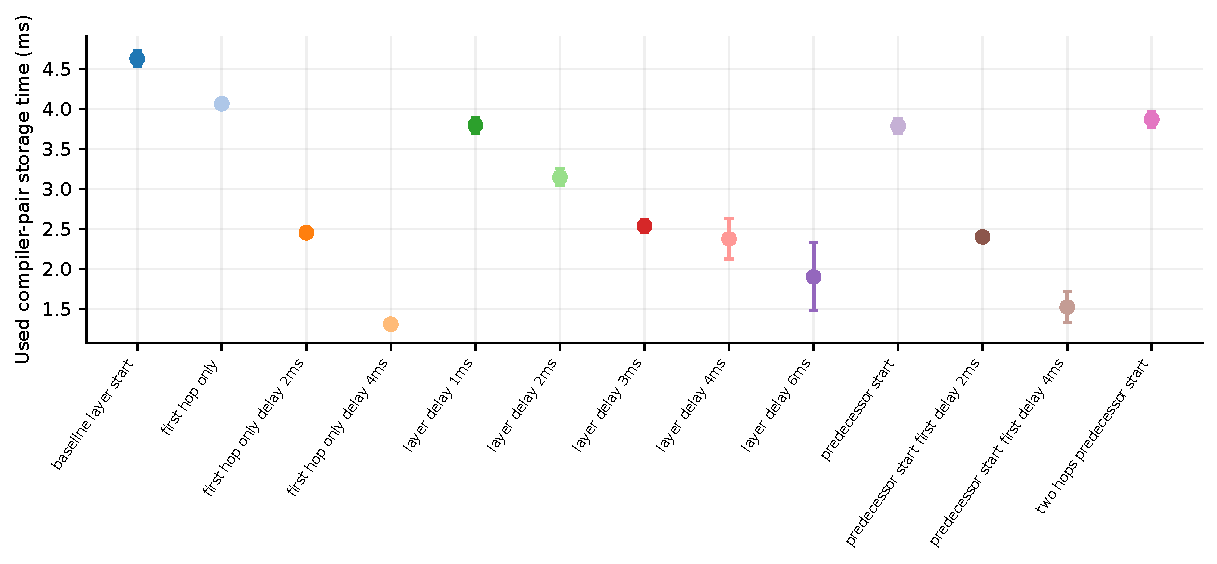
\includegraphics[width=.94\linewidth,height=.31\textheight,keepaspectratio]{figures/variants/torus_dijkstra_average_storage_time_ms.pdf}\captionof{figure}{Thirteen Dynamic launch variants, M=4 and C=3; zero-delay structural rules and delay sensitivities are distinguished in the definitions.}\end{center}
\begin{center}{\scriptsize\setlength{\tabcolsep}{3pt}
\begin{tabular}{lrr}
\toprule
Variant & Mean $\pm$ SD & n \\
\midrule
baseline-layer-start & $4.629\pm0.102$ & 6 \\
first-hop-only & $4.064\pm0.038$ & 6 \\
first-hop-only-delay-2ms & $2.453\pm0.052$ & 6 \\
first-hop-only-delay-4ms & $1.309\pm0.062$ & 6 \\
layer-delay-1ms & $3.795\pm0.099$ & 6 \\
layer-delay-2ms & $3.147\pm0.103$ & 6 \\
layer-delay-3ms & $2.538\pm0.085$ & 6 \\
layer-delay-4ms & $2.375\pm0.250$ & 6 \\
layer-delay-6ms & $1.901\pm0.424$ & 6 \\
predecessor-start & $3.785\pm0.095$ & 6 \\
predecessor-start-first-delay-2ms & $2.401\pm0.055$ & 6 \\
predecessor-start-first-delay-4ms & $1.524\pm0.190$ & 6 \\
two-hops-predecessor-start & $3.870\pm0.095$ & 6 \\
\bottomrule\end{tabular}}
\captionof{table}{All thirteen variants; n counts byte-distinct trace/physics runs, not conceptual aliases.}
{\footnotesize\href{https://github.com/sanjeevkrishnaa/Compiler-Driven-ACE/blob/codex/ace-scheduler-correctness/docs/latex/qft96_final/data/variants_torus_dijkstra_average_storage_time_ms.csv}{Exact CSV values and sample counts}}
\end{center}
\clearpage\subsection*{Delivered-hop throughput}
\begin{center}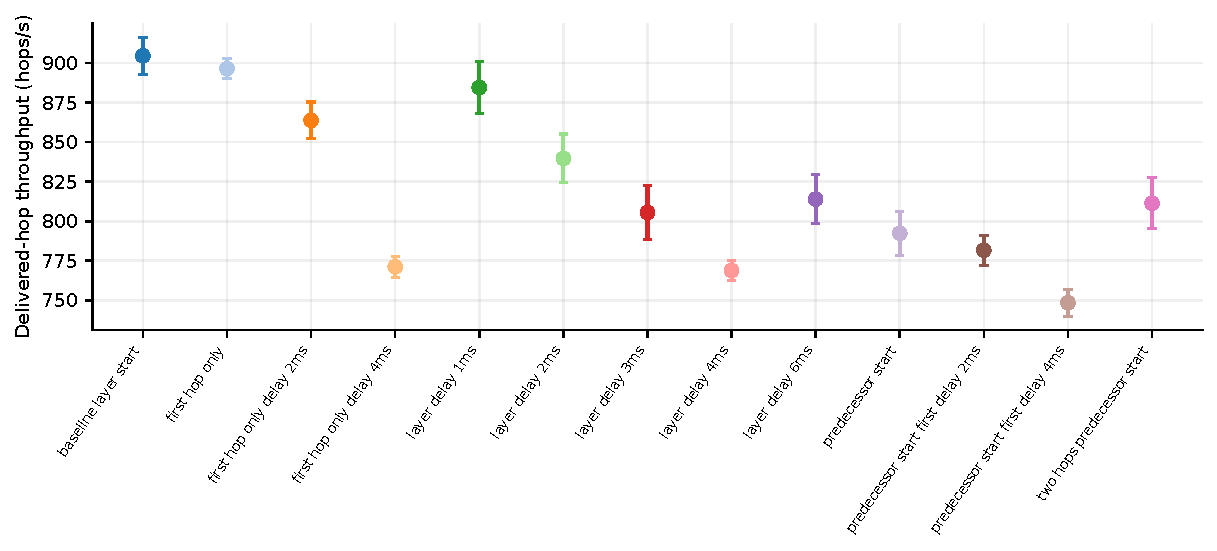
\includegraphics[width=.94\linewidth,height=.31\textheight,keepaspectratio]{figures/variants/torus_dijkstra_hop_throughput_s.pdf}\captionof{figure}{Thirteen Dynamic launch variants, M=4 and C=3; zero-delay structural rules and delay sensitivities are distinguished in the definitions.}\end{center}
\begin{center}{\scriptsize\setlength{\tabcolsep}{3pt}
\begin{tabular}{lrr}
\toprule
Variant & Mean $\pm$ SD & n \\
\midrule
baseline-layer-start & $904.41\pm11.66$ & 6 \\
first-hop-only & $896.32\pm6.42$ & 6 \\
first-hop-only-delay-2ms & $863.66\pm11.66$ & 6 \\
first-hop-only-delay-4ms & $771.21\pm6.56$ & 6 \\
layer-delay-1ms & $884.43\pm16.57$ & 6 \\
layer-delay-2ms & $839.66\pm15.43$ & 6 \\
layer-delay-3ms & $805.43\pm17.17$ & 6 \\
layer-delay-4ms & $768.89\pm6.20$ & 6 \\
layer-delay-6ms & $813.92\pm15.46$ & 6 \\
predecessor-start & $792.41\pm13.98$ & 6 \\
predecessor-start-first-delay-2ms & $781.66\pm9.51$ & 6 \\
predecessor-start-first-delay-4ms & $748.40\pm8.43$ & 6 \\
two-hops-predecessor-start & $811.45\pm16.08$ & 6 \\
\bottomrule\end{tabular}}
\captionof{table}{All thirteen variants; n counts byte-distinct trace/physics runs, not conceptual aliases.}
{\footnotesize\href{https://github.com/sanjeevkrishnaa/Compiler-Driven-ACE/blob/codex/ace-scheduler-correctness/docs/latex/qft96_final/data/variants_torus_dijkstra_hop_throughput_s.csv}{Exact CSV values and sample counts}}
\end{center}
\clearpage\subsection*{Completion fraction}
\begin{center}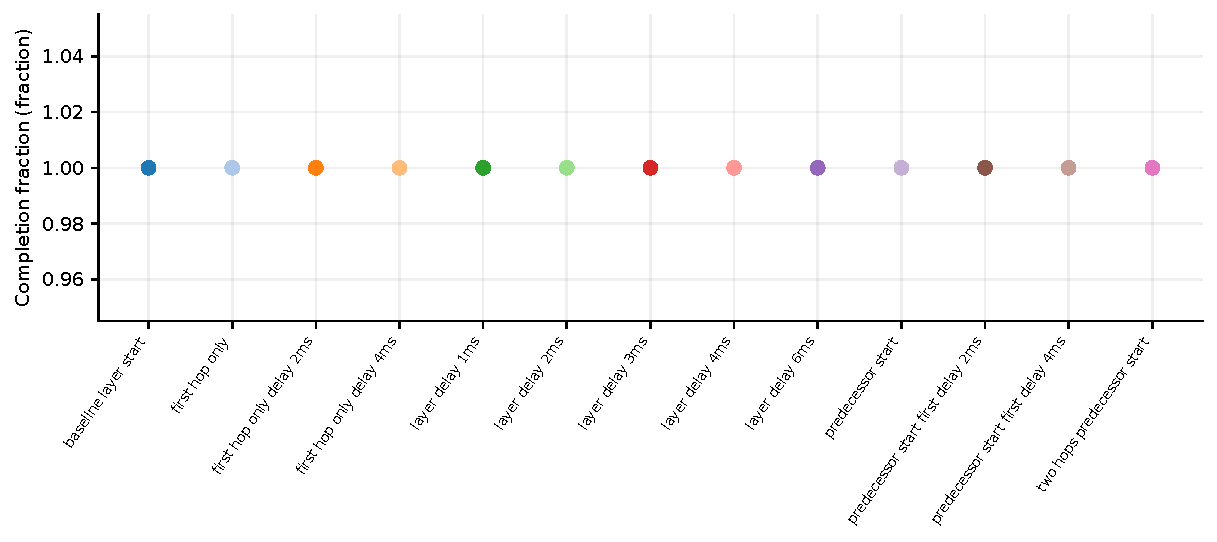
\includegraphics[width=.94\linewidth,height=.31\textheight,keepaspectratio]{figures/variants/torus_dijkstra_completion_rate.pdf}\captionof{figure}{Thirteen Dynamic launch variants, M=4 and C=3; zero-delay structural rules and delay sensitivities are distinguished in the definitions.}\end{center}
\begin{center}{\scriptsize\setlength{\tabcolsep}{3pt}
\begin{tabular}{lrr}
\toprule
Variant & Mean $\pm$ SD & n \\
\midrule
baseline-layer-start & $1.000\pm0.000$ & 6 \\
first-hop-only & $1.000\pm0.000$ & 6 \\
first-hop-only-delay-2ms & $1.000\pm0.000$ & 6 \\
first-hop-only-delay-4ms & $1.000\pm0.000$ & 6 \\
layer-delay-1ms & $1.000\pm0.000$ & 6 \\
layer-delay-2ms & $1.000\pm0.000$ & 6 \\
layer-delay-3ms & $1.000\pm0.000$ & 6 \\
layer-delay-4ms & $1.000\pm0.000$ & 6 \\
layer-delay-6ms & $1.000\pm0.000$ & 6 \\
predecessor-start & $1.000\pm0.000$ & 6 \\
predecessor-start-first-delay-2ms & $1.000\pm0.000$ & 6 \\
predecessor-start-first-delay-4ms & $1.000\pm0.000$ & 6 \\
two-hops-predecessor-start & $1.000\pm0.000$ & 6 \\
\bottomrule\end{tabular}}
\captionof{table}{All thirteen variants; n counts byte-distinct trace/physics runs, not conceptual aliases.}
{\footnotesize\href{https://github.com/sanjeevkrishnaa/Compiler-Driven-ACE/blob/codex/ace-scheduler-correctness/docs/latex/qft96_final/data/variants_torus_dijkstra_completion_rate.csv}{Exact CSV values and sample counts}}
\end{center}